% !TeX spellcheck = es_MX
\documentclass[12pt, a4paper, titlepage]{report}
\usepackage[spanish]{babel}
\usepackage[utf8]{inputenc}
\usepackage[linesnumbered,lined,boxed,commentsnumbered]{algorithm2e}
\usepackage{enumitem,kantlipsum}
\usepackage{array}
\usepackage{placeins}
% Códigos y codificación para caracteres en español
\usepackage{listings}
\usepackage{color}
\lstset{literate=
  {á}{{\'a}}1 {é}{{\'e}}1 {í}{{\'i}}1 {ó}{{\'o}}1 {ú}{{\'u}}1
  {Á}{{\'A}}1 {É}{{\'E}}1 {Í}{{\'I}}1 {Ó}{{\'O}}1 {Ú}{{\'U}}1
  {à}{{\`a}}1 {è}{{\`e}}1 {ì}{{\`i}}1 {ò}{{\`o}}1 {ù}{{\`u}}1
  {À}{{\`A}}1 {È}{{\'E}}1 {Ì}{{\`I}}1 {Ò}{{\`O}}1 {Ù}{{\`U}}1
  {ä}{{\"a}}1 {ë}{{\"e}}1 {ï}{{\"i}}1 {ö}{{\"o}}1 {ü}{{\"u}}1
  {Ä}{{\"A}}1 {Ë}{{\"E}}1 {Ï}{{\"I}}1 {Ö}{{\"O}}1 {Ü}{{\"U}}1
  {â}{{\^a}}1 {ê}{{\^e}}1 {î}{{\^i}}1 {ô}{{\^o}}1 {û}{{\^u}}1
  {Â}{{\^A}}1 {Ê}{{\^E}}1 {Î}{{\^I}}1 {Ô}{{\^O}}1 {Û}{{\^U}}1
  {œ}{{\oe}}1 {Œ}{{\OE}}1 {æ}{{\ae}}1 {Æ}{{\AE}}1 {ß}{{\ss}}1
  {ű}{{\H{u}}}1 {Ű}{{\H{U}}}1 {ő}{{\H{o}}}1 {Ő}{{\H{O}}}1
  {ç}{{\c c}}1 {Ç}{{\c C}}1 {ø}{{\o}}1 {å}{{\r a}}1 {Å}{{\r A}}1
  {€}{{\EUR}}1 {£}{{\pounds}}1
}
%%Appendix
\usepackage[toc,page]{appendix}

%%Tablas
\usepackage{tabularx}

%%otros
\usepackage{float}
\usepackage{subfig}
\usepackage{comment}

% http://ctan.org/pkg/booktabs
\usepackage{booktabs}
\newcommand{\tabitem}{~~\llap{\textbullet}~~}

%%Imágenes
\usepackage{graphicx}

%%Colores de texto 
\usepackage{xcolor}
\usepackage{colortbl}

%%Links
\usepackage[hidelinks]{hyperref}

%%Comentarios
\usepackage{verbatim}

%%PARA IMÁGENES EN LÍNEA
%\usepackage[english]{babel}

%%Acrónimos
\usepackage[acronym]{glossaries}

%%Glosario
\usepackage{glossaries}

\usepackage{pdfpages}

%%ESTILO DE CÓDIGO
\lstdefinestyle{codeStyle}{
	backgroundcolor=\color{backcolour}, commentstyle=\color{commentcolor},
	keywordstyle=\color{guindapoli},
	numberstyle=\tiny\color{azulescom},
	stringstyle=\color{azulfuerte},
	basicstyle=\ttfamily\footnotesize,
	breakatwhitespace=false, 
	breaklines=true, 
	captionpos=b,
	keepspaces=true,
	numbers=left,
	numbersep=5pt,
	showspaces=false,
	showstringspaces=false,
	showtabs=false,
	tabsize=3
}
\definecolor{delim}{RGB}{20,105,176}

%% JSON
\lstdefinelanguage{json}{
	basicstyle=\normalfont\ttfamily,
	numbers=left,
	numberstyle=\tiny\color{azulescom},
	stringstyle=\color{azulfuerte},
	stepnumber=1,
	numbersep=8pt,
	showstringspaces=false,
	breaklines=true,
	backgroundcolor=\color{backcolour},
	literate=
	*{0}{{{\color{azulfuerte}0}}}{1}
	{1}{{{\color{azulfuerte}1}}}{1}
	{2}{{{\color{azulfuerte}2}}}{1}
	{3}{{{\color{azulfuerte}3}}}{1}
	{4}{{{\color{azulfuerte}4}}}{1}
	{5}{{{\color{azulfuerte}5}}}{1}
	{6}{{{\color{azulfuerte}6}}}{1}
	{7}{{{\color{azulfuerte}7}}}{1}
	{8}{{{\color{azulfuerte}8}}}{1}
	{9}{{{\color{azulfuerte}9}}}{1}
	{:}{{{\color{guindapoli}{:}}}}{1}
	{,}{{{\color{guindapoli}{,}}}}{1}
	{\{}{{{\color{guindapoli}{\{}}}}{1}
	{\}}{{{\color{guindapoli}{\}}}}}{1}
	{[}{{{\color{guindapoli}{[}}}}{1}
	{]}{{{\color{guindapoli}{]}}}}{1},
}

\lstset{style=codeStyle}


\definecolor{lightgray}{rgb}{.9,.9,.9}
\definecolor{darkgray}{rgb}{.4,.4,.4}
\definecolor{purple}{rgb}{0.65, 0.12, 0.82}

%% Javascript
\lstdefinelanguage{JavaScript}{
	keywords={typeof, new, true, false, catch, function, return, null, catch, switch, var, if, in, while, do, else, case, break, let, continue},
	keywordstyle=\color{blue}\bfseries,
	ndkeywords={class, export, boolean, throw, implements, import, this},
	ndkeywordstyle=\color{darkgray}\bfseries,
	identifierstyle=\color{black},
	sensitive=false,
	comment=[l]{//},
	morecomment=[s]{/*}{*/},
	commentstyle=\color{purple}\ttfamily,
	stringstyle=\color{red}\ttfamily,
	morestring=[b]',
	morestring=[b]"
}

\lstset{
	language=JavaScript,
	backgroundcolor=\color{lightgray},
	extendedchars=true,
	basicstyle=\footnotesize\ttfamily,
	showstringspaces=false,
	showspaces=false,
	numbers=left,
	numberstyle=\footnotesize,
	numbersep=9pt,
	tabsize=2,
	breaklines=true,
	showtabs=false,
	captionpos=b
}
%% ESTO ES PYTHON

\definecolor{maroon}{cmyk}{0, 0.87, 0.68, 0.32}
\definecolor{halfgray}{gray}{0.55}
\definecolor{ipython_frame}{RGB}{207, 207, 207}
\definecolor{ipython_bg}{RGB}{247, 247, 247}
\definecolor{ipython_red}{RGB}{186, 33, 33}
\definecolor{ipython_green}{RGB}{0, 128, 0}
\definecolor{ipython_cyan}{RGB}{64, 128, 128}
\definecolor{ipython_purple}{RGB}{170, 34, 255}

\lstset{
	breaklines=true,
	extendedchars=true,
	literate=
	{á}{{\'a}}1 {é}{{\'e}}1 {í}{{\'i}}1 {ó}{{\'o}}1 {ú}{{\'u}}1
	{Á}{{\'A}}1 {É}{{\'E}}1 {Í}{{\'I}}1 {Ó}{{\'O}}1 {Ú}{{\'U}}1
	{à}{{\`a}}1 {è}{{\`e}}1 {ì}{{\`i}}1 {ò}{{\`o}}1 {ù}{{\`u}}1
	{À}{{\`A}}1 {È}{{\'E}}1 {Ì}{{\`I}}1 {Ò}{{\`O}}1 {Ù}{{\`U}}1
	{ä}{{\"a}}1 {ë}{{\"e}}1 {ï}{{\"i}}1 {ö}{{\"o}}1 {ü}{{\"u}}1
	{Ä}{{\"A}}1 {Ë}{{\"E}}1 {Ï}{{\"I}}1 {Ö}{{\"O}}1 {Ü}{{\"U}}1
	{â}{{\^a}}1 {ê}{{\^e}}1 {î}{{\^i}}1 {ô}{{\^o}}1 {û}{{\^u}}1
	{Â}{{\^A}}1 {Ê}{{\^E}}1 {Î}{{\^I}}1 {Ô}{{\^O}}1 {Û}{{\^U}}1
	{œ}{{\oe}}1 {Œ}{{\OE}}1 {æ}{{\ae}}1 {Æ}{{\AE}}1 {ß}{{\ss}}1
	{ç}{{\c c}}1 {Ç}{{\c C}}1 {ø}{{\o}}1 {å}{{\r a}}1 {Å}{{\r A}}1
	{€}{{\EUR}}1 {£}{{\pounds}}1
}

\lstdefinelanguage{python}{
	morekeywords={access,and,break,class,continue,def,del,elif,else,except,exec,finally,for,from,global,if,import,in,is,lambda,not,or,pass,print,raise,return,try,while},
	morekeywords=[2]{abs,all,any,basestring,bin,bool,bytearray,callable,chr,classmethod,cmp,compile,complex,delattr,dict,dir,divmod,enumerate,eval,execfile,file,filter,float,format,frozenset,getattr,globals,hasattr,hash,help,hex,id,input,int,isinstance,issubclass,iter,len,list,locals,long,map,max,memoryview,min,next,object,oct,open,ord,pow,property,range,raw_input,reduce,reload,repr,reversed,round,set,setattr,slice,sorted,staticmethod,str,sum,super,tuple,type,unichr,unicode,vars,xrange,zip,apply,buffer,coerce,intern},
	sensitive=true,
	morecomment=[l]\#,
	morestring=[b]',
	morestring=[b]",
	morestring=[s]{'''}{'''},
	morestring=[s]{"""}{"""},
	morestring=[s]{r'}{'},
	morestring=[s]{r"}{"},
	morestring=[s]{r'''}{'''},
	morestring=[s]{r"""}{"""},
	morestring=[s]{u'}{'},
	morestring=[s]{u"}{"},
	morestring=[s]{u'''}{'''},
	morestring=[s]{u"""}{"""},
	% {replace}{replacement}{lenght of replace}
	% *{-}{-}{1} will not replace in comments and so on
	literate=
	{á}{{\'a}}1 {é}{{\'e}}1 {í}{{\'i}}1 {ó}{{\'o}}1 {ú}{{\'u}}1
	{Á}{{\'A}}1 {É}{{\'E}}1 {Í}{{\'I}}1 {Ó}{{\'O}}1 {Ú}{{\'U}}1
	{à}{{\`a}}1 {è}{{\`e}}1 {ì}{{\`i}}1 {ò}{{\`o}}1 {ù}{{\`u}}1
	{À}{{\`A}}1 {È}{{\'E}}1 {Ì}{{\`I}}1 {Ò}{{\`O}}1 {Ù}{{\`U}}1
	{ä}{{\"a}}1 {ë}{{\"e}}1 {ï}{{\"i}}1 {ö}{{\"o}}1 {ü}{{\"u}}1
	{Ä}{{\"A}}1 {Ë}{{\"E}}1 {Ï}{{\"I}}1 {Ö}{{\"O}}1 {Ü}{{\"U}}1
	{â}{{\^a}}1 {ê}{{\^e}}1 {î}{{\^i}}1 {ô}{{\^o}}1 {û}{{\^u}}1
	{Â}{{\^A}}1 {Ê}{{\^E}}1 {Î}{{\^I}}1 {Ô}{{\^O}}1 {Û}{{\^U}}1
	{œ}{{\oe}}1 {Œ}{{\OE}}1 {æ}{{\ae}}1 {Æ}{{\AE}}1 {ß}{{\ss}}1
	{ç}{{\c c}}1 {Ç}{{\c C}}1 {ø}{{\o}}1 {å}{{\r a}}1 {Å}{{\r A}}1
	{€}{{\EUR}}1 {£}{{\pounds}}1
	%
	{^}{{{\color{ipython_purple}\^{}}}}1
	{=}{{{\color{ipython_purple}=}}}1
	%
	{+}{{{\color{ipython_purple}+}}}1
	{*}{{{\color{ipython_purple}$^\ast$}}}1
	{/}{{{\color{ipython_purple}/}}}1
	%
	{+=}{{{+=}}}1
	{-=}{{{-=}}}1
	{*=}{{{$^\ast$=}}}1
	{/=}{{{/=}}}1,
	literate=
	*{-}{{{\color{ipython_purple}-}}}1
	{?}{{{\color{ipython_purple}?}}}1,
	%
	identifierstyle=\color{black}\ttfamily,
	commentstyle=\color{ipython_cyan}\ttfamily,
	stringstyle=\color{ipython_red}\ttfamily,
	keepspaces=true,
	showspaces=false,
	showstringspaces=false,
	rulecolor=\color{ipython_frame},
	frame=single,
	frameround={t}{t}{t}{t},
	framexleftmargin=6mm,
	numbers=left,
	numberstyle=\tiny\color{halfgray},
	backgroundcolor=\color{ipython_bg},
	% extendedchars=true,
	basicstyle=\scriptsize,
	keywordstyle=\color{ipython_green}\ttfamily,
}
%------------------------------------------------ESTABLECER COLORES------------------------------------------------%

\definecolor{guindapoli}{RGB}{102, 0, 51}
\definecolor{azulescom}{RGB}{0, 0, 102}
\definecolor{azulclaro}{RGB}{222, 232, 255}
\definecolor{azulfuerte}{RGB}{60, 150, 250}

%------------------------------------------------COLORES PARA CÓDIGO------------------------------------------------%

\definecolor{commentcolor}{RGB}{ 192, 192, 192 }
\definecolor{backcolour}{RGB}{ 249, 249, 249 }

%------------------------------------------------FIN DE COLORES------------------------------------------------%

%------------------------------------------------GLOSARIO------------------------------------------------%

\makeglossaries
\newglossaryentry{Convolucional}
{
	name={Convolucional},
	text={convolucional},
	description={Es un operador matemático el cual transforma dos funciones en una tercera función.\cite{refRAE}}
}
\newglossaryentry{Recurrente}{
	name={Recurrente},
	text={recurrente},
	description={Algo que vuelve a ocurrir o a aparecer después de un intervalo.\cite{refRAE}}
}
\newglossaryentry{Reconocimiento}{
	name={Reconocimiento},
	text={reconocimiento},
	description={Examinar algo o a alguien para así poder conocer su identidad, estado, naturaleza y circunstancias. Distinguir o identificar a una persona o una cosa entre varas por una serie de características.\cite{refOxfordLex}}
}
\newglossaryentry{Aprende}{
	name={Aprende},
	text={aprende},
	description={Adquirir el conocimiento de algo por medio del estudio, análisis o de la experiencia.\cite{refRAE}}
}
\newglossaryentry{Sistema}{
	name={Sistema},
	text={sistema},
    description={Conjunto de elementos con relaciones de interacción e interdependencia las cuales le confieren entidad propia al formar un todo unificado.\cite{refSistema}}
}
\newglossaryentry{Estado}{
	name={Estado},
	text={estado},
    description={Situación en que se encuentra alguien o algo, y en especial cada uno de sus sucesivos modos de ser o estar.\cite{refRAE}}
}
\newglossaryentry{Armonia}{
	name={Armonía},
	text={armonía},
    description={Unión y combinación de sonidos simultáneos y diferentes, pero acordes.\cite{refRAE}}
}
\newglossaryentry{Melodia}{
	name={Melodía},
	text={melodía},
    description={Es una sucesión lineal ordenada y coherente de sonidos musicales los cuales forman una unidad estructurada con un sentido musical, independiente del acompañamiento. \\Sucesión de sonidos que por su manera de combinarse resulta agradable de oír.\cite{refOxfordLex}}
}
\newglossaryentry{Estrofa}{
	name={Estrofa},
	text={estrofa},
    description={Conjunto de versos que generalmente se ajustan a una medida y a un ritmo determinado y constante.\cite{refRAE}}
}
\newglossaryentry{Acordes}{
	name={Acordes},
	text={acordes},
    description={Conjunto de notas musicales sonando al mismo tiempo.\cite{refRAE}}
}
\newglossaryentry{Estocastico}{
	name={Estocástico},
	text={estocástico},
    description={Que está sometido al azar y que es un objeto de análisis estadístico.\cite{refRAE}}
}
\newglossaryentry{Maquinas de Estados Finitos}{
	name={Máquinas de Estados Finitos},
	text={máquinas de estados finitos},
    description={Conocidas también como Finite State Machines por su traducción en inglés, nos sirven para realizar procesos bien definidos en un tiempo discreto. Reciben una entrada, realizan un proceso y nos entregan una salida.\cite{refMaquinasFinitas}}
}

%------------------------------------------------FINAL DE GLOSARIO------------------------------------------------%


%------------------------------------------------ACRÓNIMOS------------------------------------------------%

\newacronym{mvc}{MVC}{Modelo-Vista-Controlador}
\newacronym{orm}{ORM}{Object Relational Manager}
\newacronym{wsgi}{WSGI}{Web Server Gateway Interface}
\newacronym{dbms}{DBMS}{Sistema de gestión de base de datos}
\newacronym{bert}{BERT}{Bidirectional Encoder Representations from Transformers}
\newacronym{pln}{PLN}{Procesamiento del Lenguaje Natural}
\newacronym{mlm}{MLM}{Modelado de Lenguaje Enmascarado}
\newacronym{gpt}{GPT}{Generative Pretrained Transformer}
\newacronym{bpe}{BPE}{Byte Pair Encoding}
\newacronym{wip}{WIP}{Work In Progress}
\newacronym{cls}{CLS}{Classification}
\newacronym{sep}{SEP}{Separate}
\newacronym{json}{JSON}{Javascript Object Notation}
\newacronym{url}{URL}{Uniform Source Locator}
\newacronym{http}{HTTP}{Hypertext Transfer Protocol}
\newacronym{tcp}{TCP}{Transmission Control Protocol}
\newacronym{udp}{UDP}{User Datagram Protocol}
\newacronym{imap}{IMAP}{Internet Message Access Protocol}
\newacronym{pop}{POP}{Post Office Protocol}
\newacronym{smtp}{SMTP}{Simple Mail Transfer Protocol}
\newacronym{vps}{VPS}{Virtual Private Server}
\newacronym{ssl}{SSL}{Secure Socket Layer}
\newacronym{fqdn}{FQDN}{Fully Qualified Domain Name}
\newacronym{aws}{AWS}{Amazon Web Services}
\newacronym{gpu}{GPU}{Graphic Processor Unit}
\newacronym{ec2}{EC2}{Elastic Compute Cloud}
\newacronym{ui}{UI}{User Interface}
\newacronym{api}{API}{Application Programm Interface}
\newacronym{gcp}{GCP}{Google Cloud Platform}
\newacronym{sdk}{SDK}{Software Development Kit}
\newacronym{html}{HTML}{Hypertext Markup Language}
\newacronym{css}{CSS}{Cascading Style Sheet}
\newacronym{ecma}{ECMA}{European Computer Manufacturers Association}
\newacronym{https}{HTTPS}{Hypertext Transfer Protocol Secure}
\newacronym{tls}{TLS}{Transport Layer Security}
\newacronym{sql}{SQL}{Structured Query Language}
\newacronym{cad}{CAD}{Computer Aided Design}
\newacronym{cli}{CLI}{Command Line Interface}
\newacronym{s3}{S3}{Simple Storage Service}
\newacronym{hdd}{HDD}{Hard Drive Disk}
\newacronym{ssd}{SSD}{Solid State Drive}
\newacronym{iso}{ISO}{International Standardization Organization}
\newacronym{xml}{XML}{Extensible Markup Language}
\newacronym{svg}{SVG}{Scalable Vector Graphics}
\newacronym{rnn}{RNN}{Recurrent Neural Network}
\newacronym{lstm}{LSTM}{Long Short Term Memory}
%------------------------------------------------FINAL DE ACRÓNIMOS------------------------------------------------%

\begin{document}
	%%PARA QUE DETECTE HASTA SUBSUBSECTION
	\setcounter{secnumdepth}{3}
	
%%%%%%%%%%%%%%%%%%%%%%%%%%%%%%%%%%%%%%%%%%%%%%%%%%%%%%%%%
%                                                       																																		  %
%                                                      																																	  		  %
%              																	PORTADA  																				  			 %
%                                                      																																			  %
%                                                      																																			  %
%%%%%%%%%%%%%%%%%%%%%%%%%%%%%%%%%%%%%%%%%%%%%%%%%%%%%%%%%
	\begin{titlepage}	
		
		\newcommand{\HRule}{\rule{\linewidth}{0.5mm}}									%%%\left
 																					%%%
\begin{minipage}{0.48\textwidth} \begin{flushleft}

\includegraphics[scale = 0.10]{imagenes/MarcoTeorico/logoescom.png}
\end{flushleft}\end{minipage}
\begin{minipage}{0.48\textwidth} \begin{flushright}

\includegraphics[scale = 0.55]{imagenes/MarcoTeorico/logoipn.png}
\end{flushright}\end{minipage}

													 								%%%
\vspace*{.25cm}								%%%
		
		\begin{center}
			
			\begin{LARGE}
				\textcolor{guindapoli}{INSTITUTO POLITÉCNICO NACIONAL}\\
			\end{LARGE}	
			
			\vspace*{0.2in}
			
			\begin{Large}
				\textcolor{azulescom}{ESCUELA SUPERIOR DE CÓMPUTO}\\
			\end{Large}		
			
			\vspace*{0.4in}
			
			\begin{large}
				Trabajo Terminal\\
			\end{large}
			
			\vspace*{0.2in}
			
			\begin{Large}
				\textbf{Generador de versos musicales en el idioma
inglés por medio de procesamiento de lenguaje
natural y redes neuronales}\\
			\end{Large}
			
			\vspace*{0.2in}
			
			\begin{large}
				TT2020-B002\\
			\end{large}
			
			\vspace*{0.2in}
			
			\rule{80mm}{.1mm}\\
			\vspace*{0.1in}
			
			\begin{large}
				\begin{center}
					\textbf{Presentan}:\\
					Espinosa de los Monteros Lechuga Jaime Daniel\\
					Nava Romo Edgar Adrián\\
					Salgado Gómez Alfredo Emilio\\
				\end{center}
			\end{large}
			
			\begin{large}
				\textbf{Directores}:\\
				Olga Kolesnikova\\
				Ariel López Rojas\\
			\end{large}
			
		\end{center}
	
	\end{titlepage}

%%%%%%%%%%%%%%%%%%%%%%%%%%%%%%%%%%%%%%%%%%%%%%%%%%%%%%%%%
%                                                       																																		  %
%                                                      																																	  		  %
%              																	 ÍNDICE  																				  			 	  %
%                                                      																																			  %
%                                                      																																			  %
%%%%%%%%%%%%%%%%%%%%%%%%%%%%%%%%%%%%%%%%%%%%%%%%%%%%%%%%%
% Firma directores
\newpage
\section*{Firmas de Directores}

\vfill  % push the rest to the bottom of the page
\noindent 
\parbox[b]{0.4\linewidth}{% size of the first signature box
	\strut 
	Firmado por: \\[3cm]% This 2cm is the space for the signature under the names
	\hrule
	Profesor: Ariel López Rojas} 
\hspace{1cm} % distance between the two signature blocks 
\parbox[b]{0.4\linewidth}{% ...and the second one
	\strut 
	\\[3cm]% This 2cm is the space for the signature under the names
	\hrule
	Doctora Olga Kolesnikova} 
\par\vspace{1cm} 
\newpage
% Rename Appendice to Anexos
\renewcommand\appendixpagename{Índice}
\renewcommand\appendixtocname{Índice}
\appendixpageoff
	\begin{appendices}
		\renewcommand*\contentsname{{\textcolor{azulescom}{Índice.}}}
		\tableofcontents
		\newpage
		%%índice de figuras
		\renewcommand*\listfigurename{{\textcolor{azulescom}{Índice de figuras.}}}
		\listoffigures
		\newpage
		%%Índice de tablas
		\newpage
		\renewcommand*\listtablename{{\textcolor{azulescom}{Índice de cuadros.}}}
		\listoftables
	\end{appendices}
	
   \textcolor{guindapoli}{\part{Trabajo Terminal I}}
    
    \renewcommand\thechapter{\arabic{chapter}}
    \renewcommand{\appendixname}{Capítulo}
    \renewcommand{\lstlistingname}{C\'odigo}
    \renewcommand{\thepart}{}
    \renewcommand{\partname}{}
    %   %   %   %   %   %   %   %   %   %
    %		           Capítulo 1  				   %
    %   			Introducción 			    %
    %                               				  		 %
    %   %   %   %   %   %   %   %   %	 %
    \chapter{\textcolor{azulescom}{Introducción}}
    La industria musical obtiene ganancias a través de la creación y divulgación de la música física y digitalmente (Bourreau and Gensollen 2006 \cite{Bourreau_and_Gensollen}), dejando que aficionados y emprendedores de la música no tengan oportunidad de avanzar en su carrera por falta de creatividad, tiempo y/o recursos, haciendo que la creación de nuevas letras para sus canciones sea un gran obstáculo, nuestra propuesta implica la utilización de nuevas tecnologías que permitan la generación de letras para integrar con sus canciones. Esta es una de las tareas más populares y desafiantes en el área de procesamiento del lenguaje natural. Hay una gran cantidad de trabajos (Generating Text with Recurrent Neural Networks \cite{Generating_Text_with_RNN}, Convolutional Neural Networks for Sentence Classification\cite{CNN_for_Sentence_Classification}) que proponen generar texto utilizando redes neuronales recurrentes y/o convolucionales. Sin embargo, la mayoría de los trabajos actuales solo se enfocan en generar una o varias oraciones, ni siquiera un párrafo largo y mucho menos una canción completa.\\\\
    Las letras de canciones, como un tipo de texto, tienen algunas características propias, estas se constituyen de rimas, versos, coros y en algunos casos, patrones de repetición. Coro se refiere a la parte de una canción que se repite sin modificaciones dentro de la misma después de un verso, mientras que en el verso suelen cambiar una o varias líneas que lo componen. Estas características particulares hacen que generar letras musicales sea mucho más difícil que textos normales.\\\\
    La mayoría de las investigaciones actuales sobre generación de letras vienen con muchas condiciones, como dar una pieza de melodía (Automatic Generation of Melodic Accompaniments for Lyrics \cite{Automatic_Generation_of_Melodic_Accompaniments_for_Lyrics}), o solo generar un tipo específico de letra (Conditional Rap Lyrics Generation with Denoising Autoencoders \cite{Conditional_Rap_Lyrics_Generation}). Sin embargo, la generación de letras por medio de inteligencia artificial dado un estilo y tema en particular, ha sido muy poco trabajado y debido a esto planeamos centrarnos en este nuevo problema. Estamos interesados en ver si el modelo propuesto puede aprender diferentes características de un género musical y generar letras que sean acorde a este. Actualmente, en el mercado se encuentran cuatro aplicaciones web que tienen una funcionalidad similar a la propuesta en este Trabajo Terminal:\par
    
    \begin{itemize}
    	\item These lyrics do not exist.
    	\item Bored humans - lyrics\_generator.
    	\item DeepBeat.
    	\item Premium Lyrics.
    \end{itemize}
	\newpage
	En el cuadro 1 que se presenta a continuación, se muestran las características de aplicaciones web similares y comparándolas con nuestra propuesta:
	\begin{table}[!htbp]
		\caption[Productos similares]{Resumen de productos similares comparados con nuestra propuesta}
		\begin{tabular}{|m{3.5cm}|m{6.5cm}|m{3.5cm}|}
			\hline    			
			\rowcolor{guindapoli}
			\hfil {\textbf{\textcolor{white}{Software}}} & \hfil {\textbf{\textcolor{white}{Características}}} & \hfil {\textbf{\textcolor{white}{Precio}}} \\
			\hline
			These Lyrics do not Exist & Aplicación web que genera letras completamente originales de varios temas, hace uso de IA para generar coros y versos originales; se puede escoger el tema principal de la letra, género musical e incluso el estado de ánimo al que iría dirigido. & Gratuito (Contiene Anuncios) \\
			\hline
			Boredhumans lyrics\_generator & Aplicación web en el que la IA fue entrenada con una base de datos con miles de textos para generar canciones totalmente nuevas. La letra que crea es única y no una copia de alguna que exista actualmente, sin embargo, no permite modificar la letra. & \hfil Gratuito \\
			\hline
			\hfil DeepBeat & Aplicación web que por medio de IA genera letras de música enfocada principalmente en el género rap. Si una línea no es del agrado se puede sustituir por alguna de las otras propuestas de las que ofrece. & \hfil Gratuito \\
			\hline
			\hfil Premium Lyrics & Aplicación web que proporciona versos compuestos en distintos idiomas por artistas independientes que se escogen manualmente de acuerdo a su originalidad y calidad. & \$3 a \$75 Dólares por letra musical \\
			\hline
			\hfil Nuestra propuesta & Aplicación web que haciendo uso de una IA va a generar letras musicales originales a partir de un género musical en exclusivo, lo que asegurará un resultado original con coros y versos distintos cada vez que se utilice. & \hfil Gratuito \\
			\hline
		\end{tabular}\label{table:Propuestas}% is used to refer this table in the text
\end{table}
\newpage
	\section{Objetivos}
	\subsection{Objetivo general}
	Crear una herramienta de apoyo para estudiantes o aficionados interesados en este rubro que se les dificulte componer nuevas letras musicales de un solo género musical debido a la carencia de creatividad, la falta de conocimientos en la estructura del género o que no tengan inspiración suficiente para poder crear nuevas canciones, esto con el fin de impulsar la carrera de futuros artistas en la industria musical que no tengan los suficientes recursos para poder contratar servicios particulares de compositores.
	
	\subsection{Objetivos particulares}
		\begin{itemize}
			\item Generar un conjunto de datos (dataset) con letras musicales en un género musical para efecto de entrenamiento en la red semántica.
    		\item Hacer uso de alguna herramienta que utilice aprendizaje automático (machine learning) e implementar su uso en la nube para ayudar a procesar las letras musicales en un género específico.
    		\item Implementar un módulo analizador de semántica para entrenar redes neuronales.
    		\item Desarrollar una interfaz web intuitiva en versión prototipo que utilice una aplicación web alojada en la nube para tener una visualización del verso musical generado a partir de un género.
    	\end{itemize}
		
    	\section{Justificación}
    	El crear nuevas composiciones musicales puede llegar a ser muy difícil, estresante e incluso agotador para cualquier aficionado o incluso algunos expertos en este medio, esto se debe a la falta de creatividad y/o tiempo de quien lo quiera realizar \cite{What_about_the_music}. En ocasiones se pueden contratar servicios particulares para la producción de letras musicales, sin embargo, puede ser muy costoso y en ocasiones el resultado final no alcanza a llenar las expectativas de la inversión que se hace; por ende, se pretende crear una herramienta para estudiantes, aficionados o cualquier persona interesada en este rubro que se les dificulte componer nuevas letras musicales.\\\\
    	Normalmente estas son creadas por el humano y tienden a estar compuestas por patrones de acuerdo al género musical \cite{genero_musical_en_la_musica_popular}. Algunos ejemplos de estos patrones pueden ser las rimas, enunciados, frases cortas y que tengan una semántica correcta, estos pueden ser encontrados utilizando algoritmos de inteligencia artificial, específicamente, procesamiento de lenguaje natural y una investigación profunda en la composición de letras en estos géneros.\\\\
    	Se eligió el idioma inglés debido a que existe una gran cantidad de datasets para procesar, al igual que herramientas y documentación para este idioma.\\\\
    	Nos proponemos orientar esta solución en un entorno utilizando la nube, donde la información de configuración, servicios y datos necesarios pueden mantenerse de forma independiente a la implementación, facilitando la adaptación y flexibilidad de la plataforma.\\\\
    	Nuestro proyecto ayudará al usuario utilizando herramientas como el procesamiento de lenguaje natural, redes neuronales, aprendizaje de máquina (machine learning) y servidores en la nube. Se hará uso de un conjunto de datos (dataset) y herramientas alojadas en la nube (Google Cloud Platform o Amazon Web Services) para procesar estos datos; se pretende utilizar un módulo que encuentre patrones por medio de redes neuronales para analizar la semántica mediante técnicas y herramientas ya existentes de procesamiento de lenguaje natural. Se van a realizar pruebas y experimentos con estas herramientas antes de la implementación (BERT \cite{Bert}, spaCy\cite{spaCy}) para poder generar versos. A su vez se va a desarrollar una interfaz web intuitiva en versión prototipo donde el usuario va a poder utilizar esta herramienta la cual le va a mostrar la letra musical que se va a generar en ese momento.\\\\
    	A diferencia de los proyectos señalados en la Tabla \ref{table:Propuestas} nuestra propuesta se va a centrar en generar letras musicales con métodos y tecnologías distintas a los que se usaron, esto es, aunque se utilicen los mismos géneros musicales se tendrán resultados completamente diferentes con propuestas distintas.\\\\
    	En el desarrollo de este proyecto haremos uso de los conocimientos adquiridos durante el transcurso de la carrera. Se van a utilizar técnicas de diseño de proyectos aprendidas en el curso de Ingeniería de Software, se van a aplicar los conocimientos de programación adquiridos en unidades de aprendizaje como Inteligencia Artificial, Procesamiento de Lenguaje Natural, Web Application Development, Programación Orientada a Objetos, Análisis de Algoritmos, así como técnicas de construcción de documentos y análisis de semántica vistas en Análisis y Diseño orientado a Objetos y Comunicación Oral y Escrita.
    	
	    \section{Metodología}
	    Para el desarrollo de este trabajo terminal se utilizará la metodología ágil Scrumban, que combina algunas partes de la metodología Scrum y Kanban, debido a que este proceso de gestión reduce la complejidad al momento de desarrollar un producto el cual tratará de satisfacer las necesidades de los clientes. Además, permite trabajar colaborando entre pares de manera eficiente, es decir, en equipo, para obtener el mejor resultado posible.\\\\
	    Scrumban combina la estructura utilizada por Scrum, con los métodos basados en el flujo y visualización de Kanban. Es decir, que permite a los equipos trabajar de manera ágil usando la metodología Scrum y la simplicidad de Kanban sin tener que utilizar las actualizaciones de roles y es más sencillo de adoptar.\\\\
	    En la siguiente tabla se pueden observar las principales diferencias entre las tres metodologías:
    
	    \begin{table}[htbp!]
	    	\caption[Comparación de metodologías ágiles]{Tabla comparativa de las distintos metodologías ágiles contempladas}
	    	\begin{tabular}{|m{1.75cm}|m{2.75cm}|m{2.75cm}|m{4.75cm}|}
	    		\hline    			
	    		\rowcolor{guindapoli}
	    		 & \hfil {\textbf{\textcolor{white}{Scrum}}} & \hfil {\textbf{\textcolor{white}{Kanban}}} & \hfil {\textbf{\textcolor{white}{Scrumban}}}\\
	    		\hline
	    		 \hfil Procesos & Iterativo e incremental desarrollando sprints & \hfil Continuo & Iterativo e incremental de forma continua desarrollando iteraciones \\
	    		 \hline
	    		 \hfil Personas & Las personas son el centro & Las personas son el pilar & Equipo motivado con personas como pilar y en el centro \\
	    		 \hline
	    		 \hfil Producto & Foco en la efectividad & Foco en la eficiencia & Balance entre efectividad y eficiencia \\
	    		 \hline
	    		 \hfil Organización & Mejora continua del producto & Mejora continua del proceso & Mejora continua del producto y del proceso\\
	    		 \hline
	    		 \hfil Equipo & De 3 a 9 personas & No hay limitaciones & El equipo no requiere de un número específico de integrantes \\
	    		 \hline
	    		 \hfil Roles & Scrum master, Product owner, Scrum team & Pueden incluir especialistas o integrantes generalizados & No requiere un rol específico \\
	    		 \hline
	    	\end{tabular}
	    \end{table}
	    Scrumban hace uso de iteraciones, las cuales monitorea con el apoyo de un recurso visual, como lo puede ser un tablero. Las reuniones para planificar se llevan a cabo cuando son necesarias para determinar las tareas a implementar hasta la próxima iteración. Para que estas iteraciones se mantengan cortas, se utiliza un límite de trabajo en progreso (\acrshort{wip} por sus siglas en inglés Work in Progress). Cuando \acrshort{wip} desciende de cierto nivel, se establece una acción para que el equipo sepa cuándo y qué tarea planificar a continuación.\\\\
	    \textbf{Iteración}\\
	    En Scrumban, las iteraciones son cortas para garantizar que el equipo pueda adaptarse al entorno cambiante durante el proyecto. La duración de estas iteraciones en este proyecto se medirán como máximo en lapsos de dos semanas.\\
	    \\
	     \textbf{Priorización}\\
	    Esta se da de tal forma que las tareas más importantes se colocan en la parte superior en la tabla de planificación seguidas por las tareas menos importantes.\\
	    Antes de llegar al tablero las tareas deben pasar por 3 etapas donde se van depurando las que se van a realizar para largo plazo (1 año), medio plazo (6 meses) y corto plazo (3 meses) siendo esta última de donde salen las tareas más claras que se pueden completar y que ganan mayor prioridad para la próxima iteración.\\
	    \\
	     \textbf{Principio de Elección}\\
	    Cada miembro del equipo elige una o varias tarea de la sección “Tareas Pendientes” que va a completar antes de la siguiente reunión.\\
	    \\
	     \textbf{Congelación de Funciones}\\
	    Se utiliza cuando hay una fecha límite del proyecto próxima, significando que sólo pueden trabajar sobre las tareas previamente pensadas sin cabida para implementar nuevas características.\\
	    \\
	     \textbf{Triaje}\\
	    Ocurre después de la congelación de funciones, es aquí donde el líder del proyecto decide las características en desarrollo que se completarán y cuáles quedarán sin terminar.\\
	    
	    \begin{figure}[H] 
	    	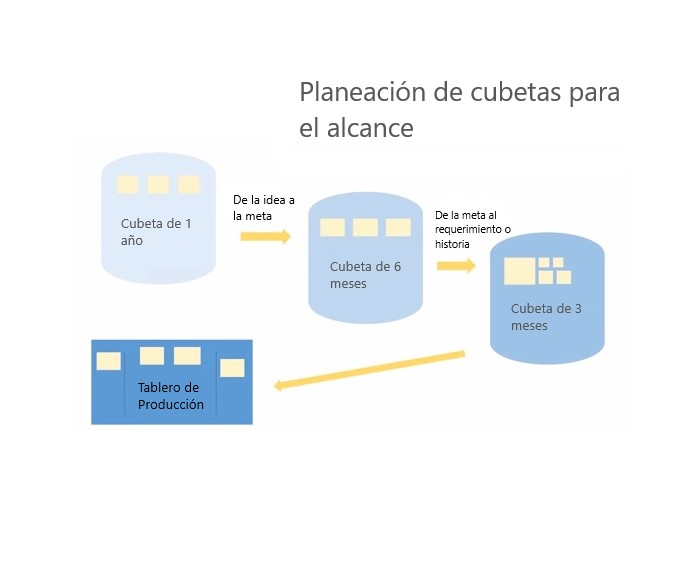
\includegraphics[width=12cm]{./imagenes/Introduccion/scrumban_buckets.jpg}
	    	\centering \caption{Funcionamiento de la planificación por cubetas}
	    \end{figure}
    
    	\subsection{Implementación}
    	En el proyecto se aplicará esta metodología utilizando la aplicación de Trello para llevar a cabo el tablero, contando con cuatro listas importantes:
    	\begin{itemize}
    		\item Scrum Backlog: Contará con las características generales de la iteración en la que se pretende trabajar.
    		\item To Do: Lista en la que cada integrante del equipo agrega funcionalidades tanto las que son funcionales como las que no lo son que tendrá el proyecto, en sus debidas reuniones se discutirá sobre la priorización de las tarjetas que se agreguen y cada integrante elegirá las que quiera desarrollar y cuántas pueda hacer.
    		\item In Progress: Cuando el integrante del equipo ya esta trabajando en alguna de las tareas que eligió, pasa a formar parte de esta lista, esto quiere decir que en la siguiente reunión que se tenga tendrá que dar sus debidos resultados o en su defecto, comentar que ya se terminó.
    		\item Done: Las tareas que forman parte de la iteración que ya se terminaron, van pasando a esta lista, dejando a las otras listas con menos tarjetas a realizar cada vez. Cuando ya estén todas las tareas realizadas, se puede volver a Backlog para poder proseguir con la siguiente iteración del proyecto, en caso de que queden tarjetas y las fechas límites estén próximas a terminar, se tendrán que parar las tareas que no sean vitales al proyecto para que se puedan realizar las tareas con más importancia.
    	\end{itemize} 
    	\subsection{Iteraciones}
    	El proyecto se dividirá en cuatro iteraciones por trabajo terminal, cada iteración tiene una duración establecida de cuatro semanas o un mes, dejando cada iteración de la siguiente manera:
    	\subsubsection*{Trabajo Terminal I}
    	\begin{itemize}
    		\item Se construirá una base de datos acorde al proyecto, la cual contendrá las letras musicales de distintos artistas, así como su género.
    		\item Se realizará una limpieza a los datos extraídos del dataset.
    		\item Se seleccionarán e implementarán las herramientas necesarias para trabajar en la construcción de un modelo utilizando redes neuronales.
    		\item Se generará un modelo en la nube para su entrenamiento utilizando las redes neuronales previamente elegidas.
    	\end{itemize}
    	\subsubsection*{Trabajo Terminal II}
    	\begin{itemize}
    		\item Se implementará la interfaz que el usuario final verá.
    		\item Se integrará el la interfaz con la aplicación que utiliza el modelo utilizando un servidor web.
    		\item Se realizarán las pruebas pertinentes, así como la re-ingeniería requerida.
    		\item Se desarrollará el manual técnico y el de usuario.
    	\end{itemize}
    
	    \newpage
        \section{Organización del documento}
            Para dar inicio a este trabajo terminal, presentamos de manera breve la estructura de este reporte, con el objetivo de que el lector pueda tener un mejor entendimiento del trabajo.

            \subsection*{Capítulo 2. Marco teórico}
                En esta parte del documento, se describen puntos esenciales de nuestro trabajo como definiciones, técnicas, herramientas, servicios, así como investigación realizada para llevar a cabo en la implementación dentro del trabajo. 
             
            \subsection*{Capítulo 3. Análisis}
                Dentro de este capitulo se hará un análisis tanto del problema propuesto, como sus posibles soluciones, se harán análisis de estudio en cuanto a la factibilidad técnica, operativa y económica con la finalidad de conocer los recursos necesarios para la elaboración de este trabajo terminal. Se mencionan las herramientas a utilizar y se explica de manera general la arquitectura del sistema y las historias de usuario del mismo.
             
            \subsection*{Capítulo 4. Diseño}
                En el cuarto capítulo, nos adentraremos en el desarrollo de las iteraciones propuestas, es decir, se encuentran los diagramas pertinentes para poder modelar nuestro trabajo terminal y proceder a la etapa de implementación. En este capítulo se desarrolla el diseño de cada parte del sistema y se muestra la interfaz de usuario propuesta junto con los requisitos de diseño.
             \begin{comment}
				%% PARA TT2
            \subsection{Capítulo 5. Desarrollo}
                En este capítulo mostraremos lo que se ha desarrollado para este Trabajo Terminal I (Iteración I, Iteración II, Iteración III, Iteración IV). Se muestra que se cumplan los requerimientos que se impusieron en la sección de análisis.
            
            \subsection{Capítulo 6. Avances y trabajo por hacer}
                En el último capítulo de este reporte, hablaremos de los avances que hemos logrado a lo largo de la asignatura de Trabajo Terminal I y además, exponemos el trabajo esperado para la asignatura de Trabajo Terminal II.
              \end{comment}   
%%%%%%%%%%%%%%%%%%%%%%%%%%%%%%%%%%%%%%%%%%%%%%%%%%%%%%%%%
%                                                       																																		  %
%                                                      																																	  		  %
%              																	 Capítulo 2  																				  			%
%                                                      						   Marco Teórico																					   %
%                                                      																																			  %
%%%%%%%%%%%%%%%%%%%%%%%%%%%%%%%%%%%%%%%%%%%%%%%%%%%%%%%%%        
 \chapter{\textcolor{azulescom}{Marco teórico}}
		\section{Inteligencia artificial}
		Por Inteligencia Artificial se entiende a una simulación de procesos computacionales cognitivos para que simulen el comportamiento de una mente humana, estos comportamientos abarcan diferentes áreas de investigación, como el razonamiento, aprendizaje, percepción, comunicación y la capacidad de desarrollarse en entornos más complejos.
		“La inteligencia no es una dimensión única, sino un espacio profusamente estructurado de capacidades diversas para procesar la información. Del mismo modo, la Inteligencia Artificial utiliza muchas técnicas diferentes para resolver una gran variedad de tareas que se encuentran en todas partes.” \cite{Inteligencia_Artificial}\\\\
		En ciencias de la computación, el término de inteligencia artificial hace referencia a cualquier inteligencia semejante a la humana presentado por una computadora o un equipo electrónico. De manera popular, la inteligencia artificial hace referencia a la capacidad de una computadora o máquina de imitar las facultades del cerebro humano, es decir, que es capaz de aprender mediante ejemplos y experiencias, así como reconocer objetos y clasificarlos, tomar decisiones, resolver problemas, entender y responder al lenguaje, igualmente combinar estas y otras capacidades para realizar funciones similares que un ser humano podría realizar. \cite{refInteligencia_Artificial2}\\\\
		Como objetivo, la Inteligencia Artificial pretende hacer un uso de los recursos tecnológicos para desarrollar modelos computacionales y poder resolver problemas del mundo real evolucionando constantemente.
	    \section{Redes neuronales}
	    Una red neuronal es una herramienta derivada de la inteligencia artificial que utiliza modelos matemáticos para ser utilizada como un mecanismo de predicción del texto.\\\\
		Las redes neuronales son una forma de hacer que las computadoras aprendan, donde la computadora aprende a realizar alguna tarea analizando ejemplos de entrenamiento. Por lo general, estos ejemplos han sido etiquetados previamente.\\\\
		Modelado vagamente en el cerebro humano, una red neuronal consiste en miles de millones de nodos que realizan procesamiento los cuales están densamente interconectados. En la actualidad las redes neuronales están organizadas como capas de nodos, y estas capas están “alimentadas hacia adelante” (feed-forward), es decir, la información que se mueve a través de ellas solo fluye en una sola dirección. Un solo nodo puede estar conectado a muchos nodos en capas inferiores de las cuales recibe información y a su vez, puede estar conectado a nodos en capas superiores a los cuales envía información.\\\\
		Cuando una red neuronal está siendo entrenada la información de entrenamiento pasa a alimentar las capas inferiores (de entrada), donde será procesada y pasada a capas posteriores donde será transformada hasta llegar a las capas superiores (de salida).\cite{refQueSonRedesNeu}

				\subsection{Neuronas}
						\subsubsection*{Neurona natural}
						La neurona es una de muchas células la cual representa a la unidad estructural y funcional del sistema nervioso. Esta trabaja transmitiendo la información a través de impulsos nerviosos o químicos, desde un lugar del cuerpo hacia otra parte de este.\\\\
						Dicho impulso nervioso o eléctrico viaja siempre en un mismo sentido, es decir, llega a la neurona mediante las dendritas, se procesa en el soma y posteriormente se transmite al axón, las neuronas no están en contacto entre sí, existe un espacio de separación denominado sinapsis o espacio sináptico. Una vez que el impulso nervioso llega al extremo final del axón este libera neurotransmisores al espacio sináptico transformando esta señal eléctrica en una señal química que en su funcionamiento, se introduce en la dendrita ubicada en la neurona contigua, desencadenando un impulso eléctrico en la receptora, repitiendo este proceso n veces hasta llegar a su destino final.\cite{refNeuronaNat}
						\begin{figure}[H]
							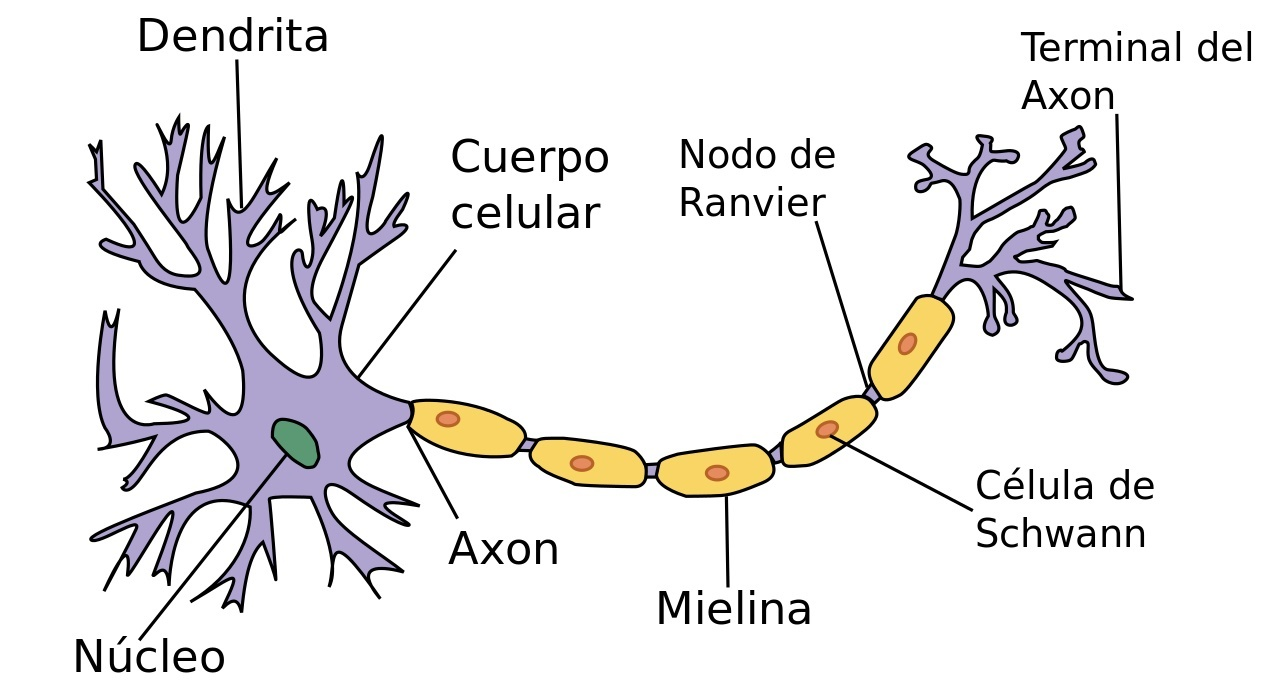
\includegraphics[width=12cm]{./imagenes/MarcoTeorico/Neurona.jpg}
							\centering  
							\caption{Estructura de una neurona \cite{refNeuronaNat2}}
						\end{figure}			
						\subsubsection*{Neurona artificial}
						La complejidad de las neuronas reales se abstrae mucho cuando se realiza el modelado de neuronas artificiales. Estas consisten básicamente en entradas, que se multiplican por pesos (fuerza de las respectivas señales), y luego calculada por una función matemática que determina la activación de la neurona. Otra función (que puede ser la de identidad) calcula la salida de la neurona artificial (a veces en dependencia de un cierto umbral). Las redes neuronales combinan neuronas artificiales para procesar información.\cite{refNeuronaArt}
						\begin{figure}[H] 
							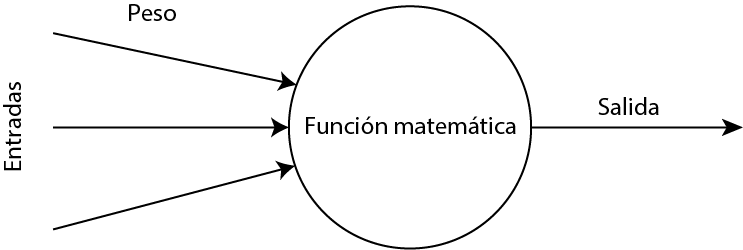
\includegraphics[width=12cm]{./imagenes/MarcoTeorico/NeuronaArt.png}
							\centering 
							\caption{Neurona artificial}
						\end{figure}
				\subsection{Aprendizaje de las redes neuronales}
				Si observamos la naturaleza, podremos ver que a pesar de existir muchos tipos de sistemas, los que  pueden aprender son altamente adaptables. En su búsqueda por adquirir conocimientos, estos sistemas utilizan información del mundo exterior y modifican la información que ya han recopilado o modifican su estructura interna. Eso es exactamente lo que hacen las redes neuronales. Adaptan y modifican su arquitectura logrando aprender. Para ser más precisos, las redes neuronales cambian los pesos de las conexiones según la entrada y salida deseada.\\\\
				¿Por qué tienen un peso?, bueno, si observamos la estructura de las redes neuronales, hay algunos componentes que podríamos cambiar, si queremos modificar su arquitectura. Por ejemplo, podríamos crear nuevas conexiones entre neuronas, eliminarlas y/o agregar más de estas. Incluso se podría modificar la función de entrada o la de activación. Resulta que cambiar los pesos es el enfoque más práctico. Además, la mayoría de los otros casos podrían cubrirse cambiando los pesos. La eliminación de una conexión, por ejemplo, se puede hacer estableciendo el peso en 0. Y una neurona se puede eliminar si establecemos los pesos de todas sus conexiones en cero.\cite{refAprendizajeRedes}\\\\
				El entrenamiento es un proceso necesario para toda red neuronal, y consiste en que la red se familiariza con el problema que necesita resolver. En la práctica, generalmente se tienen algunos datos recopilados en función de los cuales necesitamos crear nuestras predicciones, clasificación, o cualquier otro procesamiento. Estos datos se denominan conjunto de entrenamiento y según el comportamiento y la naturaleza, tenemos algunos tipos de aprendizajes:\\
				\begin{itemize}
					\item \textbf{Aprendizaje no supervisado: }el conjunto de entrenamiento solo contiene entradas. La red intenta identificar entradas similares y clasificarlas en ciertas categorías.
					\item \textbf{Aprendizaje reforzado: }el conjunto de entrenamiento contiene entradas, pero la red también recibe información adicional durante la formación. Lo que sucede es que cuando la red calcula cada salida para una de las entradas, proporcionamos información que indica si el resultado fue correcto o incorrecto y, posiblemente, la naturaleza del error que cometió la red.
					\item \textbf{Aprendizaje supervisado: }el conjunto de entrenamiento contiene entradas y salidas deseadas. De esta manera, la red puede verificar su salida calculada con la salida deseada y tomar las acciones pertinentes para reformular su cálculo.
				\end{itemize}
				\subsection{Recurrent Neural Network (RNN) – Long Short Term Memory (LSTM)}
				Una red neuronal \gls{Recurrente} es un tipo de red neuronal artificial donde la salida de alguna capa en particular es salvada y sirve para retroalimentar la entrada de esta capa, lo cual ayuda a predecir futuras salidas de esta.\\\\
				La primera capa esta formada de la misma manera que la Feed-forward Neural Network, es decir, solo pasa la información que entra a la siguiente capa inmediata, posteriormente la siguiente capa con el paso del tiempo comenzará a retroalimentarse, pero manteniendo la propagación frontal. Haciendo uso de esta retroalimentación la capa en futuras operaciones puede realizar predicciones, si estas predicciones no son los resultados esperados, el \gls{Sistema} \gls{Aprende} y trabaja para corregir sus futuras predicciones.\cite{refTiposRedesNeu1}\\\\
				Se distinguen por su “memoria”, ya que toman información de entradas anteriores para influir en la entrada y salida actuales. Mientras que las redes neuronales profundas tradicionales asumen que las entradas y salidas son independientes entre sí, la salida de las redes neuronales recurrentes depende de los elementos anteriores dentro de la secuencia. Si bien los eventos futuros también serían útiles para determinar la salida de una secuencia dada, las redes neuronales recurrentes unidireccionales no pueden tener en cuenta estos eventos en sus predicciones.\cite{refTiposRedesNeu4}\\\\
				Estos algoritmos de aprendizaje profundo se utilizan comúnmente para problemas relacionados con la traducción de idiomas, el procesamiento del lenguaje natural, el reconocimiento de voz y los subtítulos de imágenes.
				\newpage
				\begin{figure}[H] 
					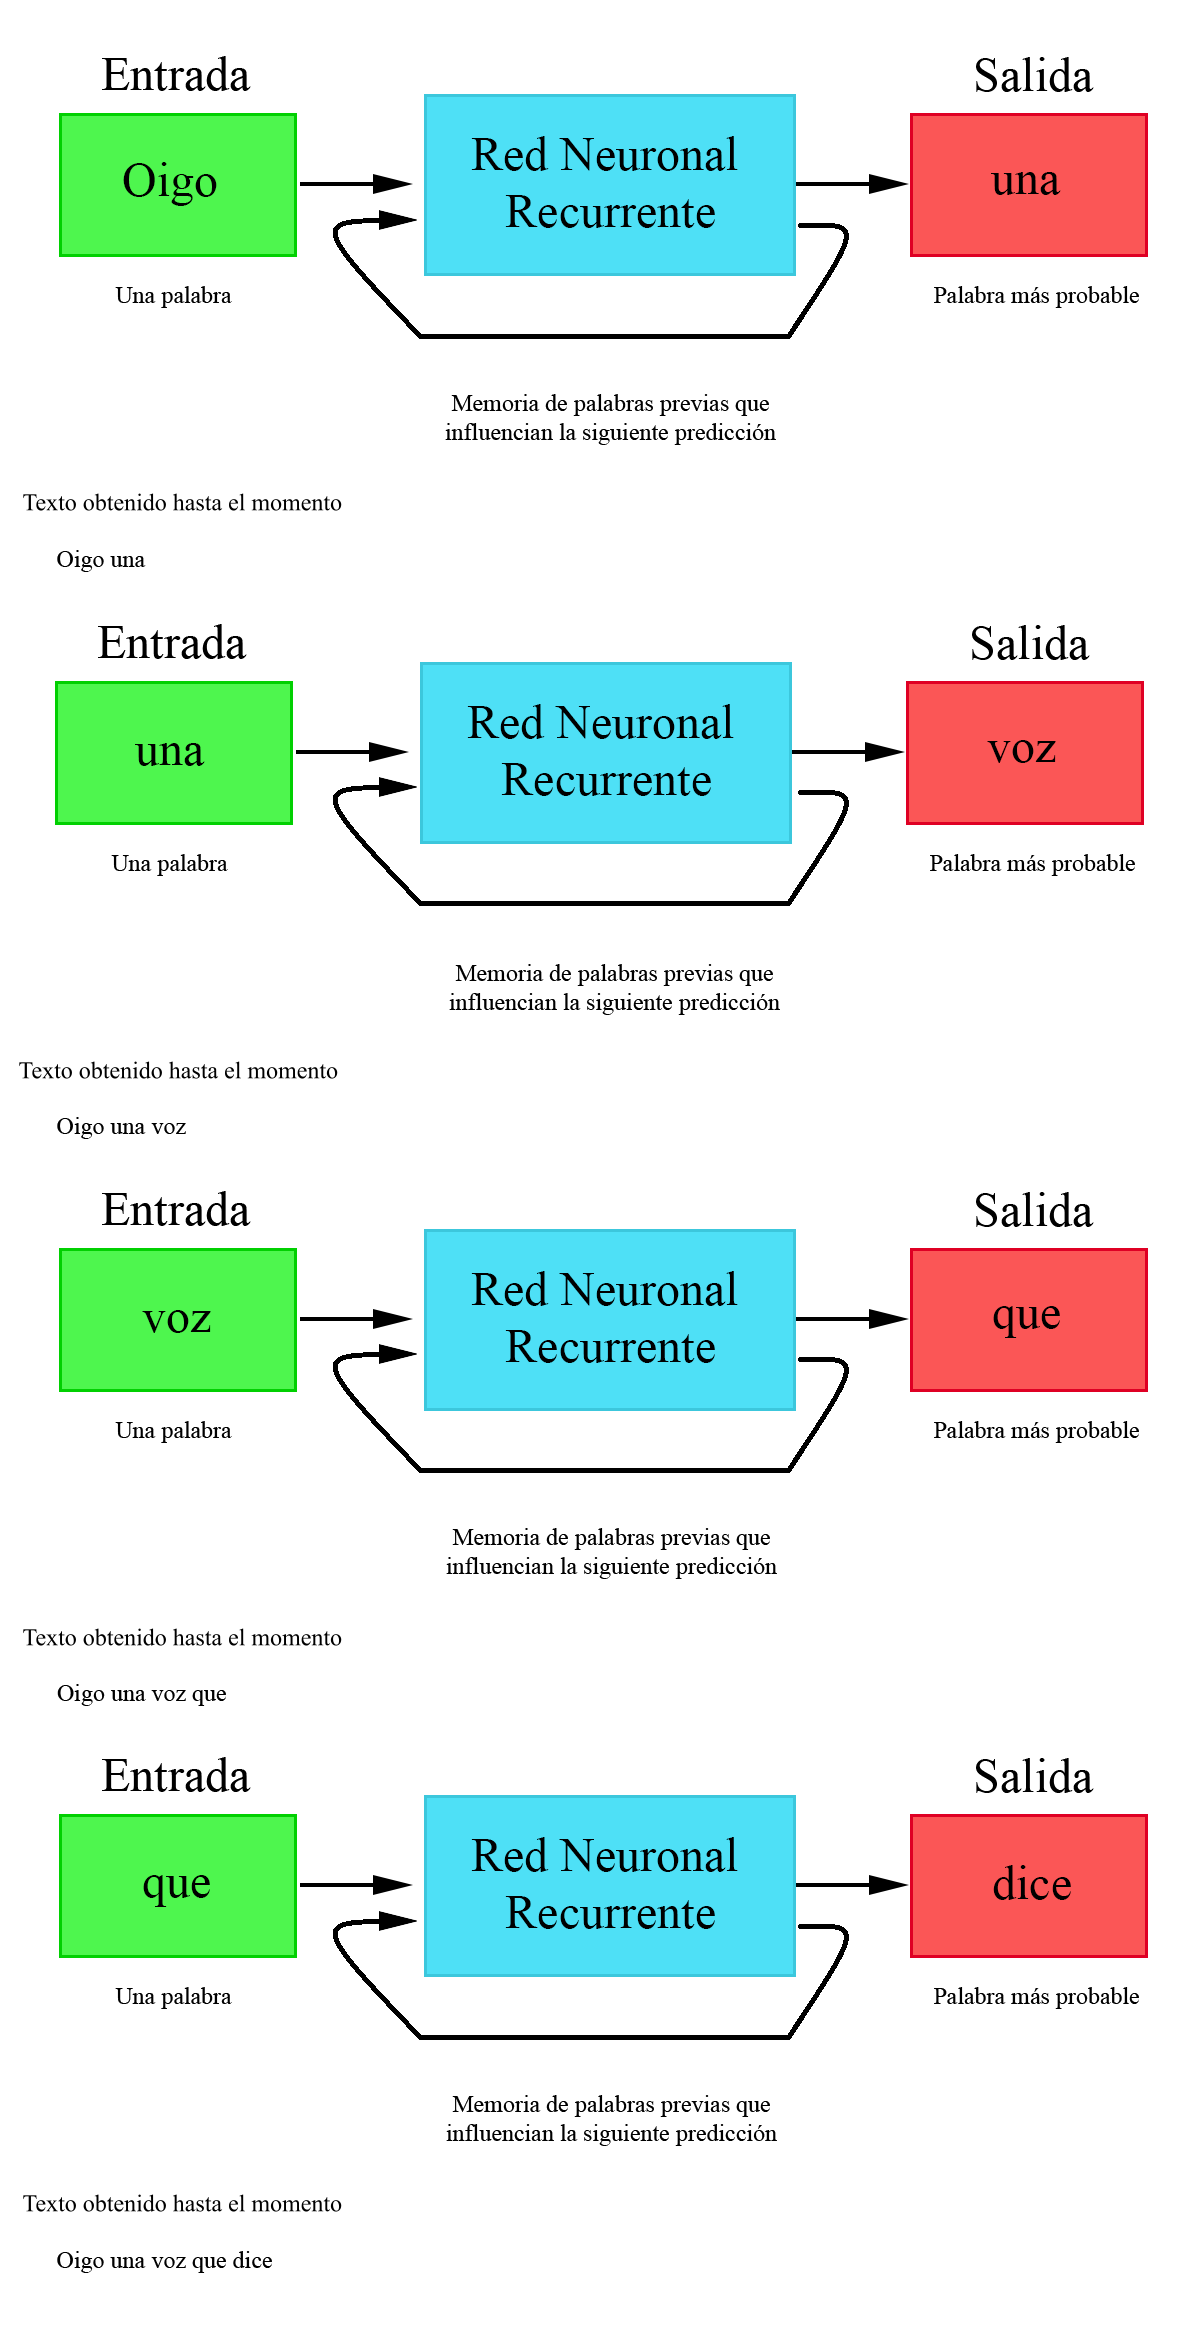
\includegraphics[width=10cm]{./imagenes/MarcoTeorico/RedesN/Recurrente.png}
					\centering 
					\caption{Diagrama de una red neuronal recurrente}
				\end{figure}		
        
        \section{Procesamiento de lenguaje natural}
        
        El \acrfull{pln} se refiere a una rama de la informática, específicamente, a una rama de la inteligencia artificial, la cual se ocupa de dar a las computadoras la capacidad de comprender texto y palabras de la misma manera que los seres humanos.\\\\
        El \acrshort{pln} combina la lingüística computacional con modelos estadísticos, machine y deep learning. Juntas, estas tecnologías permiten a las computadoras procesar el lenguaje humano en forma de texto o datos de voz y `comprender' su significado completo, es decir, la intención y el sentimiento del hablante o escritor. \cite{refProcesamientoLN}
        
		        \subsection{Tareas del procesamiento de lenguaje natural}
		        \begin{itemize}
		        	\item \textbf{Reconocimiento de voz: }Su tarea pertinente es la conversión de voz a texto, requiere convertir de manera confiable datos de voz en datos de texto. Lo cual hace al reconocimiento de voz una tarea especialmente desafiante es la forma en que las personas hablan: velocidad, arrastrando las palabras, con diferentes énfasis, entonación y acentos.
		        	\item \textbf{Etiquetado de palabras: }Es el proceso de determinar la parte gramatical de una palabra o fragmento de texto en particular, en función de su uso y contexto.
		        	\item \textbf{Desambiguación de las palabras: }Es la selección del significado de una palabra con múltiples significados a través de un proceso de análisis semántico que determina la palabra que tiene más sentido en el contexto dado. 
		        	\item \textbf{Reconocimiento de entidad nombrada: }Identifica palabras o frases como entidades útiles, es decir, identifica nombres propios.
		        	\item \textbf{Resolución de correferencia: }Es la tarea de identificar si dos palabras se refieren a la misma entidad. El ejemplo más común es determinar la persona u objeto al que se refiere un determinado pronombre.
		        	\item \textbf{Análisis de sentimientos: }Intenta extraer del texto cualidades subjetivas (actitudes, emociones, sarcasmo, confusión, sospecha).
		        	\item \textbf{Generación de lenguaje natural: }Es la tarea de convertir información estructurada a lenguaje humano.
		        \end{itemize} 
		    
		    	\subsection{Usos del procesamiento de lenguaje natural}
		    	
		    	El procesamiento del lenguaje natural es el cerebro detrás de la inteligencia artificial en muchas aplicaciones del mundo real. Algunos ejemplos son los siguientes:
		    	
		    	\begin{itemize}
		    		\item \textbf{Aplicaciones dedicadas a la traducción: }un ejemplo de estos es Google Translate, el cual hace uso de \acrshort{bert} para el procesamiento del lenguaje natural así como para el etiquetado de las palabras que requiere traducir.
		    		\item \textbf{Asistentes virtuales y chatbots: } Existen hoy en día diferentes tecnologías que simulan ser asistentes virtuales como Siri o Alexa requieren de un reconocimiento de voz para distinguir comandos, así como para responder adecuadamente a estos. En el caso de los chatbots realizan un análisis contextual de las preguntas para proveer respuestas relacionadas a las mismas.
		    		\item \textbf{Análisis de sentimientos en redes sociales: }Consta de analizar el lenguaje utilizado en publicaciones dentro de las redes sociales, respuestas, reseñas y más para extraer actitudes y emociones en respuesta a productos, promociones y eventos; información que las empresas pueden usar en diseños de productos, campañas publicitarias y más
		    		\item \textbf{Resúmenes de textos: }Consta de realizar resúmenes y sinopsis de distintos textos.
		    	\end{itemize} 
        
        \section{Transformers}
        El Transformer en \acrfull{pln} es una arquitectura que tiene como objetivo codificar cada palabra que compone una frase en función a la secuencia que cada palabra sigue, permitiendo así agregar un contexto o una representación matemática dentro del texto.\\\\    
        Se suele trabajar con los transformadores en dos etapas: 
        \begin{itemize}
        	\item \textbf{Pre-entrenamiento: }En esta etapa, el modelo aprende cómo se estructura el lenguaje de forma general, así como de obtener un conocimiento general del significado de las palabras dentro de la frase trabajada.\cite{refQueesuntransformer}
        	\item \textbf{Afinado: }En esta etapa se añaden ciertas capas o funciones a la arquitectura para adaptar los modelos y que estos realicen ciertas tareas, para después estos modelos ser re-entrenados y cumplan con las tareas establecidas de manera correcta.\cite{refQueesuntransformer}
        \end{itemize}  
   
		   		\subsection{Arquitectura de un transformer} 
		   		
		   		\begin{figure}[H] 
		   			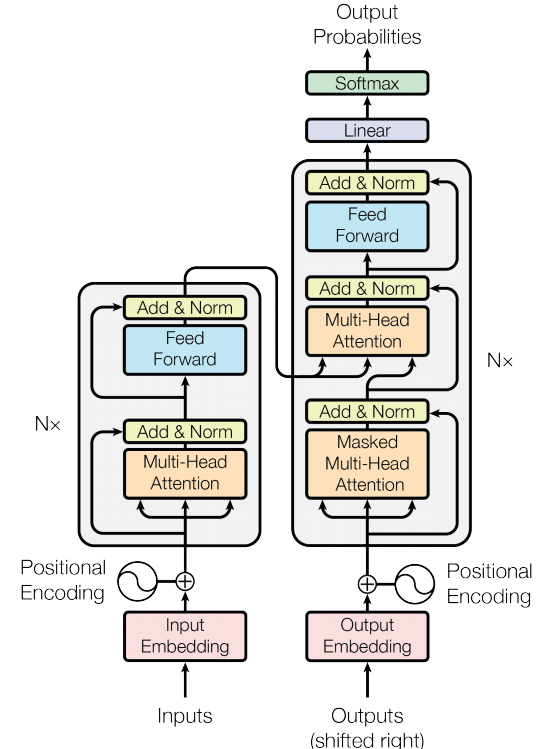
\includegraphics[width=12cm]{./imagenes/MarcoTeorico/Transformerarchitecture.png}\label{ArqTransformer}
		   			\centering 
		   			\caption{Arquitectura general de un transformer \cite{refArqTransformer}}
		   		\end{figure}     
		        El codificador mapea una secuencia de entrada las cuales son representaciones de símbolos (x1, ..., xn) a una secuencia de representaciones continuas z = (z1, ..., zn). Dado z, el decodificador genera una salida secuencia (y1, ..., ym) de símbolos, un elemento a la vez. En cada paso, el modelo es autor-regresivo, consumiendo los símbolos generados previamente como entrada adicional para generar el siguiente.\\\\
		        Los transformers siguen esta arquitectura general usando auto-atención, es decir, las capas están completamente conectadas tanto para el codificador como para el decodificador, que se muestran en las mitades izquierda y derecha de la Figura 2.4 anterior, respectivamente. \cite{refArqTransformer}
        
        \section{\acrshort{bert}}
		        \subsection{¿Qué es BERT?}
		        \acrfull{bert} es un marco de aprendizaje automático de código abierto para el \acrfull{pln}. \acrshort{bert}, significa representaciones de codificador bidireccional de transformers, el cual es un modelo de aprendizaje profundo en el que cada elemento de salida está conectado a cada uno de entrada y las ponderaciones entre ellos se calculan dinámicamente en función de su conexión. \cite{refQueesBert} \\\\        
		        Al contar con la capacidad bidireccional, \acrshort{bert} está previamente entrenado en dos tareas de \acrshort{pln} diferentes, pero relacionadas: el modelado de lenguaje enmascarado y la predicción de la siguiente oración.\\\\        
		        El objetivo del entrenamiento \acrfull{mlm} es ocultar una palabra en cada oración y luego hacer que el programa prediga qué palabra se ha ocultado en función del contexto de la que esta oculta. El objetivo del entrenamiento de predicción de la siguiente oración es que el programa prediga si dos oraciones dadas tienen una conexión lógica secuencial o si su relación es simplemente aleatoria.\\\\
		        
		        \subsection{¿Cómo funciona \acrshort{bert}?}
		        
		        El objetivo de cualquier técnica utilizando \acrshort{pln} es comprender el lenguaje humano tal como se habla de forma natural. En el caso de \acrshort{bert}, esto normalmente significa predecir la siguiente palabra. Para hacer esto, los modelos normalmente necesitan entrenarse usando un gran repositorio de datos para usarlos en el entrenamiento, los cuales estarán especializados y etiquetados.\\\\     
		        \acrshort{bert}, sin embargo, fue entrenado previamente usando solo un corpus de texto plano sin etiquetar (textos de Wikipedia en inglés). Continúa aprendiendo sin supervisión del texto sin etiquetar y mejorando incluso cuando se usa en aplicaciones prácticas. Su entrenamiento previo sirve como una capa base de “conocimiento”. A partir de ahí, \acrshort{bert} puede adaptarse al creciente cuerpo de contenido y consultas para ajustarse a las especificaciones del usuario. Este proceso se conoce como aprendizaje por transferencia.\\\\        
		        \acrshort{bert} es posible gracias a la investigación de Google sobre transformers. El transformer es la parte del modelo que le da a \acrshort{bert} su mayor capacidad para comprender el contexto y la ambigüedad en el lenguaje. Se hace esto procesando cualquier palabra dada en relación con todas las demás palabras en una oración, en lugar de procesarlas una a la vez.\par        
		        
		        \begin{figure}[H] 
		        	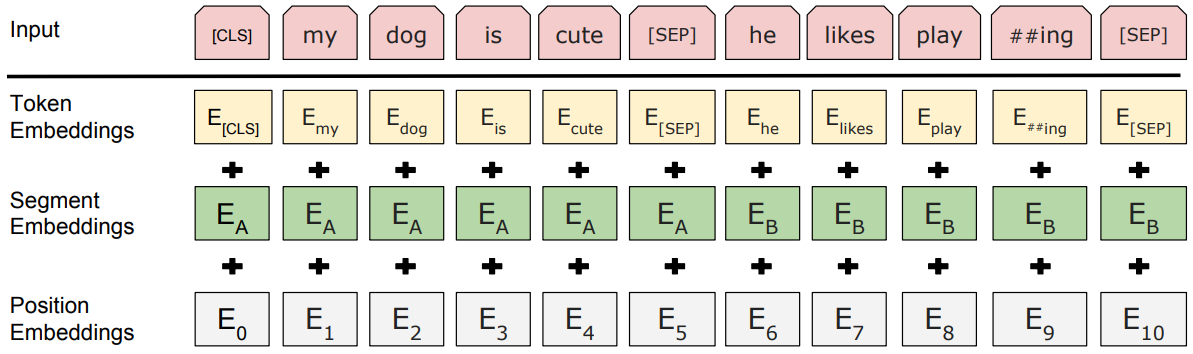
\includegraphics[width=12cm]{./imagenes/MarcoTeorico/Bertprocess.png}
		        	\centering 
		        	\caption{Representación de entrada de \acrshort{bert} y la separación de oración por palabras y la asignación de valores.\cite{refQueesBert}}
		        \end{figure} 
		           
		        En la figura anterior, lo que se realiza es que se inserta un token [\acrfull{cls}] al principio de la primera oración y un token [\acrfull{sep}] al final ella, cada palabra es separada en una ficha, a cada ficha se agrega una inserción que indica si se trata de la oración A o la oración B, finalmente se agrega una incrustación posicional a cada token para indicar su posición en la secuencia. \cite{refComofuncionaBert}\\\\     
		        Esto contrasta con el método tradicional de procesamiento del lenguaje, conocido como incrustación de palabras, en el que los modelos mapeaban cada palabra en un vector, que representa sólo una dimensión, es decir, el significado de esa palabra.\par
		        
		        \subsection{\acrshort{bert} en la actualidad}
		        
		        \acrshort{bert} se utiliza actualmente en Google para optimizar la interpretación de las búsquedas que realizan los usuarios.\\\\
		        Así como en la realización de tareas tales como: \cite{refBertactualidad}
		        \begin{itemize}
		        	\item Generación de lenguaje basadas en secuencia a secuencia (Respuesta a preguntas, resúmenes de documentos, predicción de siguiente oración, chatbots). 
		        	\item Comprensión del lenguaje natural (Entendimiento de la polisemia, correferencia, desambiguación y clasificación de la palabras por sentimientos).
		        \end{itemize}         
       
        \section{GPT-2}
		        \subsection{¿Qué es GPT-2?}  
		        \acrfull{gpt} es un transformer aprovechado para realizar tanto aprendizaje supervisado como no supervisado para el \acrfull{pln}.\\\\        
		        \acrshort{gpt}-2 es el sucesor de \acrshort{gpt}, es un gran modelo de lenguaje basado en transformers con 1500 millones de parámetros, entrenado en un conjunto de datos de 8 millones de páginas web. \acrshort{gpt}-2 se entrena con un objetivo simple: predecir la siguiente palabra, dadas todas las palabras anteriores dentro de un texto. \cite{refQueesgpt}\\\\
		        El conjunto de datos no requiere ningún paso de procesamiento previo. En otras palabras, se omiten las mayúsculas y minúsculas, la tokenización y otros pasos, ya que los autores creen que estos pasos de preprocesamiento restringen la capacidad del modelo y así ser capaz de evaluar todos los puntos de referencia del lenguaje.\\\\        
		        Ya que en \acrshort{gpt}-2 no se aplica una representación de las palabras ni a nivel de palabra ni a nivel de carácter. Se elige una opción que se encuentra situada en medio, que es la subpalabra. La subpalabra se puede obtener mediante el algoritmo \acrfull{bpe}.\\\\
		        \acrshort{bpe} es una forma de compresión donde se calculará una lista de subpalabras utilizando el siguiente algoritmo: \cite{refbpe}
		        \begin{itemize}
		        	\item Dividir palabra en secuencia de caracteres.
		        	\item Unirse al patrón de frecuencia más alta
		        	\item Continuar con el paso anterior hasta alcanzar el número máximo predefinido de subpalabras de iteraciones.
		        \end{itemize}
		    
		    	\subsection{Arquitectura GPT-2}
		    	
		    	\begin{figure}[H] 
		    		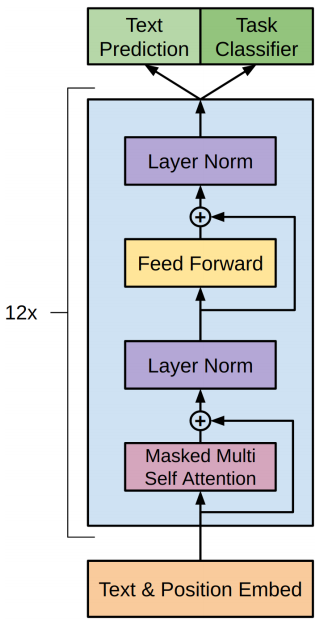
\includegraphics[scale=.5]{./imagenes/MarcoTeorico/GPTransformer.png}
		    		\centering 
		    		\caption{Arquitectura del modelo de \acrshort{gpt}-2 \cite{refarquitecturagpt}}
		    	\end{figure}
		    
		    	El modelo de \acrshort{gpt}-2 es un transformer decodificador de 12 capas, cada una con 12 mecanismos de atención independientes, llamados “cabezas”; el resultado es 12 x 12 = 144 patrones de atención distintos. Cada uno de estos corresponde a una propiedad lingüística capturada por el modelo. \cite{refarquitecturagpt2} \\\\
		    	Lo que le permite identificar la relación que existe entre las palabras, entendiendo la oración y permitiendo predecir la siguiente palabra en relación a la oración.\par
		    	
		    	\begin{figure}[H] 
		    		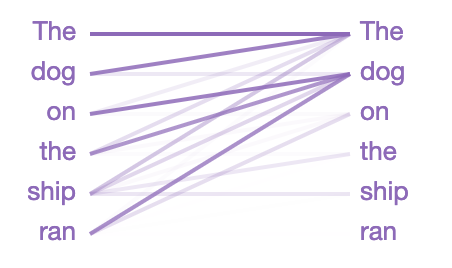
\includegraphics[width=9cm]{./imagenes/MarcoTeorico/Gptsentence.png}
		    		\centering 
		    		\caption{Ejemplo análisis de una oración por \acrshort{gpt}-2 \cite{refarquitecturagpt3}}
		    	\end{figure}
		    
		    	Las líneas, leídas de izquierda a derecha, muestran dónde presta atención el modelo prediciendo la siguiente palabra en la oración (la intensidad del color representa la fuerza de la atención). Entonces, al tratar de predecir la siguiente palabra después de correr (ran), el modelo presta mucha atención al perro (dog) en este caso. Esto ya que necesita saber quién o qué está corriendo para predecir qué viene a continuación. \cite{refarquitecturagpt3}    	
		    	
    	\section{\acrshort{bert} vs GPT-2}    	
    	Dentro de esta sección mostramos una pequeña comparación entre las tecnologías \acrshort{bert} y GPT-2, visualizada en la siguiente tabla:    	
    	\begin{table}[h!]    		
    		\caption[Comparación entre tecnologías BERT y GPT-2]{Comparación entre las tecnologías \acrshort{bert} y GPT-2}
    		\begin{tabular}{|m{6.5cm}|m{6.5cm}|}
    			\hline    			
    			\rowcolor{guindapoli}
    			{\textbf{\textcolor{white}{\acrshort{bert}}}} & {\textbf{\textcolor{white}{\acrshort{gpt}-2}}}\\
    			\hline
    			Es de naturaleza bidireccional. & Es de naturaleza autor-regresivo\\
    			\hline
    			El usuario puede entrenar sus propios modelos. & Puede resolver distintos problemas de \acrfull{pln} sin necesidad volver a entrenar la red neuronal.\\
    			\hline
    			La separación de palabras es manejada en tokens. & La separación de palabras es realizada por medio del algoritmo \acrfull{bpe} generando subpalabras.\\
    			\hline
    			Su uso es enfocado al análisis y generación de textos. & Sus principales usos son para la generación de textos.\\
    			\hline
    		\end{tabular}
    	\end{table}
        Con base en lo anterior se determino que se va a utilizar \acrshort{bert} el resto del trabajo terminal para ayudarnos en la generación de los textos. \pagebreak	
        
        \section{Base de datos}
        
        Una base de datos es un conjunto organizado de datos o información, los cuales pertenecen a un mismo contexto, se encuentran almacenados de forma física o digital con la finalidad de realizar distintas acciones como consultas futuras, ingreso de nuevos datos, actualización o eliminación de estos.\\\\
		Las bases de datos se componen de una o más tablas divididas en columnas y filas, estas son las encargadas de guardar un conjunto de datos.\\\\
		Una base de datos generalmente es manejada por un \acrfull{dbms}. En conjunto, el \acrshort{dbms} y los datos o información, unido a las aplicaciones asociadas a ellos, se les conoce como un sistema de base de datos.\cite{refQueEsBD}\par
			\subsection{Base de datos NoSQL o no relacionales}
			Estas bases permiten que los datos no estructurados y/o semiestructurados se almacenen y manipulen, a diferencia de la base de datos relacional donde se define como deben de componerse todos los datos insertados en esta. Generalmente los registros de este tipo de base de datos suelen almacenarse como un documento de tipo \acrshort{json}.\par
		
		\newpage
		\section{Género musical}
		Un género musical es hablar de una categoría la cual reúne una diversidad de composiciones musicales las cuáles tienen ciertos criterios en común, estos pueden ser su instrumentación, cómo se va a emplear, el contexto en el que son desarrolladas o el contenido de su lírica.
		
			\subsection{Género Pop}
			El género de musical popular o mejor conocido como música pop, se trata de una combinación de otros géneros musicales, este tipo de género trata de ser ecléctico, es decir, trata de reunir ideas, tendencias, valores, etc. Aunque como todo, cuenta con ciertas características que lo diferencían, algunas de estas diferencias son que la duración de las canciones suele ser de corta a media duración, siguen una estructura simple de estrofa-estribillo, la cual consta de un grupo de versos a los cuales le acompañan un pequeño grupo de versos los cuales se repiten, por lo mismo, estás se distinguen por el uso habitual de estribillos repetidos, así como de ganchos los cuales son un pasaje (una melodía) o una frase la cual busca llamar la atención del oyente.
	    
	    \section{Canción}
	    Una canción por definición, es una composición literaria, generalmente escrita en versos, a la cual se le puede acompañar con música para poder ser cantada.\cite{refEstructuraCancion1}\par
			\subsection{Elementos de una canción}
			Los elementos que conforman una canción son los siguientes:

				\subsubsection*{Introducción}\par
				Generalmente es una parte única la cual se encuentra al inicio de una canción, acompañada de una \gls{Armonia} o \gls{Melodia} compuesta solo para este inicio. El objetivo de la introducción es de atraer la atención y producir un ambiente.\cite{refEstructuraCancion2}\par
				\subsubsection*{Verso}\par
				Es la parte encargada de comenzar a desarrollar la idea a transmitir, trata de contarnos el tema de la canción, y ya cuenta con una \gls{Armonia} bien establecida.\par
				\subsubsection*{Pre-coro}\par
				Es un arreglo que permite realizar una transición, su función principal es conectar el verso y coro. También ayuda a evitar que el coro se estanque en la monotonía.\par
				\subsubsection*{Coro}\par
				Es una \gls{Estrofa} la cual se repite varias veces dentro de una composición. Su función principal es acentuar la idea más importante de la canción tanto en su letra como en lo musical. Se considera como una de las partes más importantes dentro de una canción y en algunas ocasiones este es repetido al inicio y final.\par
				\subsubsection*{Puente}\par
				Es un interludio el cual conecta dos fragmentos de una canción, permitiendo construir una \gls{Armonia} entre ellas, suele ser usado para llevar a la canción al clímax, preparándose para el desarrollo final de la canción.\par
				\subsubsection*{Cierre}\par
				Este busca terminar o concluir la pieza musical, una de las formas puede ser un ruptura brusca generada por un silencio imprevisto o por una secuencia de \gls{Acordes}. Pero la manera más ordinaria de cerrar es haciendo uso de la repetición de un coro.\par

			\newpage
			
			\subsection{Estructura de una canción}
			La estructura mínima de una canción está compuesta de:\par
			\begin{itemize}
			  \item Verso
			  \item Coro
			  \item Verso
			  \item Coro
			\end{itemize}\par
			La estructura más empleada en una canción es la siguiente:
			\begin{itemize}
			  \item Introducción
			  \item Verso
			  \item Pre-coro
			  \item Coro
			  \item Verso
			  \item Coro
			  \item Puente
			  \item Cierre
			\end{itemize}
		
			Se pretende trabajar la estructura de la generación de letras musicales de la siguiente forma:
			
			\begin{figure}[H] 
				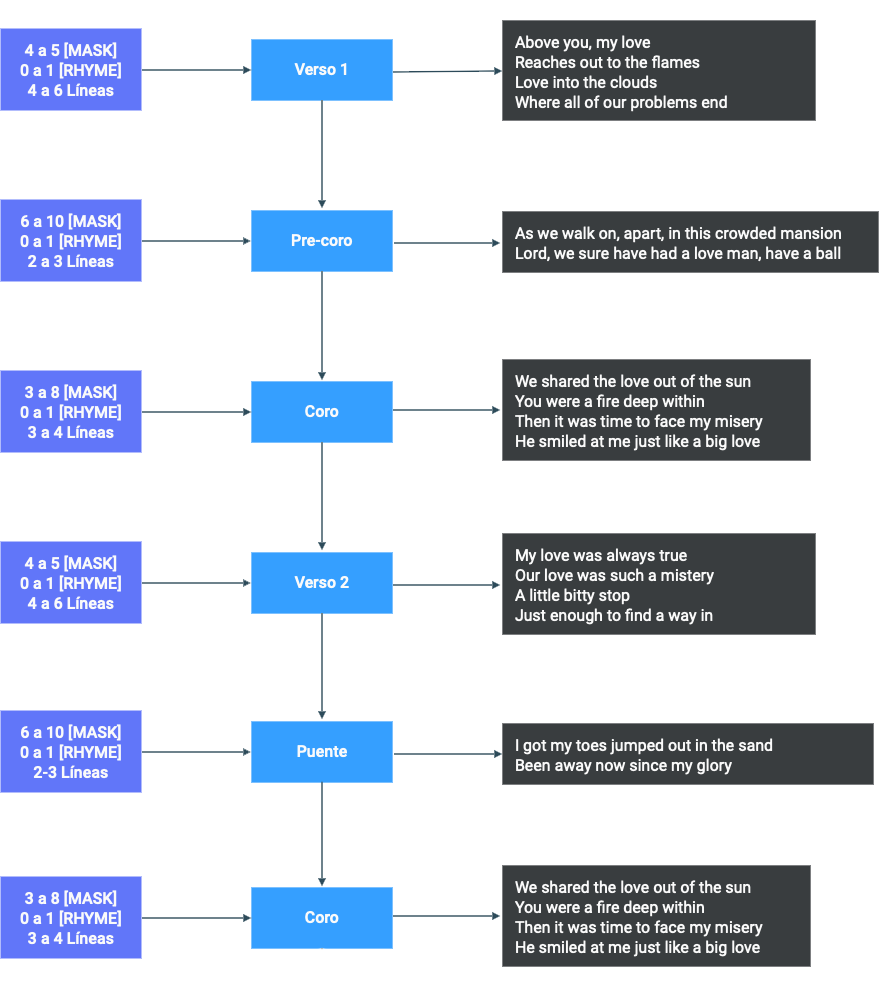
\includegraphics[scale=.45]{./imagenes/Disenio/Arquitectura/Generacion_letras.png}
				\centering 
				\caption{Diagrama de la estructura para la generación de las letras musicales}
			\end{figure}
		
		\newpage
		
		\section{Cadenas de Markov}
	    Las cadenas de Markov son un \gls{Sistema} matemático el cual experimenta con las transiciones de un \gls{Estado} a otro de acuerdo con ciertas reglas probabilísticas. La característica que define a una cadena de Markov es que no importa cómo llegó el proceso a su estado actual, y sus posibles estados futuros son fijos. En otras palabras, la probabilidad de pasar a cualquier otro estado depende únicamente del estado actual y del tiempo transcurrido. El espacio de estados o conjunto de todos los posibles estados, pueden ser cualquier cosa: letras, números, puntuaciones de un partido, acciones, etc.\\\\
		Son procesos \gls{Estocastico}s, con la diferencia de que estos deben ser “sin memoria”, es decir, la probabilidad de las acciones futuras no depende ni se ve afectada de los pasos que la condujeron al estado actual. A esto se le denomina una propiedad de Markov.\\\\
		En la teoría de probabilidad, el ejemplo más inmediato es el de una cadena de Markov homogénea en el tiempo, en la que la probabilidad de que ocurra cualquier transición de estado es independiente del tiempo.\\\\
		En el lenguaje de probabilidad condicional y variables aleatorias, una cadena de Markov es una secuencia X0, X1, X2, … de variables aleatorias que satisfacen la regla de independencia condicional.
		En otras palabras, el conocimiento del estado anterior es todo lo que se necesita para determinar la distribución de probabilidad del estado actual. Esta definición es más amplia que la explorada anteriormente, ya que permite probabilidades de transición no estacionarias y, por lo tanto, cadenas de Markov no homogéneas en el tiempo; es decir, a medida que pasa el tiempo los pasos aumentan y la probabilidad de pasar de un estado a otro puede cambiar. \cite{refMarkov}\\\\
		Las cadenas de Markov pueden ser modeladas mediante \gls{Maquinas de Estados Finitos}.\par
		\begin{figure}[H]
			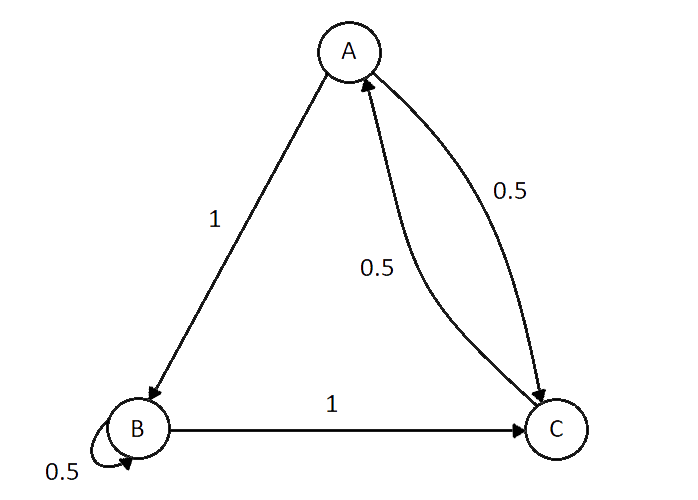
\includegraphics[width=12cm]{./imagenes/MarcoTeorico/Markov/CMarkov.png}
			\centering 
			\caption{Diagrama de estados finitos de una cadena de Markov \cite{refMarkov}}
		\end{figure}
		\begin{comment}
		\section{Flask}
		Flask es un “micro” marco (framework) el cual nos permite crear de manera sencilla aplicaciones web utilizando Python, bajo el patrón de arquitectura \acrfull{mvc}; cabe mencionar que soporta otros lenguajes como PHP y Java.\cite{refFlask}\\\\
		No cuenta con un Manejador de Objetos Relacionales u \acrshort{orm} por sus siglas en inglés, pero si cuenta con características como el enrutamiento de \acrshort{url}S y un motor de plantillas. Flask solo nos da las herramientas necesarias para poder crear una aplicación web funcional, pero si se requieren de otras herramientas para añadir alguna funcionalidad, se puede adaptar añadiéndole ciertos plugins.\\\\
		En general es un marco de aplicación web \acrshort{wsgi}. \acrfull{wsgi} es una especificación que describe como se va a comunicar un servidor web con una aplicación web, y como se pueden llegar a enlazar distintas aplicaciones web para procesar una solicitud o una petición.\\\\		
		\end{comment}
	    \section{Apache}
	    
	 	Es un servidor web gratuito y de código abierto el cual permite que los desarrolladores de sitios web puedan desplegar el contenido de ellas, este no es un servidor que se encuentre físicamente, sino que se trata de un software el cual ejecuta un servidor. Su función es instaurar la conexión entre un servidor y los usuarios del sitio web mientras estos intercambian archivos entre ellos (siguiendo una estructura cliente-servidor). El servidor y cliente interactúan mediante el protocolo \acrshort{http}, y el software de Apache es el encargado de mantener una comunicación ágil y segura entre las 2 partes.\cite{Apache}\\\\
	 	Apache trabaja sin problemas con otros sistemas de gestión de contenido (Drupal, Joomla, etc.), marcos de trabajo (Django, Laravel, etc.), y lenguajes de programación. Por estas razones se vuelve una opción sólida al momento de escoger entre los distintos tipos de plataformas de alojamiento web, como serían \acrfull{vps} o alojamiento compartido.\cite{what_is_apache}\\
		\begin{comment}
		\section{NGINX}
		
		NGINX es un software de código abierto para servicio web, almacenamiento en caché, equilibrio de carga, proxy inverso, transmisión de medios y más. Inició como un servidor web diseñado para un máximo rendimiento y estabilidad. Además de sus capacidades de servidor \acrshort{http}, NGINX también puede funcionar como un servidor proxy para correo electrónico (\acrshort[IMAP], \acrshort[POP] y \acrshort[SMTP]) y un proxy inverso, así como un equilibrador de carga para servidores \acrshort{http}, \acrshort[TCP] y \acrshort[UDP].\cite{refNginx}\\
		\end{comment}
		\newpage
			
		\begin{table}[hbt!]
			\caption[Comparación de servidores web]{Tabla comparativa de los distintos servidores web contemplados para nuestro proyecto}
			\begin{tabular}{|m{7.5cm}|m{7.5cm}|}
				\hline 	
				\rowcolor{guindapoli}
				{\textbf{\textcolor{white}{Apache}}} & {\textbf{\textcolor{white}{NGINX \cite{refNginx}}}}\\
				\hline
				Es fácil de configurar, cuenta con muchos módulos, así como un entorno sencillo. & Usa hilos para manejar solicitudes del usuario.\\
				\hline
				De código abierto y gratuito, inclusive si se usa de manera comercial. & Nginx es uno de los servidores web que soluciona el problema c10k y seguramente de los más exitoso al hacerlo.\\
				\hline
				Software estable y confiable. & No crea un nuevo proceso por cada solicitud.\\
				\hline
				Frecuentemente actualizado incluyendo actualizaciones regulares a los parches de seguridad. & Maneja toda solicitud entrante en un único hilo.\\
				\hline
				Funciona de forma intuitiva, con sitios web hechos con WordPress.  & El modelo basado en eventos de Nginx reparte las solicitudes de los usuarios entre procesos de trabajo de manera eficiente.\\
				\hline
				Comunidad grande y posibilidad de contactar con soporte disponible de manera sencilla en caso de cualquier problema. &  Cuenta con mejor escalabilidad.\\
				\hline
				Presenta inconvenientes de rendimiento con sitios web los cuales tienen alto tráfico. & Es capaz de manejar un sitio web con demasiado tráfico con un uso de recursos mínimo.\\
				\hline
				Al contar con muchas preferencias de configuración puede generar vulnerabilidades de seguridad. & \\
				\hline	
			\end{tabular}
		\end{table}
		En ambos casos, se mantienen en desarrollo, con actualizaciones constantes, así como frecuentemente sacando parches para evitar ataques de DDos.
	    \section{Servidor web}
	        La función es mostrar sitios web en internet. A fin de conseguir este objetivo, actúa como un mediador entre el servidor y el dispositivo del cliente. Obtiene el contenido del servidor en cada petición hecha por el usuario y lo entrega al sitio web.\cite{What_is_a_web_server}\\\\
	        Los servidores web son capaces de procesar archivos escritos en distintos lenguajes de programación como Java, PHP, Python, y otros.\\\\
	        Podría decirse que un servidor web es la herramienta responsable por la correcta comunicación entre el cliente y el servidor.

		 \section{Certificado SSL}
			Conocido como \acrfull{ssl} o (Capa de Conexión Segura) es un estándar de seguridad global que fue originalmente creado por Netscape en los 90's. \acrshort{ssl} crea una conexión encriptada entre tu servidor web y el navegador web de tu visitante permitiendo que la información privada sea transmitida sin que ocurran problemas como serían espionaje, manipulación de la información, y falsificación de los datos del mensaje.\cite{what_is_SSL} Básicamente, la capa \acrshort{ssl} permite que dos partes tengan una “conversación” privada.\\\\
			Para establecer esta conexión segura, se instala en un servidor web un certificado \acrshort{ssl} (también llamado `certificado digital') que cumple dos funciones:
			
			\begin{itemize}
				\item Autentificar la identidad del sitio web, garantizando a los visitantes que no están en un sitio falso. 
				\item Cifrar la información transmitida.
			\end{itemize}
		
			Hay varios tipos de certificados \acrshort{ssl} \cite{ssl_certificates} según la cantidad de nombres de dominio o subdominios que se tengan, como por ejemplo:
			
			\begin{itemize}
				\item Único: Asegura un nombre de dominio o subdominio completo (\acrfull{fqdn} por sus siglas en inglés). 
				\item Comodín: Cubre un nombre de dominio y un número ilimitado de sus subdominios.
				\item Multidominio: Asegura varios nombres de dominio.
			\end{itemize}
		
		\newpage
		\section{Plataformas en la nube para generar modelos de aprendizaje automático}
		
		El entrenamiento de aprendizaje automático y de modelos de aprendizaje profundo involucra miles de iteraciones. Se necesitan esta gran cantidad de iteraciones para producir el modelo más preciso.\\\\ 
		El cómputo en la nube permite modelar capacidad de almacenamiento y manejar cargas a escala \cite{data_science_in_the_cloud}, o escalar el procesamiento a través de los nodos. Por ejemplo, \acrshort{aws} ofrece instancias de \acrshort{gpu}s con capacidad de memoria que va de los 8Gb's a los 256Gb's, estas instancias son cobradas a ritmos por hora.\\\\
		Las \acrshort{gpu}s son procesadores especializados diseñados para procesado complejo de imágenes. Azure de Microsoft ofrece \acrshort{gpu}s de alto rendimiento de la serie NC para aplicaciones o algoritmos de cómputo de alto rendimiento.
		
				\subsection{Amazon Web Services}
				Dentro de las bondades que ofrecen los Servicios Web de Amazon (\acrfull{aws} por sus siglas en inglés) y que nos pueden ser de utilidad para las nacesidades de nuestro proyecto se pueden encontrar: 
				
				\begin{itemize}
					\item \textbf{SageMaker:} Es una plataforma de aprendizaje automático completamente administrado para científicos de datos y desarrolladores. La plataforma corre en Cómputo Elástico en la Nube (\acrfull{ec2} por sus siglas en inglés), y permite construir modelos de aprendizaje automático, organizar la información y escalar sus operaciones. \\
					Algunas aplicaciones de aprendizaje automático en SageMaker van desde reconocimiento de voz hasta visión de computadora, e incluso recomendaciones basadas en el comportamiento aprendido del usuario.\\\\ 
					El mercado de \acrshort{aws} ofrece modelos que se pueden usar en lugar de empezar desde cero, posterior a eso se puede entonces empezar a entrenar y optimizar el modelo; las elecciones más comunes son frameworks como Keras, TensorFlow, y PyTorch; Sagemaker puede optimizar y configurar estos frameworks automáticamente, o pueden ser entrenadas de manera personal.\\\\ 
					\newpage
					Uno mismo puede incluso desarrollar su propio algoritmo construyéndolo en un contenedor de Docker o se puede hacer uso de una “Jupyter notebook” \cite{what_is_jupyter} para construir un modelo propio de aprendizaje automático y visualizar su información usada para el entrenamiento del modelo siendo este punto lo que más nos interesa para nuestro proyecto.
					
				\end{itemize}
		
		\begin{comment}
				
					\item \textbf{Lex:} Fue diseñado para integrar chatbots en aplicaciones. Lex cuenta con capacidades de aprendizaje profundo basado en procesamiento de lenguaje natural (PLN) y reconocimiento automático de voz. La API puede reconocer texto hablado y escrito. 
					\item \textbf{Rekognition:} Es un servicio de visión computacional que simplifica el proceso de desarrollo para aplicaciones de reconocimiento de imagen y vídeo.
		
			\subsection{Azure}
			Comparado a AWS, las propuestas del aprendiza de máquina de Azure son más flexibles en términos de algoritmos out-of-the-box.
			
			\begin{itemize}
			\item \textbf{Servicios de Aprendizaje Automático:} Es una gran librería de algoritmos de aprendizaje automático pre-entrenados y pre-empacados, también provee de un ambiente para implementar estos algoritmos y aplicarlos a aplicaciones del mundo real. Se puede usar la interfaz de usuario para entrenar, probar y evaluar los modelos así como también provee soluciones para Inteligencia Artificial (IA) (Esto incluye visualización y otra información que puede ayudar a comprender el comportamiento del modelo y comparar algoritmos para encontrar la mejor opción). Algunas de las ofertas dentro de este apartado son:
			
			\begin{itemize}
			\item \textbf{Paquetes de Python:} Contiene funciones y librerías para visión computacional, análisis de texto, previsión, y aceleramiento de hardware. 
			\item \textbf{Gestión de Modelo:} Provee un entorno para acoger modelos, gestionar versiones, y monitorear modelos que corran en Azure o en soluciones propias de la casa.
			\item \textbf{Workbench:} Una simple línea de comandos y entorno de escritorio con dashboards y herramientas de seguimiento del desarrollo de modelos. 
			\end{itemize}
			
			\item \textbf{Frameworks de Servicio de Bots:} Provee de un entorno para la construcción, despliegue, y prueba  de bots usando diferentes lenguajes de programación.
			\end{itemize}
			
			\subsection{Google}
			Google provee servicios de aprendizaje automático e Inteligencia Artificial (IA) en dos niveles – Motor de Aprendizaje automático de Google Cloud para profesionales de datos experimentados y la plataforma para principiantes de Cloud AutoML (Aprendizaje Automático-Automático).
			
			\begin{itemize}
			\item \textbf{AutoML:} Una plataforma de aprendizaje automático basada en la nube desarrollada para usuarios sin experiencia. Se pueden cargar datasets, entrenar modelos, y desplegarlos en un sitio web. AutoML se integra con todos los servicios de Google y guarda la información en la nube.\\
			Se pueden desplegar modelos entrenados vía una interfaz de REST API. Se puede acceder a un cierto número de productos AutoML disponibles a través de una interfaz gráfica.
			\item \textbf{Motor de Aprendizaje Automático:} Se puede usar Google Cloud ML para entrenar un modelo complejo apalancando la infraestructura de la GPU y la Unidad de Procesamiento de Tensor (TPU por sus siglas en inglés). Incluso se puede usar el servicio para desplegar un modelo entrenado de manera externa.\\
			El Aprendizaje automático en la Nube automatiza todo el monitoreo y los procesos proveedores de recursos para ejecutar las tareas;  aparte de hospedar y entrenar, Cloud ML también puede llevar a cabo ajustes de hiperparámetros que influencian la precisión de las predicciones.
			\item \textbf{Tensorflow:} Es una librería de software open-source que usa gráficas de flujo de datos para operaciones numéricas. Las operaciones matemáticas en estas gráficas son representados por nodos, mientras que los bordes representan la información transferida de un nodo a otro. La información en TensorFlow es representada en forma de tensores, los cuales son arreglos multidimensionales.\\ TensorFlow es usualmente usado para investigación y práctica de aprendizaje profundo, y es multi-plataforma por lo que se puede correr en GPU\'s, CPU\'s, TPU\'s y plataformas móviles.
			\end{itemize}
		\end{comment}
		
		\begin{table}[hbt!]\caption{Tabla comparativa de las diversas plataformas contempladas}% title of Table
			\centering % used for centering table
			\resizebox{15cm}{!} {
				\begin{tabular}{c c c c}% centered columns (3 columns)
					\hline\hline                        %inserts double horizontal lines
					Característica & \acrshort{gcp} \cite{refGoogleCloudPlatform} & \acrshort{aws} \cite{refAmazonWebServices} & Azure \cite{refAzure} \\ [0.5ex]% inserts table %heading
					\hline                  % inserts single horizontal line
					\begin{tabular}[c]{@{}l@{}}Jupyter Notebook\\alojado de \\manera local\\ o remota\\\end{tabular}
					& \begin{tabular}[c]{@{}l@{}}Plataforma de IA\end{tabular}
					& \begin{tabular}[c]{@{}l@{}}SageMaker Studio IDE\end{tabular}
					& \begin{tabular}[c]{@{}l@{}}- Estudio de Notebooks\\ de Azure de Aprendizaje\\ Automático\\- Databrick de Azure\end{tabular} \\% inserting body of the table 
					\hline
					Entrenamiento\\Distribuido
					& \begin{tabular}[c]{@{}l@{}}Si\end{tabular}
					& \begin{tabular}[c]{@{}l@{}}Si\end{tabular}
					& \begin{tabular}[c]{@{}l@{}}Si\end{tabular}\\
					\hline
					Versionado de Modelos
					& Si
					& \begin{tabular}[c]{@{}l@{}}Si\end{tabular}
					& \begin{tabular}[c]{@{}l@{}}Si\end{tabular}\\
					\hline
					Seguimiento de \\Experimentos
					& \begin{tabular}[c]{@{}l@{}}Si\end{tabular}
					& Si
					& \begin{tabular}[c]{@{}l@{}}Si\end{tabular}\\
					\hline
					AutoML\\(\acrshort{ui} y \acrshort{api}) 
					& \begin{tabular}[c]{@{}l@{}}Tabla de AutoML\end{tabular}
					& \begin{tabular}[c]{@{}l@{}}Auto-piloto de\\SageMaker\end{tabular}
					& \begin{tabular}[c]{@{}l@{}}AutoML\end{tabular}\\
					\hline
					Análisis de Errores
					& \begin{tabular}[c]{@{}l@{}}Tabla de AutoML\\con BigQuery\end{tabular}
					& \begin{tabular}[c]{@{}l@{}}Debugger de\\SageMaker\end{tabular}
					& \begin{tabular}[c]{@{}l@{}}Aprendizaje Profundo\\de Azure\end{tabular}\\
					[1ex] % [1ex] adds vertical space
				\end{tabular}\label{table:VentajasServidor}% is used to refer this table in the text
			}
		\end{table}
	
		\newpage
			La tabla anterior se ha basado en la investigación de otras comparaciones en línea \cite{comparing-google-cloud-platform-aws-and-azure} y se ha visto que los tres proveedores de han alojado servicios de “Jupyter Notebook” (contienen tanto código de computadora como elementos ricos en texto como ecuaciones, figuras, etc.), experimentando seguimientos y control de versiones, y métodos de despliegue sencillos.\\
		\\
		Dentro de las características únicas de cada una de las plataformas podemos encontrar que la Plataforma en la Nube de Google (\acrshort{gcp}) usa un paquete llamado “what if tool” el cual se puede integrar junto a un “Jupyter Notebook” y de esa manera jugar con el modelo cambiando el umbral o un valor característico de un ejemplo dado, esto permite checar como es que ciertos cambios afectan el resultado predicho con anterioridad previo al cambio.\\
		\\
		El debbuger de SageMaker de \acrshort{aws} permite analizar cómo es que la ingeniería de características y el refinado del modelo son hechos, o de forma más concisa, permite ver qué sucede durante el entrenamiento del modelo.\\
		\\
		Azure, por su parte, provee un módulo propio en su \acrshort{sdk} el cual parece tener la mejor integración de entre las tres plataformas.\\
		\\
		\textbf{Costo y Rendimiento del Modelo}\\
		\\
		Azure y \acrshort{gcp} puntúan ligeramente mejor que \acrshort{aws} en términos de rendimiento, esto no necesariamente significa que una plataforma es mejor que otra.\\
		\\
		El costo de \acrshort{aws} fue considerablemente menor que \acrshort{gcp} y Azure. Por supuesto, cada una tiene sus fuertes como puede verse en la tabla presentada anteriormente.\\
		\\
		El diseñador de aprendizaje automático de Azure cuenta con una interfaz de arrastar y soltar el cual es bastante amigable con un usuario novato, esto es, porque requiere menos codeo y antecedentes técnicos. \acrshort{aws} y \acrshort{gcp} parecen ser más enfocados a desarrolladores aunque puede resultar en más de trabajo ensamblar una cadena de procesos (pipeline), estos resultan más personalizables con los diferentes componentes disponibles. Estos componentes y la conexión de la cadena de procesos son usualmente desarrollados usando código y configuraciones, en vez de utilizar una interfaz.\\
		\\
		Tanto \acrshort{gcp} como \acrshort{aws} ofrecen un modelo de pago “pay-as-you-go”. Este modelo es el mejor para aquellos individuos que puedan llegar a esperar un uso intermitente de la nube, ya que permite un enfoque flexible para añadir y remover servicios cuando se necesite. Por supuesto, este nivel de flexibilidad tiene un costo, haciendo al modelo “pay-as-you-go” el más caro por hora.
		
		\begin{table}[hbt!]\caption{Tabla comparativa \acrshort{gcp} vs \acrshort{aws}}% title of Table
			\centering % used for centering table
			\resizebox{13cm}{!} {
				\begin{tabular}{c c c}% centered columns (3 columns)
					\hline\hline                        %inserts double horizontal lines
					Tipo de Instancia & Precio de \acrshort{ec2} (por hora) & Precio de Google (por hora) \\ [0.5ex]% inserts table %heading
					\hline                  % inserts single horizontal line
					\begin{tabular}[c]{@{}l@{}}Propósito\\General\end{tabular}
					& \begin{tabular}[c]{@{}l@{}}\$0.134\end{tabular}
					& \begin{tabular}[c]{@{}l@{}}\$0.15\end{tabular} \\% inserting body of the table 
					\hline
					Cómputo\\Optimizado
					& \begin{tabular}[c]{@{}l@{}}\$0.136\end{tabular}
					& \begin{tabular}[c]{@{}l@{}}\$0.188\end{tabular}\\
					\hline
					Optimizado de\\Memoria
					& \begin{tabular}[c]{@{}l@{}}\$0.201\end{tabular}
					& \begin{tabular}[c]{@{}l@{}}\$0.295\end{tabular}\\
					\hline
					\acrshort{gpu}
					& \begin{tabular}[c]{@{}l@{}}\$0.526\end{tabular}
					& \begin{tabular}[c]{@{}l@{}}\$1.4\end{tabular}\\
					[1ex]      % [1ex] adds vertical space
				\end{tabular}\label{table:ComparacionPlataformas}% is used to refer this table in the text
			}
		\end{table}
		La tabla mostrada anteriormente cabe destacar que es en dólares estadounidenses y se utilizó una comparación hecha en otro artículo. \cite{google_cloud_vs_aws}
		En conclusión, la opción ideal para las necesidades de nuestro proyecto es \acrshort{aws} debido a que es más económico que las otras dos plataformas y cuenta con herramientas más útiles como SageMaker que nos permitirá saber cómo se está entrenando el modelo.
		
		
            \begin{comment}
           \section{Inteligencia Artificial}
           \subsection{¿Qué es la Inteligencia Artificial?}
           
            \subsection{Historia}
            
            \subsection{Objetivos de la Inteligencia Artificial.}
            \subsection{¿Cómo funciona?}   
            \subsection{Usos de la Inteligencia Artificial.}
                
                
            \subsection{Inteligencia Artificial Supervisada y no supervisada.}
               
                
                \subsubsection{Inteligencia Artificial Supervisada.}
                
        		
        		\subsubsection{Inteligencia Artificial No Supervisada.}
        		
    		\subsection{Procesamiento de Lenguaje Natural.}\\
                
                \subsubsection{SSL/TLS.}
                Secure Sockets Layer (SSL) provee servicios de seguridad entre la capa TCP y las aplicaciones que hacer uso de esa capa. Actualmente, la sucesora de SSL es TLS (Transport Layer Service), sin embargo, lo acuñado que está el término SSL hace que se use indistintamente para referirse a TLS, aunado a ello, las diferencias entre la última versión de SSL (SSL3.0) y la primera versión de TLS (TLSv1) son menores, por lo que en el desarrollo de este reporte, utilizaremos el término SSL/TLS.\\
                
                SSL/TLS provee entonces confidencialidad, lográndola con criptografía asimétrica y controlando la integridad de los datos utilizando un MAC (Message Authentication Code).\\
                
                El proceso de comunicación del protocolo establece, como primer paso, la negociación de ambas partes de los algoritmos a utilizar. Luego, procede al intercambio de llaves públicas y a la autentificación basada en certificados digitales para, finalmente, cifrar de manera simétrica los datos o información a transferir \cite{refCriptografia}.\\
                
                En nuestro trabajo, usaremos SSL/TLS para brindar confidencialidad al canal de comunicación entre la extensión y el servidor autentificador. Esto se explicará más a detalle en el análisis del Componente II.
                
                \subsubsection{OpenSSL}
	            OpenSSL es un proyecto de código abierto que implementa funciones criptográficas sin limitaciones dentro de una librería y que provee diversas herramientas útiles. OpenSSL actualmente implementa SSL2.0, SSL3.0 y TLSv \cite{refCriptografia}.\\
	            
	            Dentro de las herramientas que tiene se encuentran: 
	            \begin{itemize}
	                \item Crear y manejar llaves privadas, públicas y parámetros.
	                \item Realizar operaciones criptográficas de llave pública.
	                \item Calcular hash de algún mensaje.
	                \item Cifrar y descifrar con algoritmos simétricos.
	                \item Crear certificados X.509 (CSRs y CRLs).
	            \end{itemize}
	            
	            Esta última herramienta, es la que usaremos para este trabajo terminal. Se creará un certificado de cada usuario a partir de sus datos de inicio de sesión para autentificarlo en los servicios web en donde quiera acceder. Esto se explicará más a detalle en el análisis del Componente II.
	            
         Para nuestro trabajo terminal usaremos \textit{Chaffing and Winnowing}, proponiendo así un nuevo método de autentificación para servicios web. \\
	\end{comment}

%%%%%%%%%%%%%%%%%%%%%%%%%%%%%%%%%%%%%%%%%%%%%%%%%%%%%%%%%
%                                                       																																		  %
%                                                      																																	  		  %
%              																	 Capítulo 3 																				  			 %
%                                                      								Análisis																							   %
%                                                      																																			  %
%%%%%%%%%%%%%%%%%%%%%%%%%%%%%%%%%%%%%%%%%%%%%%%%%%%%%%%%%

	\chapter{\textcolor{azulescom}{Análisis}}
	
	   \section{Problemática} % Que problema resuelvo
	   Los nuevos artistas musicales suelen frustrarse durante el proceso creativo para la composición de una letra musical, debido a que no cuentan con la creatividad o el tiempo para realizarlas, además de que esta tarea puede ser agotadora, difícil y estresante, en consecuencia, pueden llegar a abandonar sus sueños y aspiraciones.\\\\
	   Estos artistas pueden contar con ciertos servicios los cuales ofrecen letras de canciones, pero estas suelen estar precios muy altos o estas no cumplen con las expectativas de los artistas al invertir en ellas.
	  
	\section{Nuestra solución} % Como lo resuelvo
	   Debido a lo anterior se ha decidido desarrollar una herramienta de apoyo para estudiantes o aficionados interesados, a los cuales se les dificulte componer nuevas letras musicales, con la finalidad de impulsar la carrera de futuros artistas en la industria musical que no cuenten con los recursos suficientes para poder contratar servicios particulares de compositores.\\\\
	   Dicha herramienta de apoyo se realizará con ayuda de la inteligencia artificial, así como de un modelo de red neuronal recurrente para la generación de las nuevas letras musicales, los usuarios de esta herramienta podrán interactuar con la herramienta para generar letras personalizadas según sus propuestas dadas.\\\\
	   Para corroborar que sea la mejor opción, se implementarán pruebas con otras herramientas como \acrshort{bert} y Cadenas de Markov con las que podremos comparar el resultado.
	   
	   	 \subsection{¿Por qué utilizar inteligencia artificial?}
	   	 Se eligió la inteligencia artificial como tecnología principal para desarrollar este sistema, se quiere investigar el funcionamiento de las redes neuronales y su impacto que puede llegar a tener en el área de la creatividad y generación de texto, que es un campo relativamente nuevo y con muchos alcances que aún quedan por descubrir.\\\\
	   	 Cabe destacar que aunque es un tema relacionado con la ingeniería en sistemas computacionales, no es algo que se aprenda como tema principal, por lo que requerirá una ardua investigación y desarrollo para poder lograr los objetivos propuestos.\\\\
	   	 La inteligencia artificial nos permite buscar patrones y al mismo tiempo soluciones nuevas y eficientes, para problemas que antes no se podía saber que una computadora podría hacer.
	   	 
	   	 \subsection{¿Por qué utilizar procesamiento de lenguaje natural?}
	   	 El Procesamiento de Lenguaje Natural, es una rama de la inteligencia artificial que es estudiada desde 1940-1950\cite{HistoriaNPL} y ha tenido avances que han podido ayudar a diferentes áreas tales como:
	   	 \begin{itemize}
	   	 	\item Análisis de Sentimientos
	   	 	\item Clasificación de Texto
	   	 	\item Chatbots \& Asistentes Virtuales
	   	 	\item Extracción de texto
	   	 	\item Traductores
	   	 	\item Auto correctores.
	   	 	Y en estos últimos años gracias al hardware que se tiene hoy en día, es posible tener avances en la generación de texto.
	   	 \end{itemize}
   	 
	   	 \subsection{¿Por qué utilizar redes neuronales \acrfull{lstm}?}
	   	 Se hará uso de este tipo de redes neuronales debido a que se ha visto que destacan para la generación de texto \cite{top_ten_lyric}, sobre todo de textos que requieren de contexto, esto es, que las palabras previamente escritas servirán para la inferencia de las posibles palabras futuras. Otros tipos de redes neuronales como las convolucionales o las de multicapas se enfocan en trabajar las palabras de una en una como van llegando sin tomar en cuenta el contexto o sentido dado por las palabras previas, dando poca o nula coherencia al texto generado por estas.\\\\
	   	 En especial se pretende trabajar con las redes recurrentes de tipo LSTM debido a que estas pueden “recordar” estados previos y utilizar la información originada de esos estados previos para así poder generar con mayor eficiencia el resultado siguiente, la cual es una característica que no tiene una red neuronal recurrente estándar que en general solo se retroalimenta de un estado pasado o una GRU (Gated Recurrent Unit) la cual en términos generales tiene dos puertas las cuales controlan que información debe mantenerse en memoria así como cuál debe de entrar para reajustar el modelo y la salida a generar.	
	   	 		
	   	\section{Herramientas a utilizar}
	   	\subsection{Software}
		   	Para el desarrollo de software del prototipo, es necesario hacer mención de algunas de las siguientes herramientas y lenguajes de programación, para tener una idea clara sobre las herramientas que se usarán el motivo de su uso:
		   	\paragraph{Python \\}
		   	Python es un lenguaje de programación orientado a objetos y de alto nivel con semántica dinámica. Sus estructuras de datos integradas de alto nivel, combinadas con tipado y enlace dinámico, lo hacen muy atractivo para el desarrollo rápido de aplicaciones, así como para su uso en scripts o para conectar componentes ya existentes. La sintaxis simple y fácil de aprender de Python enfatiza la legibilidad y, por lo tanto, reduce el costo de mantenimiento del programa. Python admite módulos y paquetes, lo que fomenta la modularidad del programa y la reutilización del código.\cite{refQuesPython}\\\\
		   	Las principales ventajas de Python son: 
		   	\begin{itemize}
		   		\item Es fácil y rápido desarrollar una aplicación.
		   		\item Cuenta con una gran cantidad de librerías
		   		\item Es fácil de entender el código y darle mantenimiento.
		   	\end{itemize}
		   	
		   	Principales desventajas son: 
		   	\begin{itemize}
		   		\item En ocasiones la ejecución del código es lenta.
		   		\item Consume mucha memoria.
		   	\end{itemize}
		   	\paragraph{\acrshort{bert} \\}
		   	\acrfull{bert} es un marco de aprendizaje automático de código abierto para el \acrfull{pln}. \acrshort{bert}, significa Representaciones de codificador bidireccional de transformers, el cual es un modelo de aprendizaje profundo en el que cada elemento de salida está conectado a los de entrada y las ponderaciones entre ellos se calculan dinámicamente en función de su conexión. \cite{refQueesBert} \\\\        
		   	Al contar con  la capacidad bidireccional, \acrshort{bert} está previamente entrenado en dos tareas de \acrshort{pln} diferentes, pero relacionadas: el modelado de lenguaje enmascarado y la predicción de la siguiente oración.\\\\        
		   	El objetivo del entrenamiento del \acrfull{mlm} es ocultar una palabra en la oración y luego hacer que el programa prediga qué palabra se ha ocultado en función del contexto de la palabra oculta. El objetivo del entrenamiento de predicción de la siguiente oración es que el programa prediga si dos oraciones dadas tienen una conexión lógica secuencial o si su relación es simplemente aleatoria.\par
		   	
		   	\paragraph{HTML\\}
		   	
		   	\acrfull{html} es un lenguaje de marcado que define la estructura de una página web y su contenido. \acrshort{html} consta de una serie de elementos que se utilizan para encerrar o envolver diferentes partes del contenido para que estos se visualicen o actúen de cierta manera. Las etiquetas adjuntas pueden hacer que una palabra o imagen sea un hipervínculo a otro lugar, pueden poner palabras en cursiva, hacer que la fuente sea más grande o pequeña, etc. \cite{refHtml} \\\\\
		   	\acrshort{html}5 es la versión más reciente de HTML, la cual integra nuevos elementos, atributos y comportamientos. Permite describir de mejor manera el contenido de la página web, así como mejora su conectividad con el servidor y almacenamiento, posibilita que las páginas web puedan operar sin conexión usando los datos almacenados localmente del lado del cliente, otorga un mejor soporte al contenido multimedia, así como una mejor integración a APIs y un mejor diseño usando \acrshort{css}3.	\cite{refHtml2}
		   	
		   	\paragraph{CSS\\}
		   	
		   	\acrfull{css} es el lenguaje para describir la presentación de las páginas web, así como hacerlas más atractivas. Permite adaptar la presentación a diferentes tipos de dispositivos. \acrshort{css} es independiente de \acrshort{html} y puede ser empleado con cualquier otro lenguaje de marcado basado en \acrshort{xml} o \acrshort{svg}. Usando CSS se pueden controlar con precisión cómo se ven los elementos \acrshort{html} en el navegador, que presentará para las etiquetas de marcado el diseño que cada uno desee. La separación de \acrshort{html} de \acrshort{css} facilita el mantenimiento de los sitios, compartir las hojas de estilo entre páginas y adaptarlas a distintos ámbitos. \cite{refcss}\\\\
		   	Es un lenguaje basado en reglas: cada usuario define las reglas que especifican los grupos de estilos que van a aplicarse a elementos particulares o grupos de elementos de la página web.\\\\
		   	Antes de CSS, las etiquetas como fuente, color, estilo de fondo, alineación, borde y tamaño tenían que repetirse en cada elemento de una página web. Ahora con los CSS, podemos definir cómo se van a comportar las etiquetas, al ser guardado en un archivo por separado, esta misma configuración puede usarse en otra página web ahorrando tiempo diseñándola. Además de que CSS provee de mejor y más detallados atributos para cada etiqueta.
		   	
		   	\paragraph {JavaScript \\}
		   	
		   	JavaScript es un lenguaje de programación o secuencias de comandos que permite implementar funciones complejas en las páginas web. Estos scripts pueden ser desarrollados en el mismo \acrshort{html} para que sean ejecutados automáticamente cuando se carga dicha páginas web, estos scripts se proporcionan y ejecutan como texto sin formato. No necesitan una preparación especial ni una compilación para ejecutarse. \cite{refjs}\\\\
		   	JavaScript puede ejecutarse no solo en un navegador, sino también en un servidor, o en cualquier dispositivo que tenga un programa especial llamado JavaScript engine, el cual permite interpretar y ejecutar los scripts.\\\\
		   	JavaScript permite crear contenido dinámico dentro de las páginas web, reaccionar ante algunas acciones realizadas por los usuarios como lo son los clics del ratón, el movimiento del puntero o el presionar cierta tecla, permite enviar peticiones al servidor, así como descargar y subir archivos, además es posible obtener y configurar cookies, mostrar mensajes o alertas al usuario.
		   	
		   	\paragraph{OpenSSL\\}
		   	
		   	Consiste en un paquete robusto de herramientas de administración y bibliotecas las cuales están relacionadas con la criptografía, estas suministran funciones criptográficas a otros paquetes como OpenSSH y navegadores web (permitiendo un acceso seguro a sitios \acrshort{https}) \cite{refNodeOpenSSL}. Estas herramientas contribuyen al sistema a instaurar el protocolo \acrfull{ssl}, de igual manera como otros protocolos relacionados con la seguridad, como el \acrfull{tls}. OpenSSL posibilita la creación certificados digitales los cuales pueden aplicarse a un servidor, por ejemplo a Apache \cite{refopenssl}.
		   	
		   	\paragraph{MongoDB \\}
		   	MongoDB es un sistema de base de datos multiplataforma dirigido a documentos, de esquema libre, es decir, que cada registro o entrada es capaz de contar con un esquema de datos distinto, con columnas o atributos que pueden variar o no de un registro a otro.\\\\
		   	Sus características más destacadas son su sencillo sistema de consulta de la base de datos y la velocidad. Alcanzando así un balance perfecto entre rendimiento y funcionalidad. 
		   	MongoDB utiliza un modelo No\acrshort{sql} el cual es un modelo de agregación que se basan en la noción de agregado, entendiendo el agregado como una colección de objetos relacionados que se desean tratar de forma semántica e independiente \cite{refMongoDB}.
		   	
		   	Las ventajas que ofrece MongoDB como herramienta de desarrollo de base de datos no relacionales son:
		   	\begin{itemize}
		   		\item La base de datos no tiene un esquema de datos predefinido.
		   		\item El esquema puede variar para instancias de datos que pertenecen a una misma entidad.
		   		\item En ocasiones el gestor de la base de datos no es consciente del esquema de la base de datos.
		   		\item Permite reducir los problemas de concordancia entre estructuras de datos usadas por las aplicaciones y la base de datos.
		   		\item Frecuentemente se aplican técnicas de des-normalización de los datos.
		   	\end{itemize}
		   	\begin{comment}
		   	\paragraph{MySQL \\}
		   	Es un sistema de gestión de bases de datos desarrollado por Oracle Corporation, es considerada como la base de datos de código abierto más popular del mundo y una de las más populares, sobre todo para entornos de desarrollo web \cite{refmysql}.\\\\
		   	El modelo más común utilizado en este sistema de gestión de base datos, es el modelo relacional, donde se almacenan y proporcionan acceso a puntos de datos relacionados entre sí. Esto es posible a que cada fila de la tabla cuenta con un registro y este tiene un ID único, las columnas contienen atributos de los datos, y cada registro en su mayoría cuenta con un valor para cada atributo, lo que favorece el establecimiento de las relaciones entre los datos.\\\\
		   	Las principales ventajas son: 
		   	\begin{itemize}
		   	\item Evita la duplicidad de registros, habilitando ciertas configuraciones.
		   	\item Asegura una integridad referencial, es decir, al eliminar un registro elimina todos los registros relacionados.
		   	\item Favorece la normalización al ser más comprensible y aplicable.
		   	\end{itemize}
		   	
		   	Mientras que las principales desventajas son: 
		   	\begin{itemize}
		   	\item Presentan deficiencias con datos gráficos, multimedia, \acrshort{cad} y sistemas de información geográfica.
		   	\item Dificulta la manipulación de bloques de texto como un tipo de dato.
		   	\end{itemize}
		   	\end{comment}
		   	
		   	\paragraph{Flask \\}
		   	Flask es un mini marco (framework) web, esto es, un módulo de Python el cual permite desarrollar aplicaciones web. No cuenta con un Manejador de Objetos Relacionales u \acrshort{orm} por sus siglas en inglés, pero si cuenta con características como el enrutamiento de \acrshort{url}S y un motor de plantillas. En general es un marco de aplicación web \acrshort{wsgi}.\\\\
		   	La \acrfull{wsgi} es una especificación que describe como se va a comunicar un servidor web con una aplicación web, y como se pueden llegar a enlazar distintas aplicaciones web para procesar una solicitud o una petición.\\\\
		   	Las principales ventajas de Flask son: 
		   	\begin{itemize}
		   	\item Permite escalar con facilidad la aplicación.
		   	\item Es de fácil desarrollo.
		   	\item Es flexible con la platillas que te da por default.
		   	\item Es modular.
		   	\end{itemize}
		   	
		   	Principales desventajas son: 
		   	\begin{itemize}
		   	\item No cuenta con muchas herramientas o librerías de apoyo.
		   	\item No puede manejar peticiones múltiples al mismo tiempo.
		   	\end{itemize}
		   	
		   	\paragraph{Gunicorn \\}
		   	
		   	Gunicorn, también conocido como unicornio verde “Green Unicorn”, es una de las muchas implementaciones de un \acrfull{wsgi} y se usa comúnmente para ejecutar aplicaciones web hechas con Python. Esta implemente la especificación \acrshort{wsgi} de frameworks como Django, Flask o Bottle.
		   	
		   	\begin{comment}
		   	\paragraph{\acrshort{gpt}-2. \\}
		   	\acrfull{gpt} es un transformer aprovechado para realizar tanto aprendizaje supervisado como aprendizaje no supervisado para el \acrfull{pln}.\\\\        
		   	\acrshort{gpt}-2 es el sucesor de \acrshort{gpt}, es un gran modelo de lenguaje basado en transformers con 1500 millones de parámetros, entrenado en un conjunto de datos de 8 millones de páginas web. \acrshort{gpt} se entrena con un objetivo simple: predecir la siguiente palabra, dadas todas las palabras anteriores dentro de un texto. \cite{refQueesgpt}
		   	\end{comment}
		   	\paragraph{Amazon \acrshort{ec2} \\}
		   	Amazon \acrfull{ec2} \cite{amazon_ec2} proporciona una infraestructura de tecnologías de información que se ejecuta en la nube y funciona como un centro de datos que se ejecuta en su propia sede. Es ideal para empresas que necesitan rendimiento, flexibilidad y potencia al mismo tiempo.\\\\
		   	Amazon \acrshort{ec2} es un servicio que permite alquilar un servidor o máquina virtual de forma remota para ejecutar aplicaciones.	
		   	Las principales ventajas de Amazon \acrshort{ec2} son: 
		   	\begin{itemize}
		   		\item Cuenta con plantillas predeterminadas de maquinas virtuales y servidores.
		   		\item Permite configurar la memoria, almacenamiento, CPU y otras características dependiendo las necesidades del usuario.
		   		\item Precios que dependen del uso y características del equipo o servidor alquilado.
		   	\end{itemize}
		   	
		   	Las principales desventajas son: 
		   	\begin{itemize}
		   		\item Tiene una curva de aprendizaje alta para los nuevos usuarios.
		   		\item Los costos de soporte técnico son muy elevados.
		   	\end{itemize}		
		    \begin{comment}
		   	\paragraph{Amazon SageMaker \\}
		   	Amazon SageMaker \cite{amazon_sagemaker} es un servicio que ayuda a científicos y desarrolladores a construir, entrenar e implementar de manera rápida y sencilla modelos de machine learning.\\\\
		   	Para construir el modelo, este servicio cuenta con algoritmos de machine learning más utilizados que vienen preinstalados. También está preconfigurado para que pueda ejecutar Apache MXNet y TensorFlow.\\\\
		   	Para el entrenamiento, con un solo clic en la consola de servicio, es fácil comenzar a entrenar su modelo. Amazon SageMaker se encarga de cada infraestructura y facilita la escalabilidad. lo que permite entrenar los modelos a escala de peta-bytes Si se desea acelerar y simplificar el proceso de entrenamiento, se puede ajustar automáticamente el modelo para obtener la mejor precisión.\\\\
		   	Para desplegar el modelo entrenado, se aloja en un clúster de escalado automático de Amazon \acrshort{ec2}.		
		   	\newpage	
		   \end{comment}
		   	\paragraph{Amazon S3 \\}
		   	Amazon \acrfull{s3} \cite{amazon_s3}, como su nombre lo indica, es un servicio web proporcionado por \acrfull{aws} que proporciona almacenamiento altamente escalable en la nube. 
		   	
		   	\paragraph{Apache \\}
		   	Es un servidor web gratuito y de código abierto el cual permite que los desarrolladores de sitios web puedan desplegar el contenido de ellas, este no es un servidor que se encuentre físicamente, sino que se trata de un software el cual ejecuta un servidor \cite{refTomcat}. Su función es instaurar la conexión entre un servidor y los usuarios del sitio web mientras estos intercambian archivos entre ellos (siguiendo una estructura cliente-servidor). El servidor y el cliente interactúan mediante el protocolo \acrshort{http}, y el software de Apache es el encargado de mantener una comunicación ágil y segura entre las 2 partes.\\\\
		   	Apache trabaja sin problemas con otros sistemas de gestión de contenido (Drupal, Joomla, etc.), marcos de trabajo (Django, Laravel, etc.), y lenguajes de programación. Por estas razones se vuelve una opción sólida al momento de escoger entre los distintos tipos de plataformas de alojamiento web, como serían \acrfull{vps} o alojamiento compartido.\\
			   	\subsection{Hardware}
		Se usarán los equipos de cómputo con los que los integrantes del equipo contamos actualmente, los cuales se especifican a continuación: 
		\begin{table}[H]
			\caption[Equipo de cómputo 1]{Equipo de cómputo 1}
			\begin{tabular}{|p{3.5cm}||p{10cm}|}
				\rowcolor{guindapoli}
				\multicolumn{2}{|c|}{\textbf{\textcolor{white}{Equipo de cómputo utilizado.}}}\\
				\hline
				\rowcolor{azulclaro}Procesador & Ryzen 5 3600\\
				\hline
				\rowcolor{white}Tarjeta de video & Amd Radeon Rx580\\
				\hline
				\rowcolor{azulclaro}Memoria RAM & 32 Gb\\
				\hline
				\rowcolor{white}Disco duro & 1Tb \acrshort{hdd} y 512Gb \acrshort{ssd}\\
				\hline
			\end{tabular}
		\end{table}

		\begin{table}[H]
			\caption[Equipo de cómputo 2]{Equipo de cómputo 2}
			\begin{tabular}{|p{3.5cm}||p{10cm}|}
				\rowcolor{guindapoli}
				\multicolumn{2}{|c|}{\textbf{\textcolor{white}{Equipo de cómputo utilizado.}}}\\
				\hline
				\rowcolor{azulclaro}Marca & Apple\\
				\hline
				\rowcolor{white}Modelo & iMac Late 2012\\
				\hline
				\rowcolor{azulclaro}Procesador & Intel Core i5\\
				\hline
				\rowcolor{white}Tarjeta de video & NVIDIA GeForce GT 640M 512 Mb\\
				\hline
				\rowcolor{azulclaro}Memoria RAM & 8 Gb\\
				\hline
				\rowcolor{white}Disco duro & 1Tb y 256 Gb \acrshort{ssd}\\
				\hline
			\end{tabular}
		\end{table}

		\begin{table}[H]
			\caption[Equipo de cómputo 3]{Equipo de cómputo 3}
			\begin{tabular}{|p{3.5cm}||p{10cm}|}
				\rowcolor{guindapoli}
				\multicolumn{2}{|c|}{\textbf{\textcolor{white}{Equipo de cómputo utilizado.}}}\\
				\hline
				\rowcolor{azulclaro}Procesador & Amd FX-8350\\
				\hline
				\rowcolor{white}Tarjeta de video & Nvidia Geforce 1050ti\\
				\hline
				\rowcolor{azulclaro}Memoria RAM & 16 Gb\\
				\hline
				\rowcolor{white}Disco duro & 1Tb \acrshort{hdd}\\
				\hline
			\end{tabular}
		\end{table}
	   	\newpage
	   	\section{Algoritmos analizados} % Porque elegí esas soluciones
	   	La Inteligencia Artificial es un campo emergente donde se desarrollan nuevas aplicaciones de innovación continuamente.
	   	Para este generador de letras musicales será necesario implementar diferentes estrategias para poder evaluar cuál es la mejor opción, para ello, se utilizarán tres recursos importantes para ver la evolución de las pruebas y poder evaluar el resultado óptimo a nuestras posibilidades para poder implementarlo en este proyecto.
	   	
	   	\subsection{Cadenas de Markov}
	   	Este sería el algoritmo más sencillo a utilizar, consiste en generar texto de acuerdo a otro texto previo, sin embargo funciona de manera mecánica dando valores aleatorios para generar un texto, posiblemente los enunciados que se generan tienen una estructura medianamente correcta, sin embargo el sentido que tendrá el texto no tendrá ningún sentido, se hará esta prueba para ver el alcance que se tiene con este tipo de algoritmo y poder comparar los resultados finales del proyecto. 
	   	
	   	\subsection{Recurrent Neural Network}
	   	Anteriormente se explicó lo que eran las redes neuronales recurrentes, en el algoritmo, se aplica para predecir palabras dependiendo de los datos anteriores, a esto se le llaman datos secuenciales, debido a que este algoritmo recuerda la entrada debido a su memoria interna.\\\\
	   	Centrándonos en la generación de nuevas letras musicales, si observamos atentamente el uso de este tipo de redes neuronales, los datos serán secuenciales ya que las letras de canciones dependen una de otra. Por lo tanto se usarán redes neuronales del tipo \acrfull{lstm} de  \acrfull{rnn}.\\\\
	   	Este tipo de redes neuronales son una extensión de  \acrfull{rnn} que ayuda a recordar, en el siguiente diagrama se muestran los componentes de una red neuronal de este tipo:
	   	\begin{itemize}
	   	\item Estado de la celda
	   	\item Olvida la puerta
	   	\item Puerta de entrada
	   	\item Puerta de salida
	   	\item Memoria celular actual
	   	\item Salida de celda actual
	   	\end{itemize}
   		Los resultados de este tipo de redes neuronales puede variar según el dataset que se utiliza y si la limpieza se hizo correctamente, de igual forma importa mucho el hardware utilizado para que el tiempo de generación del modelo no sea tardado y no consuma más de lo que tiene la computadora.
   		\subsection{\acrshort{bert}}
   		Como última opción de algoritmo, se utilizará \acrshort{bert} para generar nuevo texto, a través de las llamadas mascaras y separadores, es posible crear nuevas oraciones, sin embargo si se usa esta herramienta, es necesaria la implementación de otro tipo de herramientas, ya que al ser bidireccional, la generación de texto no saldrá si no se ingresa algún texto previamente.\\\\
   		La idea es utilizar una API que genere palabras con rima y generar cierta cantidad de rimas que sirvan como texto previo para que \acrshort{bert} pueda generar algún texto sin ningún problema.
   		 
	   	\section{Pruebas}
	   	
	   	\subsection{Pruebas con cadenas de Markov}
	   	Una de las primeras pruebas que se realizo durante el desarrollo del proyecto fue la generación de textos utilizando cadenas de markov.
	   	Se ingresará el dataset limpio y organizado para realizar un cálculo y asignación de los valores estos serán las oraciones y palabras que aparecen.
	   	Los valores asignados variarán entre los decimales de 0 y 1 sin llegar a ser enteros nunca, estos son asignados dependiendo a la frecuencia en que la palabra va apareciendo.\\\\
	   	Una vez asignadas, es posible determinar si la generación del texto se desea pseudo-aleatoria o utilizar valores que cumplan ciertas condiciones como generar textos arriba o abajo de 0.5 o el tamaño del texto generado.\\\\
	   	Para esta prueba se decidió no influir en la selección de palabras por sus valores, dejando este atributo pseudo-aleatorio, sin embargo para no generar textos de tamaños diferentes, los parámetros de las palabras fueron manipulados para que cada oración diera un determinado número, esto para evitar que los versos fuesen de un tamaño no deseado.\\\\
	   	A continuación se muestra el código utilizando nuestra base de datos para generar texto usando cadenas de Markov:
	   	\begin{center}
	   		\lstinputlisting[language=Python]{./imagenes/Disenio/Pruebas/markovif.py}
	   	\end{center}
   	\newpage
	   	A continuación un ejemplo de los resultados obtenidos:
	   	\begin{center}
	   		\lstinputlisting[language={}]{./imagenes/Disenio/Pruebas/lyric.txt}		
	   	\end{center}
   	
   		Como se puede observar, el texto carece de sentido alguno y en algunas ocasiones se observa que la cadena completa es parte de una canción, por lo que resulta peligroso si el usuario desea usar esta cadena por cuestiones de derecho de autor.\\\\
	   	En conclusión, se optó por no utilizar cadenas de Markov debido a que en ocasiones las oraciones que genera, en realidad es texto entero reutilizado de las oraciones que se encuentran en el dataset, de igual forma llegaron a salir resultados utilizando la misma palabra en repetidas ocasiones, se tiene en cuenta que los usuarios objetivos este proyecto, se encontrarán en posición de buscar ideas nuevas para su proyecto, ideas que contengan un sentido y palabras acordes a lo que ellos buscan, es por ellos que seguimos probando con otros algoritmos, para ver las matemáticas detrás de este proceso, consulte la sección de Anexos \ref{prueba2}.\\\\
	   	
	   	\subsection{Pruebas con recurrent neural networks}
	   	Como segunda prueba, se recurrió a utilizar este tipo de redes neuronales \cite{PruebaLSTM}, y utilizando como optimizador adam\cite{adam} el cuál nos servirá para generar el modelo de la mejor forma de acuerdo con el artículo \cite{adam2}se han tenido resultados satisfactorios utilizando este tipo de redes neuronales. En la sección de anexos \ref{pruebaslstm} se mostrará el notebook hecho en Jupyter para mostrar cada paso de la prueba junto con todos los resultados obtenidos.
	   	
	   	A continuación mostramos algunos de los resultados obtenidos:
	   	\begin{figure}[H]
	   		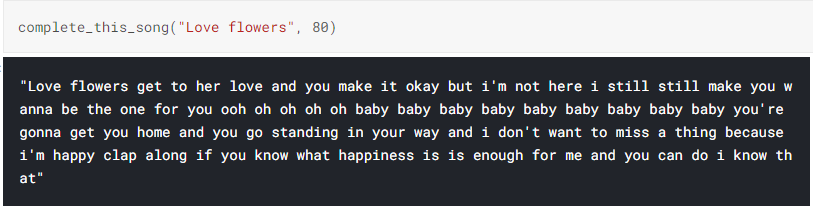
\includegraphics[width=13cm]{./imagenes/Analisis/Lstm1.png}
	   		\centering 
	   		\caption{Texto generado utilizando LSTM y la oración en inglés "Love flowers"}
	   	\end{figure}
   	
	   	\begin{figure}[H]
	   		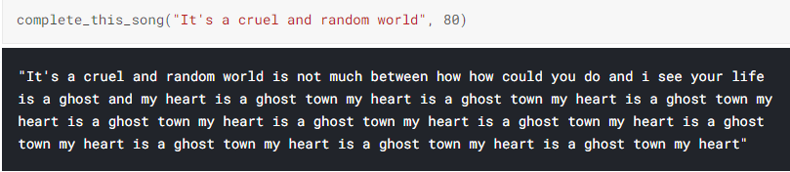
\includegraphics[width=13cm]{./imagenes/Analisis/Lstm2.png}
	   		\centering 
	   		\caption{Texto generado utilizando LSTM y la oración en inglés "It's a cruel and random world"}
	   	\end{figure}
	   	
	   	\newpage
	   	
	   	\subsection{Pruebas con BERT}
	   	Como última prueba fue generar algunos textos utilizando BERT, pero desafortunadamente estas pruebas no fueron exitosas debido a que si se desea trabajar con este algoritmo se requiere hacer uso de Tensorflow y para trabajar con esta biblioteca es necesario contar con una tarjeta de video de Nvidia con características específicas como los son la capacidad de la memoria de dicha tarjeta, hardware con el que no contamos. Se intentaron realizar las pruebas, pero se obtuvo lo siguiente: 
	   	\begin{figure}[H]
	   		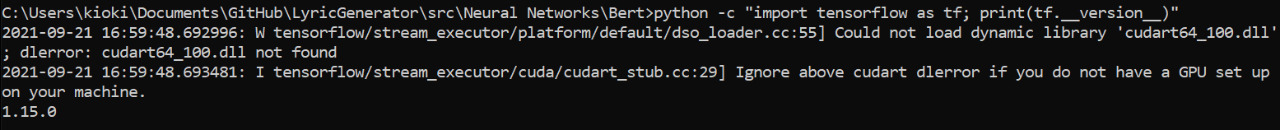
\includegraphics[width=13.5cm]{./imagenes/Analisis/ErrorBert.png}
	   		\centering 
	   		\caption{Error tensorflow BERT}
	   	\end{figure}
	   	En la imagen anterior se observa que tensorflow requiere del archivo cudart64\_100.dll disponible solo en tarjetas de video de Nvidia y siendo más específicos en las llamadas  CUDA GPUs las cuales son aquellas tarjetas de video de la familia RTX o Quadro y que para trabajar con CUDA (Arquitectura Unificada de Dispositivos de Cómputo) requiere de un gran ancho de banda en la memoria de las tarjetas y los dispositivos de la familias antes mencionadas son los que cuentan con la arquitectura y la capacidad de memoria para realizar estas tareas.
	   	

    	\section{Estudio de factibilidad}
    	El estudio de factibilidad es un instrumento que sirve para orientar la toma de decisiones, así como para determinar la posibilidad de desarrollar un negocio o proyecto; corresponde a la última fase de la etapa pre-operativa del ciclo del proyecto. Se formula con base en información que tiene la menor incertidumbre posible para medir las posibilidades de éxito o fracaso de un proyecto, apoyándose en el resultado se tomará la decisión de proceder o no con su implementación.\\\\ 
    	Este estudio establecerá la viabilidad, si existe, del trabajo planteado previamente.
    	\begin{itemize}
    		\item \textbf{Factibilidad Técnica:} Este aspecto evalúa que la infraestructura, es decir, equipos, software, conocimiento, experiencia, etc. que se poseen son los necesarios para efectuar las actividades requeridas para la realización del trabajo terminal.
    		\item \textbf{Factibilidad Operativa:} Analiza si el personal posee las competencias necesarias para el desarrollo del proyecto.
    		\item \textbf{Factibilidad Económica:} Consiste en el análisis de los recursos financieros necesarios para llevar a cabo la elaboración de este proyecto.
    	\end{itemize}
    	\subsection{Factibilidad técnica}
    	
    	Dentro de este apartado se explican detalladamente las tecnologías que se utilizarán, así como las características de nuestros equipos de cómputo actualmente. La elección de estas herramientas estuvo basada tanto en las tecnologías que más se utilizan en la actualidad como las que cuentan con el mayor soporte para su trabajo en la nube, esto se debe a que los equipos actuales no soportarían todo el trabajo.
    	    	
    	\begin{table}[H]
    		\caption[Equipo de cómputo ideal]{Equipo de cómputo ideal}
    		\begin{tabular}{|p{3.5cm}||p{10cm}|}
    			\rowcolor{guindapoli}
    			\multicolumn{2}{|c|}{\textbf{\textcolor{white}{Equipo de cómputo ideal.}}}\\
    			\hline
    			\rowcolor{azulclaro}Procesador & Intel i9 10900KF\\
    			\hline
    			\rowcolor{white}Tarjeta de video & NVIDIA RTX 3080 10Gb\\
    			\hline
    			\rowcolor{azulclaro}Memoria RAM & 32Gb DDR4\\
    			\hline
    			\rowcolor{white}Disco duro & 2Tb HDD y 512Gb SSD\\
    			\hline
    		\end{tabular}
    	\end{table}
    	
    	En la tabla anterior se muestra el equipo que requeriríamos para poder trabajar sin mayor dificultad al momento de realizar los entrenamientos de los modelos de redes neuronales que necesitamos para la realización de este trabajo, debido a la situación actual de alzas en precios muy altas, en el mercado actual los componentes para el equipo son escasos y su precio en el mercado aumento. Por esa razón se utilizarán servicios de la nube para la realización de estos entrenamientos y nuestros equipos para el desarrollo del resto del proyecto.
    	
    	\begin{table}[H]
    		\caption[Herramientas de software a utilizar]{Herramientas de software a utilizar}
    		\begin{tabular}{ |p{3.5cm}|p{9.5cm}|}
    			\hline
    			\rowcolor{guindapoli}
    			\multicolumn{2}{|c|}{\textbf{\textcolor{white}{Herramientas de Software a utilizar}}}\\
    			\hline
    			\cellcolor{azulclaro}Sistema Operativo & 
    			Linux, Mac, Windows \\ 
    			\hline
    			\cellcolor{azulclaro}Navegador Web &
    			Google Chrome\\
    			\hline
    			\cellcolor{azulclaro}Lenguaje de Programación &
    			Python\\
    			\hline
    			\cellcolor{azulclaro}Servidor &
    			Apache y Gunicorn\\
    			\hline
    			\cellcolor{azulclaro}Servicio Nube &
    			Amazon Web Services\\
    			\hline    			
    		\end{tabular}
    	\end{table}
    
    	Además de las herramientas de software a utilizar, es necesario mencionar el equipo de hardware que se utiliza, tanto para desarrollar, como para probar e implementar cada uno de los prototipos a lo largo de este trabajo terminal.
    	
        \begin{table}[H]
        	\caption[Equipo de cómputo 1]{Equipo de cómputo 1}
	    	\begin{tabular}{|p{3.5cm}||p{10cm}|}
	    		\rowcolor{guindapoli}
	    		\multicolumn{2}{|c|}{\textbf{\textcolor{white}{Equipo de cómputo 1 utilizado.}}}\\
	    		\hline
	    		\rowcolor{azulclaro}Procesador & Ryzen 5 3600\\
	    		\hline
	    		\rowcolor{white}Tarjeta de video & Amd Radeon Rx580\\
	    		\hline
	    		\rowcolor{azulclaro}Memoria RAM & 32 Gb\\
	    		\hline
	    		\rowcolor{white}Disco duro & 1Tb \acrshort{hdd} y 512Gb \acrshort{ssd}\\
	    		\hline
	    	\end{tabular}
   	  \end{table}
      \begin{table}[H]
      	\caption[Equipo de cómputo 2]{Equipo de cómputo 2}
	    	\begin{tabular}{|p{3.5cm}||p{10cm}|}
	    		\rowcolor{guindapoli}
	    		\multicolumn{2}{|c|}{\textbf{\textcolor{white}{Equipo de cómputo 2 utilizado.}}}\\
	    		\hline
	    		\rowcolor{azulclaro}Marca & Apple\\
	    		\hline
	    		\rowcolor{white}Modelo & iMac Late 2012\\
	    		\hline
	    		\rowcolor{azulclaro}Procesador & Intel Core i5\\
	    		\hline
	    		\rowcolor{white}Tarjeta de video & NVIDIA GeForce GT 640M 512 Mb\\
	    		\hline
	    		\rowcolor{azulclaro}Memoria RAM & 8 Gb\\
	    		\hline
	    		\rowcolor{white}Disco duro & 1Tb y 256 Gb \acrshort{ssd}\\
	    		\hline
	    	\end{tabular}
    \end{table}
    \begin{table}[H]
    	\caption[Equipo de cómputo 3]{Equipo de cómputo 3}
			\begin{tabular}{|p{3.5cm}||p{10cm}|}
				\rowcolor{guindapoli}
				\multicolumn{2}{|c|}{\textbf{\textcolor{white}{Equipo de cómputo 3 utilizado.}}}\\
				\hline
				\rowcolor{azulclaro}Procesador & Amd FX-8350\\
				\hline
				\rowcolor{white}Tarjeta de video & Nvidia Geforce 1050ti\\
				\hline
				\rowcolor{azulclaro}Memoria RAM & 16 Gb\\
				\hline
				\rowcolor{white}Disco duro & 1Tb \acrshort{hdd}\\
				\hline
			\end{tabular}
   \end{table}
\newpage
    	Junto con las herramientas de hardware y software a utilizar es necesario mencionar los servicios básicos que son relevantes para el desarrollo de este trabajo terminal como lo son:
    	\begin{itemize}
    		\item Luz Eléctrica
    		\item Agua Potable
    		\item Internet
    	\end{itemize}
    	Estos servicios forman parte de la factibilidad técnica ya que sin ellos no se podría realizar este proyecto y por eso mismo generan un costo, este mismo se desglosa más adelante en la sección \ref{FactibilidadEconomica}.
    	
    	\subsection{Factibilidad operativa}
    	A continuación se presenta una tabla con los recursos operativos del trabajo terminal que se calcularon con base en los recursos humanos con los que se cuenta actualmente y un análisis de las horas en las que el personal estará en operación:
    	
    	\begin{table}[h!]
    		\caption[Horas de trabajo]{Relación de horas de trabajo estimadas para la realización de este trabajo terminal}
    		\begin{tabular}{|p{2cm}|p{1.4cm}|p{2.2cm}|p{1.6cm}|p{2.2cm}|p{1.6cm}|}
    			\hline    			
    			\rowcolor{guindapoli}
    			\multicolumn{6}{|c|}{\textbf{\textcolor{white}{Horas a trabajar en el desarrollo del trabajo terminal}}}\\
    			\hline
    			Mes & No. de Días & Sábado y Domingo & Días hábiles & Horas de trabajo por día & Horas Totales \\
    			\hline
    			Marzo & 31 & 8 & 22 & 2 & 44 \\ 
    			\hline
    			Abril & 30 & 8 & 15 & 2 & 30 \\ 
    			\hline
    			Mayo & 31 & 10 & 19 & 2 & 38 \\
    			\hline
    			Junio & 30 & 10 & 17 & 2 & 34 \\
    			\hline
    			Agosto & 31 & 10 & 18 & 2 & 24 \\
    			\hline
    			Septiembre & 30 & 8 & 20 & 2 & 40 \\ 
    			\hline
    			Octubre & 31 & 10 & 20 & 2 & 40 \\ 
    			\hline
    			Noviembre & 31 & 8 & 18 & 2 & 36 \\ 
    			\hline
    		\end{tabular}
    	\end{table}
    	Con esto podemos concluir que contamos con 286 horas, suficiente tiempo para el desarrollo de este trabajo terminal, ya que las horas totales de trabajo están contempladas para cada uno de los integrantes del equipo
    	
    	\subsection{Factibilidad económica\label{FactibilidadEconomica}}
    	Luego de haber realizado el estudio de factibilidad técnica así como el operacional es necesario tomar en cuenta un estudio de factibilidad económica el cual desglosará todo el gasto económico realizado para la elaboración de este trabajo terminal:
    	\begin{itemize}
    		\item \textbf{Capital Humano:} Se tienen contemplados aproximadamente 36 días laborales, es decir, 288 horas para la elaboración de este trabajo terminal en el cual participaremos los tres integrantes
    		\item \textbf{Capital Técnico:} Se cuenta con las viviendas y el equipo de cómputo principal de cada uno de los integrantes.
    	\end{itemize}
    	Respecto a los costos monetarios de todo el proyecto se toma a consideración lo siguiente:
    	\begin{itemize}
    		\item \textbf{Servicios}\\
    		Se considera un gasto mensual aproximado de \$1,400.00 que al ser multiplicado por todo el tiempo de elaboración contemplado nos da un total de \$11,200.00, por integrante.
    		\item \textbf{Software} \\
    		Durante algunos periodos se va a hacer uso principalmente de herramientas gratuitas y de software libre, en cuanto al servicio en la nube se pretende hacer uso de \acrshort{aws} y trabajar inicialmente con los planes gratuitos que ofrece, en caso de que se lleguen a consumir los recursos de este plan, entonces se procederá a hacer el cambio a otro plan superior donde el costo actual se cobra en \$ 0.15 centavos de dólar por hora de uso.
    		\item \textbf{Hardware}\\
    		Se utilizarán los equipos de cómputo personal de cada integrante, lo que da un costo aproximado de \$24,012.00 aplicando los parámetros de vida útil de un equipo de cómputo y su depreciación anual del hardware. 
    		\item \textbf{Recursos Humanos}\\
    		Se estima un gasto aproximado de \$12,000.00 por cada integrante del equipo para la elaboración del proyecto con lo que se generará un gasto total de \$36,000.00
    	\end{itemize}
    	Tomando en cuenta el salario promedio de un desarrollador de software el cual es de \$15,000.00 mensuales, dato fundamentado en la búsqueda de salario promedio en la página web de mx.indeed.com, se consideró este salario para el desarrollo del proyecto, el cual tendría una duración de 8 meses aproximadamente para finalizar este proyecto, dando como resultado un salario total para los integrantes del equipo de \$360,000.00; el costo final del desarrollo de este trabajo terminal sería de: \\
    	\begin{center}
    		\$453,612.00
    	\end{center}
    	\textbf{Conclusión\\} 
    	Tras realizar el estudio de factibilidad en este proyecto, es pertinente decir que los integrantes no cuentan con el apoyo financiero y que el hardware mencionado ya es propiedad de los integrantes, por lo que el trabajo terminal se califica como \textit{“Viable”} iniciando de manera inmediata su implementación acorde las fechas mencionadas.
    	
    	\subsection{Aspectos económicos}
    	Las herramientas que usaremos en el trabajo terminal y las cuales validarán la viabilidad del proyecto se presentan a continuación:\\\\
    	Herramientas Open Source a utilizar en el presente trabajo terminal
    	
    	\begin{itemize}
    		\item Datamuse API \cite{refDatamuseLicense}
    		\item MongoDB - SSPL* \cite{refMongoDBLicense}
    		\item \acrshort{bert} - Apache 2.0 \cite{refBERTLicense}
    		\item Apache - Apache 2.0 \cite{refApacheLicense}
    		\item React - MIT \cite{refReactLicense}
    		\item Python - PSFL \cite{refPythonLicense}
    		\item Amazon - Elastic 2.0 y SSPL \cite{refAmazonLicense}
    	\end{itemize}
    	
    	*SSPL: Aunque es clasificado como Open Source por parte de MongoDB, al estar basado en la licencia de software libre de GPL3, la Iniciativa de Open Source (OSI) no la reconoce como licencia Open Source al describirla como una “licencia Open Source no genuina".\\
    	
    	Como se puede apreciar en el software presentado, las licencias son del tipo Open Source con lo cual validamos la viabilidad económica del proyecto el cual no representará gasto monetario más allá del necesitado para el entrenamiento de la red neuronal, para el cual haremos uso de Amazon SageMaker que tiene un costo de:\\\\
    	Cuota gratuita primeros 2 meses:
    	\begin{itemize}
    		\item Instancia de bloc de notas: 250 horas.
    		\item Entrenamiento: 50 horas. 
    	\end{itemize}
    	Cuotas:
    	\begin{itemize}
    		\item Instancia de bloc de notas (4 CPU's virtuales y 16Gb de memoria): 0.20 centavos de dólar/hora.
    		\item Entrenamiento (4 CPU's virtuales y 16Gb de memoria): 0.23 centavos de dólar/hora.
    		\item Procesamiento (4 CPU's virtuales y 16Gb de memoria): 0.20 centavos de dólar/hora.
    	\end{itemize}	
    	
    	% Aquí van las licencias, descripción, software a utilizar, precio
    	\subsection{Aspectos legales}
    	\subsubsection*{Copyright}
    	Los derechos de autor son una forma de protección para obras originales de autoría fijadas en un medio de expresión tangible. Los derechos de autor cubren tanto las obras publicadas como las que no o son inéditas.\cite{refCopyright}\\\\
    	Los derechos de autor protegen un gran rango de obras como lo son: obras literarias, musicales, pictóricas o escultóricas, coreografías, escenas dramáticas, producciones cinematográficas y demás audiovisuales, programas de cómputo, fotografías, entre muchas otras.
    	\subsubsection*{Originalidad}
    	Los derechos de autor protegen la forma en que se expresan las ideas. Esta manera única de expresar las palabras, notas musicales, colores, formas, etc. son elegidas y organizadas u ordenadas. Es la expresión lo que hace que una obra sea original. Esto significa que puede haber muchos trabajos diferentes sobre la misma idea y todos de ellos estarán protegidos por derechos de autor, siempre y cuando expresen esta idea de una manera original.\cite{refOriginalidadWipo}\\\\
    	Según la Ley Federal del Derecho de Autor, la forma en cómo se expresa un autor al momento de crear su obra es lo que esta protegido por la ley ante acciones fraudulentas.\cite{refOriginalidadLFDA}\\\\
    	Con base en la Ley Federal del Derecho de Autor Capitulo IV articulo 107 “Las bases de datos o de otros materiales legibles por medio de máquinas o en otra forma, que por razones de selección y disposición de su contenido constituyan creaciones intelectuales, quedarán protegidas como compilaciones."\cite{refOriginalidadLFDA}\\\\
    	Por ende las canciones generadas por nuestro sistema no se pretenden ni pueden registrar, ya que estos resultados generados serian nuestros.
    	
    	\section{Análisis de riesgo}
    	Dentro de este apartado determinaremos la probabilidad de que surja alguna problemática o riesgo el cual pueda impactar el desarrollo del proyecto, ya sea en términos del cronograma, la calidad o los costos.\\\\
    	Algunos riesgos que enfrentaremos durante el desarrollo del proyecto son los siguientes:\par
    	\begin{itemize}
    		\item \textbf{Riesgo de costo}\\
	    	Si sobrepasamos el costo de desarrollo previsto, quizá nos enfrentemos a problemas relacionados con el alcance y los requerimientos tanto funcionales como los que no lo son del proyecto.
	    	\begin{table}[hbt!]\caption{Riesgo de costo}% title of Table
	    		\centering % used for centering table
	    		\resizebox{8cm}{!} {
	    			\begin{tabular}{|c|c|}% centered columns (3 columns)
	    				\hline                        %inserts double horizontal lines
	    				\multicolumn{2}{|c|}{Riesgo: Costos Elevados}\\% inserts table %heading
	    				\hline                  % inserts single horizontal line
	    				\begin{tabular}[c]{@{}l@{}}Impacto: Medio alto (7).\end{tabular}
	    				& \begin{tabular}[c]{@{}l@{}}Nivel: Alto (49)\end{tabular} \\% inserting body of the table 
	    				\hline
	    				\begin{tabular}[c]{@{}l}Probabilidad: Medio alto (7)\end{tabular}
	    				& \begin{tabular}[c]{@{}l@{}}\end{tabular} \\
	    				\hline
	    			\end{tabular}\label{table:Riesgo de Costo}% is used to refer this table in the text
	    		}
	    	\end{table}
    	
    		\begin{figure}[H]
    			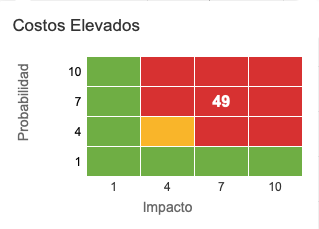
\includegraphics[width=9cm]{./imagenes/Analisis/AnalisisRiesgo/Costos_elevados.png}
    			\centering 
    			\caption{Matriz de riesgo de costo}
    		\end{figure}
	    	
	    	\item \textbf{Riesgo de calendario}\\
	    	Si se realizó una mala estimación del tiempo necesario para el desarrollo, se asignaron mal los recursos o si hubo alguna afectación dentro del recurso humano, lo más probable es que el proyecto no se termine de desarrollar en el tiempo establecido.
	    	
	    	\begin{table}[hbt!]\caption{Riesgo de calendario}% title of Table
	    		\centering % used for centering table
	    		\resizebox{8cm}{!} {
	    			\begin{tabular}{|c|c|}% centered columns (3 columns)
	    				\hline                        %inserts double horizontal lines
	    				\multicolumn{2}{|c|}{Riesgo: Falta de Tiempo}\\% inserts table %heading
	    				\hline                  % inserts single horizontal line
	    				\begin{tabular}[c]{@{}l@{}}Impacto: Medio bajo (4).\end{tabular}
	    				& \begin{tabular}[c]{@{}l@{}}Nivel: Medio Medio (16)\end{tabular} \\% inserting body of the table 
	    				\hline
	    				\begin{tabular}[c]{@{}l}Probabilidad: Medio bajo (4)\end{tabular}
	    				& \begin{tabular}[c]{@{}l@{}}\end{tabular} \\
	    				\hline
	    			\end{tabular}\label{table:Riesgo de calendario}% is used to refer this table in the text
	    		}
	    	\end{table}
	    	
	    	\begin{figure}[H]
	    		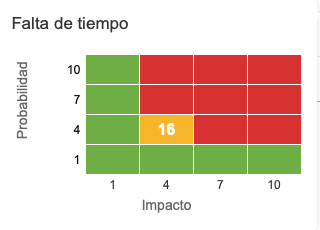
\includegraphics[width=9cm]{./imagenes/Analisis/AnalisisRiesgo/faltadetiempo.png}
	    		\centering 
	    		\caption{Matriz de riesgo de calendario}
	    	\end{figure}
	    	
	    	\item \textbf{Riesgo tecnológico}\\
	    	Si no logramos entender la complejidad de las herramientas que utilizaremos para el desarrollo del proyecto o nos toma demasiado tiempo que son nuevas para nosotros, como lo son la herramientas de AWS para la creación de los modelos de redes neuronales y su entrenamiento dentro de la misma plataforma, se podrían presentar problemas como: integración a la página web, creación fallida de los modelos de las redes neuronales, falta de adaptación con el hardware utilizado, entre otros.
	    	
	    	\begin{table}[hbt!]\caption{Riesgo tecnológico}% title of Table
	    		\centering % used for centering table
	    		\resizebox{8cm}{!} {
	    			\begin{tabular}{|c|c|}% centered columns (3 columns)
	    				\hline                        %inserts double horizontal lines
	    				\multicolumn{2}{|c|}{Riesgo: Fallas de Equipos}\\% inserts table %heading
	    				\hline                  % inserts single horizontal line
	    				\begin{tabular}[c]{@{}l@{}}Impacto: Bajo (1).\end{tabular}
	    				& \begin{tabular}[c]{@{}l@{}}Nivel: Bajo (7)\end{tabular} \\% inserting body of the table 
	    				\hline
	    				\begin{tabular}[c]{@{}l}Probabilidad: Medio alto (7)\end{tabular}
	    				& \begin{tabular}[c]{@{}l@{}}\end{tabular} \\
	    				\hline
	    			\end{tabular}\label{table:Riesgo_tecnologico}% is used to refer this table in the text
	    		}
	    	\end{table}
	    	
	    	\begin{figure}[H]
	    		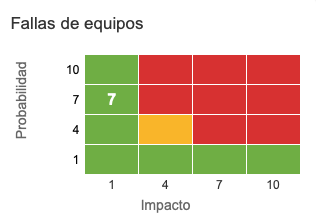
\includegraphics[width=9cm]{./imagenes/Analisis/AnalisisRiesgo/Fallas_equipo.png}
	    		\centering 
	    		\caption{Matriz de riesgo tecnológico}
	    	\end{figure}
	    	
	    	\item \textbf{Riesgo operacional}\\
	    	Si no se plantean posibles soluciones a problemas que podrían suceder durante el proyecto, si no se presenta un correcto liderazgo y buenas aportaciones por parte de uno o más miembros, si existe una mala comunicación, falta de motivación y si no hay una monitorización, se puede ver mermado el avance del proyecto.
	    	
	    	\begin{table}[hbt!]\caption{Riesgo operacional}% title of Table
	    		\centering % used for centering table
	    		\resizebox{8cm}{!} {
	    			\begin{tabular}{|c|c|}% centered columns (3 columns)
	    				\hline                        %inserts double horizontal lines
	    				\multicolumn{2}{|c|}{Riesgo: Desorganización en el equipo}\\% inserts table %heading
	    				\hline                  % inserts single horizontal line
	    				\begin{tabular}[c]{@{}l@{}}Impacto: Medio bajo (4).\end{tabular}
	    				& \begin{tabular}[c]{@{}l@{}}Nivel: Medio (16)\end{tabular} \\% inserting body of the table 
	    				\hline
	    				\begin{tabular}[c]{@{}l}Probabilidad: Medio bajo (4)\end{tabular}
	    				& \begin{tabular}[c]{@{}l@{}}\end{tabular} \\
	    				\hline
	    			\end{tabular}\label{table:Riesgo_operacional}% is used to refer this table in the text
	    		}
	    	\end{table}
	    	
	    	\begin{figure}[H]
	    		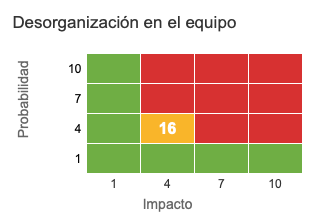
\includegraphics[width=9cm]{./imagenes/Analisis/AnalisisRiesgo/Desorganizacion.png}
	    		\centering 
	    		\caption{Matriz de riesgo operacional}
	    	\end{figure}
	    	
	    	\item \textbf{Riesgos externos}\\
	    	Factores fuera de nuestro alcance que pueden afectar el desarrollo del proyecto, entre ellos puede ser algún cambio en las leyes, en alguna norma, desastre natural, etc.
	    	
	    	\begin{table}[hbt!]\caption{Riesgos externos}% title of Table
	    		\centering % used for centering table
	    		\resizebox{8cm}{!} {
	    			\begin{tabular}{|c|c|}% centered columns (3 columns)
	    				\hline                        %inserts double horizontal lines
	    				\multicolumn{2}{|c|}{Riesgo: Factores Externos}\\% inserts table %heading
	    				\hline                  % inserts single horizontal line
	    				\begin{tabular}[c]{@{}l@{}}Impacto: Alto (10).\end{tabular}
	    				& \begin{tabular}[c]{@{}l@{}}Nivel: Bajo (10)\end{tabular} \\% inserting body of the table 
	    				\hline
	    				\begin{tabular}[c]{@{}l}Probabilidad: Bajo (1)\end{tabular}
	    				& \begin{tabular}[c]{@{}l@{}}\end{tabular} \\
	    				\hline
	    			\end{tabular}\label{table:Riesgos externos}% is used to refer this table in the text
	    		}
	    	\end{table}
	    	
	    	\begin{figure}[H]
	    		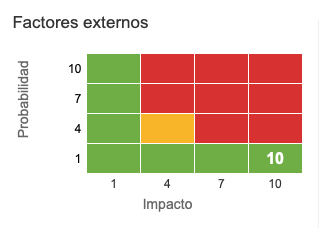
\includegraphics[width=9cm]{./imagenes/Analisis/AnalisisRiesgo/Externos.png}
	    		\centering 
	    		\caption{Matriz de riesgos externos}
	    	\end{figure}
	    	
    	\end{itemize}
    
    	\begin{figure}[H]
    		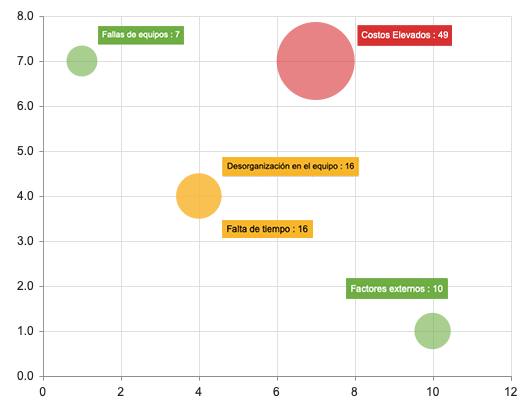
\includegraphics[width=9cm]{./imagenes/Analisis/AnalisisRiesgo/analisisriesgos.png}
    		\centering 
    		\caption{Matriz general de riesgos}
    	\end{figure}
    
    	Se utilizó la herramienta llamada ``Matriz de Evaluación de Riesgos de ITM Platform'' para generar este análisis de riesgo. \cite{refMatrizEvaluacionRiesgos}
\newpage

\chapter{\textcolor{azulescom}{Diseño}}

%%%%%%%%%%%%%%%%%%%%%%%%%%%%%%%%%%%%%%%%%%%%%%%%%%%%%%%%%
%                                                       																																		  %
%                                                      																																	  		  %
%              													 Arquitectura de Sistema  																				   %
%                                                      																																			  %
%                                                      																																			  %
%%%%%%%%%%%%%%%%%%%%%%%%%%%%%%%%%%%%%%%%%%%%%%%%%%%%%%%%%
\section{Arquitectura del sistema}
		\subsection{Descripción de la arquitectura del sistema}
		Para poder crear esta herramienta de apoyo para estudiantes o aficionados en el área musical con la creación de letras musicales, se propone crear un sistema basado en inteligencia artificial usando técnicas de procesamiento de lenguaje natural que pueda auxiliarlos y puedan lograr su meta propuesta.\\\\	
		El sistema se compone de tres bloques los cuales se comunicarán vía red:
		\begin{enumerate}
			\item \textbf{Base de datos:} En este módulo se almacenan los datos de canciones, se trabajará especialmente con una tabla que contenga como principales campos:
			\begin{itemize}
				\item Artista
				\item Género
				\item Nombre de la Canción
				\item Letra
				\item Idioma
			\end{itemize}
			Dicha base de datos se almacenará en un sistema especializado que se conecte a la nube para poder trabajar y almacenar estos datos sin mayor problema.
			\item \textbf{Modelado de la red neuronal:} Este bloque va ser el encargado de generar las letras musicales para cada usuario que ingrese. Para la generación de dichas letras musicales, se utilizará un servicio en la nube para procesar la solicitud del usuario. 
			\item \textbf{Página Web}: Este primer bloque es el que se encuentra directamente enlazado con el usuario de nuestro sistema y al mismo tiempo con el servicio en la nube que aloja a las redes neuronales, el usuario utilizando su navegador podrá realizar peticiones al servicio en la web.
		\end{enumerate}
	
		\subsection{Funcionamiento general del sistema}
		El siguiente diagrama muestra como se espera que quede el funcionamiento general del proyecto.
	
		\begin{figure}[H] 
			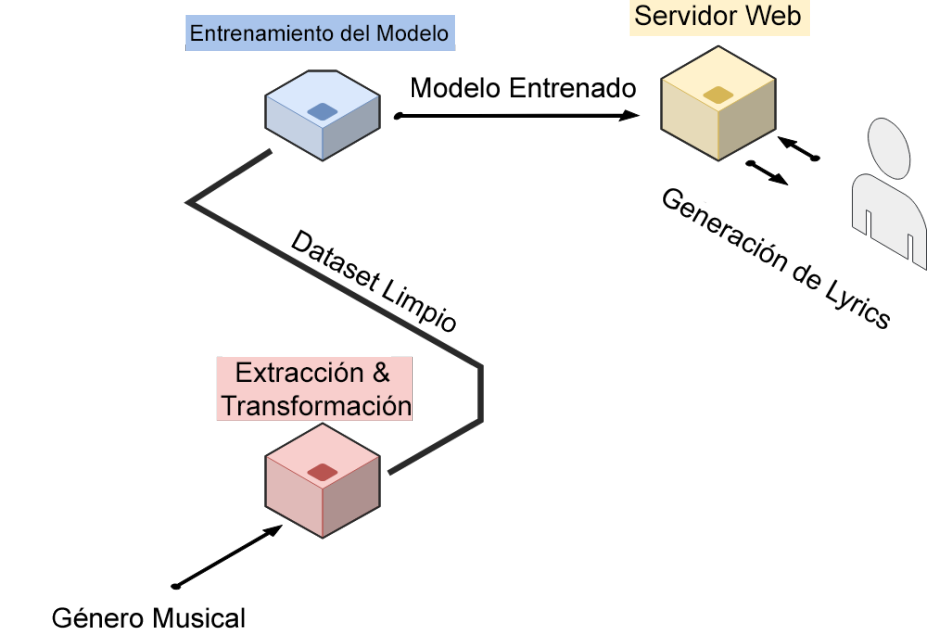
\includegraphics[scale=.4]{./imagenes/Disenio/Arquitectura/general.png}
			\caption{Diagrama general del sistema}
		\end{figure}
		Como se observa en la figura anterior, se tendrán tres procesos principales para lograr el objetivo final.\\\\
		En primer instancia se tendrá que obtener la base de datos y por medio de extracción y transformación, se obtendrá el dataset deseado para poder generar el modelo. \\\\
		Después de un proceso de limpieza de este dataset, se hará un entrenamiento del modelo en la nube para poder generar funciones utilizando este modelo para poder generar textos.
		una vez teniendo esta aplicación funcional, se configurará el servidor web para que se pueda comunicar con el usuario final y con la aplicación que utiliza el modelo vía web, logrando así los objetivos.
	
		\subsection{Diagrama caso de uso}
		
		A continuación mostramos el caso de uso de nuestra aplicación web y su interacción con el usuario:
		
		\begin{figure}[H] 
			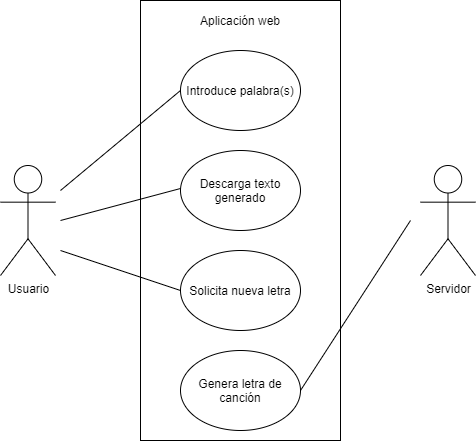
\includegraphics[scale=.75]{./imagenes/Disenio/Arquitectura/CasoUso.png}
			\centering 
			\caption{Diagrama de caso de uso}
		\end{figure}
		\newpage
		\begin{table}[hbt!]\caption{Caso de uso 1}% title of Table
			\centering % used for centering table
			\resizebox{13.5cm}{!} {
				\begin{tabular}{|c|c|}% centered columns (3 columns)
					\hline                        %inserts double horizontal lines
					\begin{tabular}[c]{@{}l@{}}Caso de uso\end{tabular}
					& \begin{tabular}[c]{@{}l@{}}Introduce palabra en inglés\end{tabular} \\% inserting body of the table 
					\hline				                     
					\begin{tabular}[c]{@{}l@{}}Actores\end{tabular}
					& \begin{tabular}[c]{@{}l@{}}Usuario\end{tabular} \\% inserting body of the table 
					\hline
					\begin{tabular}[c]{@{}l@{}}Descripción\end{tabular}
					& \begin{tabular}[c]{@{}l@{}}El usuario dentro de la aplicación web proporciona una palabra\\ en el idioma inglés para con ella poder generar un texto \end{tabular} \\
					\hline
				\end{tabular}\label{table:Caso de uso 1}% is used to refer this table in the text
			}
		\end{table}
		\begin{table}[hbt!]\caption{Caso de uso 2}% title of Table
			\centering % used for centering table
			\resizebox{13.5cm}{!} {
				\begin{tabular}{|c|c|}% centered columns (3 columns)
					\hline                        %inserts double horizontal lines
					\begin{tabular}[c]{@{}l@{}}Caso de uso\end{tabular}
					& \begin{tabular}[c]{@{}l@{}}Descargar texto generado\end{tabular} \\% inserting body of the table 
					\hline				                     
					\begin{tabular}[c]{@{}l@{}}Actores\end{tabular}
					& \begin{tabular}[c]{@{}l@{}}Usuario\end{tabular} \\% inserting body of the table 
					\hline
					\begin{tabular}[c]{@{}l@{}}Descripción\end{tabular}
					& \begin{tabular}[c]{@{}l@{}}El usuario dentro de la aplicación web tiene la posibilidad\\ de descargar el texto generado por el modelo  \end{tabular} \\
					\hline
				\end{tabular}\label{table:Caso de uso 2}% is used to refer this table in the text
			}
		\end{table}	
		\begin{table}[hbt!]\caption{Caso de uso 3}% title of Table
			\centering % used for centering table
			\resizebox{13.5cm}{!} {
				\begin{tabular}{|c|c|}% centered columns (3 columns)
					\hline                        %inserts double horizontal lines
					\begin{tabular}[c]{@{}l@{}}Caso de uso\end{tabular}
					& \begin{tabular}[c]{@{}l@{}}Solicitar nueva letra\end{tabular} \\% inserting body of the table 
					\hline				                     
					\begin{tabular}[c]{@{}l@{}}Actores\end{tabular}
					& \begin{tabular}[c]{@{}l@{}}Usuario\end{tabular} \\% inserting body of the table 
					\hline
					\begin{tabular}[c]{@{}l@{}}Descripción\end{tabular}
					& \begin{tabular}[c]{@{}l@{}}Al usuario dentro de la aplicación web se le da posibilidad de volver\\ a generar otra letra musical usando los mismos parámetros que proporcionó\\ o utilizando unos nuevos\end{tabular} \\
					\hline
				\end{tabular}\label{table:Caso de uso 3}% is used to refer this table in the text
			}
		\end{table}	
		\begin{table}[hbt!]\caption{Caso de uso 4}% title of Table
			\centering % used for centering table
			\resizebox{13.5cm}{!} {
				\begin{tabular}{|c|c|}% centered columns (3 columns)
					\hline                        %inserts double horizontal lines
					\begin{tabular}[c]{@{}l@{}}Caso de uso\end{tabular}
					& \begin{tabular}[c]{@{}l@{}}Genera letra de canción\end{tabular} \\% inserting body of the table 
					\hline				                     
					\begin{tabular}[c]{@{}l@{}}Actores\end{tabular}
					& \begin{tabular}[c]{@{}l@{}}Servidor\end{tabular} \\% inserting body of the table 
					\hline
					\begin{tabular}[c]{@{}l@{}}Descripción\end{tabular}
					& \begin{tabular}[c]{@{}l@{}}El servidor envia el texto generado por el modelo a la aplicación web,\\ la cual se encarga de mostrarla al usuario final \end{tabular} \\
					\hline
				\end{tabular}\label{table:Caso de uso41}% is used to refer this table in the text
			}
		\end{table}
		\newpage
		\subsection{Historias de usuario}
		
		\begin{table}[hbt!]\caption{Historia de usuario 1}% title of Table
			\centering % used for centering table
			\resizebox{15cm}{!} {
				\begin{tabular}{|c|c|}% centered columns (3 columns)
					\hline                        %inserts double horizontal lines
					\multicolumn{2}{|c|}{Historia de usuario 1}\\% inserts table %heading
					\hline                  % inserts single horizontal line
					 \begin{tabular}[c]{@{}l@{}}Nombre: Generar una letra de canción.\end{tabular}
					& \begin{tabular}[c]{@{}l@{}}Usuario: Visitante\end{tabular} \\% inserting body of the table 
					\hline
					\begin{tabular}[c]{@{}l@{}}Descripción: Como un visitante de la\\ página web quiero generar una\\ letra de una canción a partir de una palabra\\ que proporcione.\end{tabular}
					& \begin{tabular}[c]{@{}l@{}}Validación: Con la palabra proporcionada\\ por el usuario y con ayuda del modelo\\ entrenado se generará una letra musical\\ relacionada a esta.\end{tabular} \\
					\hline
				\end{tabular}\label{table:Historia de usuario 1}% is used to refer this table in the text
			}
		\end{table}
	
		\begin{table}[hbt!]\caption{Historia de usuario 2}% title of Table
			\centering % used for centering table
			\resizebox{15cm}{!} {
				\begin{tabular}{|c|c|}% centered columns (3 columns)
					\hline                        %inserts double horizontal lines
					\multicolumn{2}{|c|}{Historia de usuario 2}\\% inserts table %heading
					\hline                  % inserts single horizontal line
					\begin{tabular}[c]{@{}l@{}}Nombre: Descargar una letra canción.\end{tabular}
					& \begin{tabular}[c]{@{}l@{}}Usuario: Visitante\end{tabular} \\% inserting body of the table 
					\hline
					\begin{tabular}[c]{@{}l@{}}Descripción: Como un visitante de la\\ página web quiero poder descargar\\ la letra de la canción que se generó\\ a partir de la palabra que proporcioné.\end{tabular}
					& \begin{tabular}[c]{@{}l@{}}Validación: El usuario podrá descargar\\ un archivo de texto que contendrá\\ la letra de la canción generada.\end{tabular} \\
					\hline
				\end{tabular}\label{table:Historia de usuario 2}% is used to refer this table in the text
			}
		\end{table}
	
		\begin{comment}		
		\begin{table}[hbt!]\caption{Historia de usuario 3}% title of Table
			\centering % used for centering table
			\resizebox{15cm}{!} {
				\begin{tabular}{|c|c|}% centered columns (3 columns)
					\hline                        %inserts double horizontal lines
					\multicolumn{2}{|c|}{Historia de usuario 3}\\% inserts table %heading
					\hline                  % inserts single horizontal line
					\begin{tabular}[c]{@{}l@{}}Nombre: Definir que tanto deseo que rime una canción\end{tabular}
					& \begin{tabular}[c]{@{}l@{}}Usuario: Visitante\end{tabular} \\% inserting body of the table 
					\hline
					\begin{tabular}[c]{@{}l@{}}Descripción: Me gustaría tener una opción\\ en la cual pueda definir que tanto quiero\\ rimar una canción, desde que\\ no rime nada hasta que rime toda. \end{tabular}
					& \begin{tabular}[c]{@{}l@{}}Validación: Se genera una letra de canción\\ con lo parámetros de rima que establece el\\ usuario.\end{tabular} \\
					\hline
				\end{tabular}\label{table:Historia de usuario 3}% is used to refer this table in the text
			}
		\end{table}			
		\end{comment}
	
		\begin{table}[hbt!]\caption{Historia de usuario 3}% title of Table
			\centering % used for centering table
			\resizebox{15cm}{!} {
				\begin{tabular}{|c|c|}% centered columns (3 columns)
					\hline                        %inserts double horizontal lines
					\multicolumn{2}{|c|}{Historia de usuario 3}\\% inserts table %heading
					\hline                  % inserts single horizontal line
					\begin{tabular}[c]{@{}l@{}}Nombre: Generar otra letra de canción con los mismos parámetros\end{tabular}
					& \begin{tabular}[c]{@{}l@{}}Usuario: Visitante\end{tabular} \\% inserting body of the table 
					\hline
					\begin{tabular}[c]{@{}l@{}}Descripción: Como usuario, me gustaría generar otra\\ letra de canción con los mismo parámetros y\\ palabra que ya había introducido.\end{tabular}
					& \begin{tabular}[c]{@{}l@{}}Validación: Brindar una opción al usuario\\ que una vez generada y desplegada la letra de\\ la canción pueda generar otra usando los\\ mismo parámetros que previamente había \\introducido.\end{tabular} \\
					\hline
				\end{tabular}\label{table:Historia de usuario 3}% is used to refer this table in the text
			}
		\end{table}
	
		\begin{table}[hbt!]\caption{Historia de usuario 4}% title of Table
			\centering % used for centering table
			\resizebox{15cm}{!} {
				\begin{tabular}{|c|c|}% centered columns (3 columns)
					\hline                        %inserts double horizontal lines
					\multicolumn{2}{|c|}{Historia de usuario 4}\\% inserts table %heading
					\hline                  % inserts single horizontal line
					\begin{tabular}[c]{@{}l@{}}Nombre: Validación de la palabra introducida.\end{tabular}
					& \begin{tabular}[c]{@{}l@{}}Usuario: Sistema\end{tabular} \\% inserting body of the table 
					\hline
					\begin{tabular}[c]{@{}l@{}}Descripción: La página web validará la palabra\\ proporcionada por el usuario para\\ con ella hacer la petición al servidor\\ y generar una letra de canción relacionada a esta. \end{tabular}
					& \begin{tabular}[c]{@{}l@{}}Validación: Con ayuda del modelo y la palabra\\ introducida y procesada por la página web\\ se genera y despliega la letra generada.\end{tabular} \\
					\hline
				\end{tabular}\label{table:Historia de usuario 4}% is used to refer this table in the text
			}
		\end{table}
		\begin{table}[hbt!]\caption{Historia de usuario 5}% title of Table
		\centering % used for centering table
		\resizebox{15cm}{!} {
			\begin{tabular}{|c|c|}% centered columns (3 columns)
				\hline                        %inserts double horizontal lines
				\multicolumn{2}{|c|}{Historia de usuario 5}\\% inserts table %heading
				\hline                  % inserts single horizontal line
				\begin{tabular}[c]{@{}l@{}}Nombre: Limpiar base de batos.\end{tabular}
				& \begin{tabular}[c]{@{}l@{}}Usuario: Desarrollador\end{tabular} \\% inserting body of the table 
				\hline
				\begin{tabular}[c]{@{}l@{}}Descripción: Como un desarrollador\\ quiero una base de datos\\sin caracteres especiales\\ o palabras repetidas.\end{tabular}
				& \begin{tabular}[c]{@{}l@{}}Validación: Con ayuda de un script\\ para quitar palabras innecesarias\\y caracteres inválidos\end{tabular} \\
				\hline
			\end{tabular}\label{table:Historia de usuario 5}% is used to refer this table in the text
		}
	\end{table}
		\begin{table}[hbt!]\caption{Historia de usuario 6}% title of Table
	\centering % used for centering table
	\resizebox{15cm}{!} {
		\begin{tabular}{|c|c|}% centered columns (3 columns)
			\hline                        %inserts double horizontal lines
			\multicolumn{2}{|c|}{Historia de usuario 6}\\% inserts table %heading
			\hline                  % inserts single horizontal line
			\begin{tabular}[c]{@{}l@{}}Nombre: Pre-procesar la base de datos.\end{tabular}
			& \begin{tabular}[c]{@{}l@{}}Usuario: Desarrollador\end{tabular} \\% inserting body of the table 
			\hline
			\begin{tabular}[c]{@{}l@{}}Descripción: Como un desarrollador\\ quiero generar el modelo\\solo con los datos necesarios\\ para optimizar los tiempos de entrenamiento.\end{tabular}
			& \begin{tabular}[c]{@{}l@{}}Validación: Con un script\\ para tokenizar y hacer pre-padding en\\ la base de datos\end{tabular} \\
			\hline
		\end{tabular}\label{table:Historia de usuario 6}% is used to refer this table in the text
	}
		\end{table}
				\begin{table}[hbt!]\caption{Historia de usuario 7}% title of Table
		\centering % used for centering table
		\resizebox{15cm}{!} {
			\begin{tabular}{|c|c|}% centered columns (3 columns)
				\hline                        %inserts double horizontal lines
				\multicolumn{2}{|c|}{Historia de usuario 7}\\% inserts table %heading
				\hline                  % inserts single horizontal line
				\begin{tabular}[c]{@{}l@{}}Nombre: Subir Base de Datos a la nube.\end{tabular}
				& \begin{tabular}[c]{@{}l@{}}Usuario: Desarrollador\end{tabular} \\% inserting body of the table 
				\hline
				\begin{tabular}[c]{@{}l@{}}Descripción: Como un desarrollador\\ quiero generar el modelo\\con los datos necesarios\\ en la nube para optimizar espacio local.\end{tabular}
				& \begin{tabular}[c]{@{}l@{}}Validación: Utilizando herramientas\\ NOSQL\\para subir la base de datos y esta no ocupe espacio local\end{tabular} \\
				\hline
			\end{tabular}\label{table:Historia de usuario 7}% is used to refer this table in the text
		}
	\end{table}
			\begin{table}[hbt!]\caption{Historia de usuario 8}% title of Table
		\centering % used for centering table
		\resizebox{15cm}{!} {
			\begin{tabular}{|c|c|}% centered columns (3 columns)
				\hline                        %inserts double horizontal lines
				\multicolumn{2}{|c|}{Historia de usuario 8}\\% inserts table %heading
				\hline                  % inserts single horizontal line
				\begin{tabular}[c]{@{}l@{}}Nombre: Generar Modelo en la nube.\end{tabular}
				& \begin{tabular}[c]{@{}l@{}}Usuario: Desarrollador\end{tabular} \\% inserting body of the table 
				\hline
				\begin{tabular}[c]{@{}l@{}}Descripción: Como un desarrollador\\ quiero generar nuevas letras de canciones\\a partir de un dataset proporcionado\\ anteriormente.\end{tabular}
				& \begin{tabular}[c]{@{}l@{}}Validación: Con un script en una plataforma en línea\\ entrenar el modelo para generar\\ nuevas canciones\end{tabular} \\
				\hline
			\end{tabular}\label{table:Historia de usuario 8}% is used to refer this table in the text
		}
	\end{table}
			\begin{table}[hbt!]\caption{Historia de usuario 9}% title of Table
	\centering % used for centering table
	\resizebox{15cm}{!} {
		\begin{tabular}{|c|c|}% centered columns (3 columns)
			\hline                        %inserts double horizontal lines
			\multicolumn{2}{|c|}{Historia de usuario 9}\\% inserts table %heading
			\hline                  % inserts single horizontal line
			\begin{tabular}[c]{@{}l@{}}Nombre: Generar Modelo en la nube.\end{tabular}
			& \begin{tabular}[c]{@{}l@{}}Usuario: Desarrollador\end{tabular} \\% inserting body of the table 
			\hline
			\begin{tabular}[c]{@{}l@{}}Descripción: Como un desarrollador\\ quiero generar nuevas letras de canciones\\a partir de un dataset limpio proporcionado\\ anteriormente.\end{tabular}
			& \begin{tabular}[c]{@{}l@{}}Validación: Con un script en una plataforma en línea\\ entrenar el modelo para generar\\ nuevas canciones\end{tabular} \\
			\hline
		\end{tabular}\label{table:Historia de usuario 9}% is used to refer this table in the text
	}
\end{table}
			\begin{table}[hbt!]\caption{Historia de usuario 10}% title of Table
	\centering % used for centering table
	\resizebox{15cm}{!} {
		\begin{tabular}{|c|c|}% centered columns (3 columns)
			\hline                        %inserts double horizontal lines
			\multicolumn{2}{|c|}{Historia de usuario 10}\\% inserts table %heading
			\hline                  % inserts single horizontal line
			\begin{tabular}[c]{@{}l@{}}Nombre: Probar respuestas del modelo en la nube.\end{tabular}
			& \begin{tabular}[c]{@{}l@{}}Usuario: Desarrollador\end{tabular} \\% inserting body of the table 
			\hline
			\begin{tabular}[c]{@{}l@{}}Descripción: Como un desarrollador\\ quiero generar nuevas letras de canciones\\a partir del modelo generado en la nube\\\end{tabular}
			& \begin{tabular}[c]{@{}l@{}}Validación: Con una función que genere algunos ejemplos\\ usando el modelo generado en la nube\end{tabular} \\
			\hline
		\end{tabular}\label{table:Historia de usuario 10}% is used to refer this table in the text
	}

\end{table}
			\begin{table}[hbt!]\caption{Historia de usuario 11}% title of Table
	\centering % used for centering table
	\resizebox{15cm}{!} {
		\begin{tabular}{|c|c|}% centered columns (3 columns)
			\hline                        %inserts double horizontal lines
			\multicolumn{2}{|c|}{Historia de usuario 11}\\% inserts table %heading
			\hline                  % inserts single horizontal line
			\begin{tabular}[c]{@{}l@{}}Nombre: Desarrollar la vista del usuario (Página Web).\end{tabular}
			& \begin{tabular}[c]{@{}l@{}}Usuario: Desarrollador\end{tabular} \\% inserting body of the table 
			\hline
			\begin{tabular}[c]{@{}l@{}}Descripción: Como un desarrollador\\ quiero que el usuario tenga una vista\\intuitiva y fácil de utilizar\\ con la que pueda generar sus lyrics apropiadamente.\end{tabular}
			& \begin{tabular}[c]{@{}l@{}}Validación: Creando la página web con vistas sencillas y ordenadas\\ para que el usuario no se pierda en\\ la navegación en ella.\end{tabular} \\
			\hline
		\end{tabular}\label{table:Historia de usuario 11}% is used to refer this table in the text
	}
\end{table}

\begin{table}[hbt!]\caption{Historia de usuario 12}% title of Table
\centering % used for centering table
\resizebox{15cm}{!} {
	\begin{tabular}{|c|c|}% centered columns (3 columns)
		\hline                        %inserts double horizontal lines
		\multicolumn{2}{|c|}{Historia de usuario 12}\\% inserts table %heading
		\hline                  % inserts single horizontal line
		\begin{tabular}[c]{@{}l@{}}Nombre: Conectar la vista del usuario con el modelo.\end{tabular}
		& \begin{tabular}[c]{@{}l@{}}Usuario: Desarrollador\end{tabular} \\% inserting body of the table 
		\hline
		\begin{tabular}[c]{@{}l@{}}Descripción: Como un desarrollador\\ quiero que la vista del usuario\\y el modelo funcionen en conjunto\\ para que se pueda generar la lyric de la canción y se vea apropiadamente.\end{tabular}
		& \begin{tabular}[c]{@{}l@{}}Validación: Conectando la página web con\\ el modelo generado\\ y las funciones para generar una lyric nueva\end{tabular} \\
		\hline
	\end{tabular}\label{table:Historia de usuario 12}% is used to refer this table in the text
}
\end{table}
		\pagebreak
		       
		\subsection{Requerimientos funcionales y no funcionales}
		A continuación, se presentan los requerimientos funcionales mas importantes de nuestro proyecto:
		\begin{itemize}
			\item RF1: Permitirá a cualquier usuario que acceda a la página, generar uno o más versos musicales.
			\item RF2: Permitirá al usuario descargar la letra generada como archivo de texto.
			\item RF3: Permitirá al usuario generar cuantas veces quiera una letra musical.
			\item RF4: Solo se generarán las letras musicales si se cumple con el requisito obligatorio, proporcionado por el usuario, el cual será: una palabra en el idioma inglés.
		\end{itemize}
		Ahora, se presentan algunos de los requerimientos no funcionales más importantes de nuestro proyecto
		\begin{itemize}
			\item RNF1: El servicio web debe ser capaz de procesar más de diez solicitudes simultaneas.
			\item RNF2: La página debe ser capaz de operar adecuadamente con hasta cincuenta usuarios simultáneamente.
			\item RNF3: El tiempo que le toma a un usuario promedio en el aprendizaje del sistema de la interfaz deberá de ser menor a cinco minutos.
			\item RNF4: La página proporcionará alertas de error que sean informativos y que ayuden a la experiencia de usuario.
			\item RNF5: La aplicación web debe tener un diseño responsivo, es decir, que garantice una a adecuada visualización tanto en computadoras, tabletas y dispositivos móviles.
		\end{itemize}
	\newpage
%%%%%%%%%%%%%%%%%%%%%%%%%%%%%%%%%%%%%%%%%%%%%%%%%%%%%%%%%
%                                                       																																		  %
%                                                      																																	  		  %
%              																	 Iteración 1  																				  			 %
%                                                      																																			  %
%                                                      																																			  %
%%%%%%%%%%%%%%%%%%%%%%%%%%%%%%%%%%%%%%%%%%%%%%%%%%%%%%%%%
	\section{Base de datos} % Explicar como se sacó la Base de Datos
		\subsection{Descripción}
		En este apartado se hará el diseño de la base de datos para poder generar un modelo acorde a los requerimientos funcionales del proyecto.
		
		\begin{figure}[H] 
			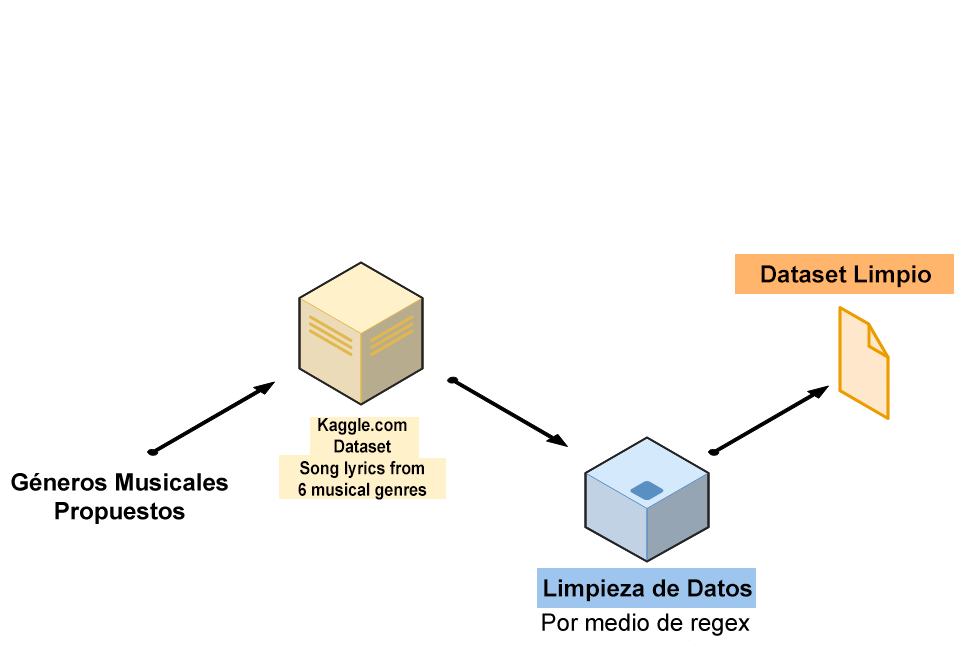
\includegraphics[scale=.4]{./imagenes/Disenio/Arquitectura/Dataset_cleaned.png}
			\caption{Diagrama de obtención de dataset}
		\end{figure}
		
		\subsection{Obtención de la base de datos}
		Para iniciar la búsqueda de la base de datos primero se eligieron las características esenciales que se muestra a continuación para poder generar el modelo:
		
		\begin{itemize}
		\item Letra de la canción.
		\item Idioma.
		\item Artista.
		\end{itemize}
		
		Se hizo la búsqueda de datasets con estás características en páginas que contienen datasets con licencia del tipo open source, tales como Kaggle \cite{kaggle}, Google datasets \cite{googleDatasets}, \acrshort{aws} Open Data \cite{awsOpenData} y en papers de investigación.\\\\
		Encontramos diferentes datasets que contaban con algunas de las necesidades del sistema pero por una u otra razón no se podían utilizar, tal fue el caso del dataset de Music4All \cite{music4all} que contaba con las necesidades del sistema pero el uso de los datos era muy restringido.\\

		En Kaggle \cite{kaggle} se encontró un dataset llamado “Song lyrics for 6 musical genres" \cite{kaggleDataset} el cual contiene todos los datos necesarios para el sistema con un total de 160,790 letras de canciones con las tablas mostradas a continuación:\\\\
		\begin{figure}[H]
			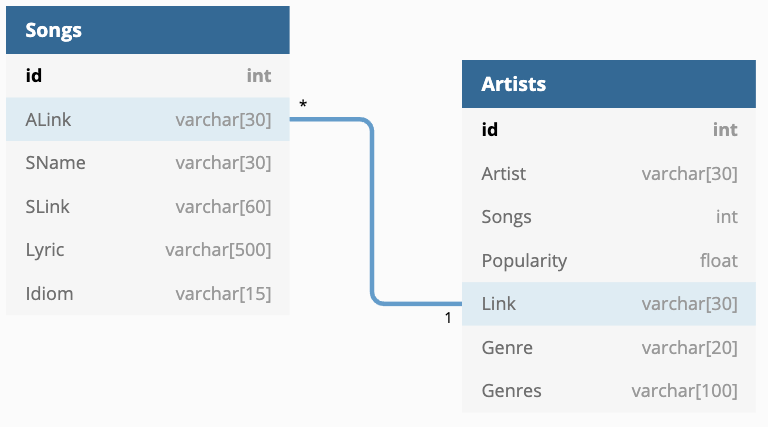
\includegraphics[width=12cm]{./imagenes/Disenio/Iteracion_1/Base_de_Datos/diagrama_ER_BD.jpg}
			\centering 
			\caption{Diagrama entidad-relación de la base de datos}
		\end{figure}
		Dicha base de datos se sacó originalmente de la página de vagalume.com \cite{vagalume} e incluye 6 tipos de géneros musicales mencionados a continuación, los cuales son:
		\begin{itemize}
			\item Rock
			\item Pop
			\item Hip Hop
			\item Samba
			\item Sertanejo
			\item Funk Carioca
		\end{itemize}
	
		Se cuenta con dos tablas que cumplen con las características ideales para realizar el modelo acorde a los requerimientos funcionales.\\\\
		Como se puede observar, se tienen las columnas “Genre” que utilizaremos para separar el dataset en géneros musicales y “Link” que servirá como enlace a la segunda tabla.\\\\
		Se utilizarán las columnas de “Lyric” para poder entrenar el modelo, “Idiom” para seleccionar y utilizar las canciones en el idioma inglés y “ALink” que nos servirá para fusionar la tabla mencionada anteriormente con la actual y así poder usar esas columnas, quedando un resultado como en la siguiente figura:
		\begin{figure}[H]
			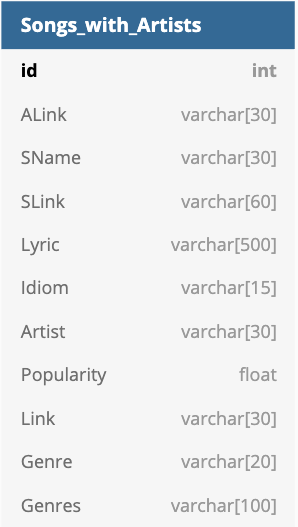
\includegraphics[width=5cm]{./imagenes/Disenio/Iteracion_1/Base_de_Datos/Songs_with_Artists.png}
			\centering 
			\caption{Diagrama entidad-relación de la base de datos procesada}
		\end{figure}
		\subsection{Género musical} % Explicar por qué se sacó de este género musical
		El género musical que elegimos es Pop en inglés debido a que es un género musical flexible en su estructura y en su léxico, otros géneros contemplados fueron Hip Hop y Rock que también cuentan con un extenso catálogo de datos pero se encontraron modelos que ya utilizan esos géneros.
		
		\subsection{Resultados}
		Al necesitar extraer información precisa para el entrenamiento del modelo no es necesario que la base de datos sea muy compleja, razón por la cual las tablas mostradas en el diagrama entidad-relación se ve así, siendo lo de mayor relevancia el mostrar que un artista puede tener muchas canciones pero una canción le pertenece únicamente a un artista.
		\begin{figure}[H]
			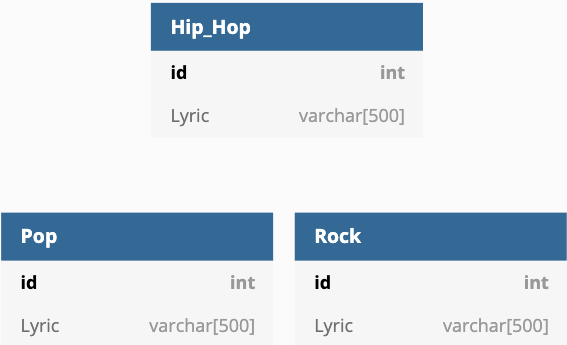
\includegraphics[width=10cm]{./imagenes/Disenio/Iteracion_1/Base_de_Datos/Hip_Hop.png}
			\centering 
			\caption{Diagrama entidad-relación final}
		\end{figure}
		
		
\newpage
%%%%%%%%%%%%%%%%%%%%%%%%%%%%%%%%%%%%%%%%%%%%%%%%%%%%%%%%%
%                                                       																																		  %
%                                                      																																	  		  %
%              																	 Iteración 2 																				  			 %
%                                                      																																			  %
%                                                      																																			  %
%%%%%%%%%%%%%%%%%%%%%%%%%%%%%%%%%%%%%%%%%%%%%%%%%%%%%%%%% 
	
	\section{Limpieza de la base de datos} % Explicar cómo se limpió la base de datos
		\subsection{Descripción}
		Una vez obtenida la base de datos, es necesario hacer una inspección de esta misma para verificar que los estos datos sean útiles para proceder a generar un modelo, este paso resulta de suma importancia, ya que de esto depende que la precisión de los resultados del modelo.\\\\
		Para ello se identificarán datos que resulten incompletos, incorrectos, inexactos, no pertinentes para
		luego sustituirlos, modificarlos o en su caso, eliminar estos datos.\\\\
		Una vez realizada esta limpieza, la base de datos será compatible con el entrenamiento y los resultados generados al final serán más entendibles.\\\\
		Estas inconsistencias en el conjunto de datos pueden ser causados por errores de entradas del usuario, corrupción de los datos, errores en el área de scraping, o simplemente tienen caracteres que no nos interesa procesar.\\\\
		
		Se utilizará la librería de “Pandas” y en caso de que se requiera, utilizar la librería de expresiones regulares para hacer esta limpieza, estás dos librerías de Python ayudarán a que los datos puedan ser utilizados para realizar el debido preprocesamiento como siguiente paso sin tener que cambiar cada campo manualmente, lo que mejora la eficiencia para poder lograr el objetivo propuesto.\\\\
		Para limpiar los datos seguiremos el estándar de limpieza de datos:\cite{data_cleaning}
		
		\begin{enumerate}
			\item Remover caracteres innecesarios
			\item Eliminar Duplicados
			\item Evitar errores ortográficos de similitud
			\item Convertir los tipos de dato
			\item Tratar los valores nulos o faltantes
		\end{enumerate}
		\newpage
		\subsection{Remover caracteres innecesarios} 
		Es necesario remover este tipo de elementos del conjunto de datos para que al momento de entrenar el modelo, no arroje resultados con valores ilegibles o incluso, que no se pueda tratar la base de datos correctamente.\\\\
		Para este paso, es necesario tener conocimiento de expresiones regulares básicas para poder delimitar los espacios dobles, letras o caracteres especiales ilegibles, saltos de línea, tabuladores, entre otros que puedan causar errores en los siguientes pasos.
		
		\subsection{Eliminar duplicados} 
		Pueden existir datos duplicados dentro de la base de datos que para el entrenamiento sería inútil además que solicitaría recursos innecesarios al sistema el meter más datos de los necesarios, para ello, con la función drop.duplicates() de pandas, se podrá lograr el acometido sin problema alguno.
		
		\subsection{Evitar errores ortográficos o de similitud}
		Existen librerías en el idioma inglés para corregir la ortografía, en este proyecto se quiere generar la letra apegada a la jerga utilizada en el idioma para poder generar las nuevas letras de canciones, por lo que no será necesario hacer a profundidad este paso.
		
		\subsection{Convertir los tipos de dato} 
		Se va a corroborar que todas las celdas contengan únicamente el tipo varchar con un límite de 500 caracteres, número elegido al tener una media de todos los elementos de 350 caracteres aproximadamente. El número de filas que contienen más de 500 caracteres es muy bajo por lo que al cortar las canciones que tienen más puede ayudar a ahorrar la memoria utilizada a la hora del entrenamiento.
		\subsection{Tratar los valores nulos o faltantes} 
		Tener datos nulos en el entrenamiento puede llegar a ser fatal debido a que además de utilizar demasiada memoria, a la hora de generar resultados, estos resultan en nulos, además que tratar la misma base de datos a la hora del preprocesamiento puede arrojarnos errores a la hora de manipular la base de datos.
		
		\subsection{Resultados} % Explicar los Resultados
		Una vez realizada esta limpieza general del conjunto de datos, el resultado esperado es tener una base de datos útil y solo con los datos necesarios para poder tratarlos con el debido proceso para empezar el preprocesamiento de entrenamiento del modelo de la red neuronal, este proceso es necesario hacer solo una sola vez para cada género musical ingresado, en caso de que se lleguen a necesitar más datos, será necesario repetir el proceso para poder generar resultados de la manera más óptima posible.
		A continuación se muestran las primeras líneas de la base de datos limpias.
		\begin{figure}[H]
			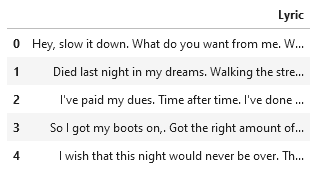
\includegraphics[width=7cm]{./imagenes/Disenio/Iteracion_2/Base_de_Datos/ResultadosLimpiezaBasedeDatos.png}
			\centering 
			\caption{Resultados de limpieza en la base de batos}
		\end{figure}
\newpage

%%%%%%%%%%%%%%%%%%%%%%%%%%%%%%%%%%%%%%%%%%%%%%%%%%%%%%%%%
%                                                       																																		  %
%                                                      																																	  		  %
%              							Iteración 3  																				  			 %
%                                                      																																			  %
%                                                      																																			  %
%%%%%%%%%%%%%%%%%%%%%%%%%%%%%%%%%%%%%%%%%%%%%%%%%%%%%%%%%
	\section{Redes neuronales a utilizar} % Explicar cómo se limpió la base de datos
		\subsection{Descripción}
		En este apartado expondremos las herramientas pensadas para el desarrollo del modelo de red neuronal, así como la manera en que podrían integrar a nuestro proyecto y las conexiones que puede tener tanto con la base de datos como con el servidor en la nube o la interfaz web. 
		\subsection{Redes neuronales para generar el modelo} % Explicar qué es una regular expression, cómo se genera y para qué sirve
		Se decidió trabajar con un modelo generado por nosotros usando como base redes neuronales de tipo \acrshort{lstm} bidireccionales debido a los problemas encontrados al tratar de usar \acrshort{bert}, este tipo de redes se pueden entrenar e ir ajustándolas hasta obtener resultados que consideremos satisfactorios. Al contar con la característica de ser bidireccional esta puede analizar el texto anterior para poder generar el texto futuro.
		
		\subsection{Modelo} % Explicar como se obtuvo en código la base de datos limpia
		
		Para el diseño del modelo se tiene contemplado el siguiente modelo del cual se puede decir que una vez se tiene la salida del transformer se pasa por una capa de clasificación, posterior a ello se usa la función “Softmax" de Python para calcular la probabilidad de aparición de cada palabra que se tiene en el vocabulario y cuyo resultado final determinará la palabra usada para la máscara (marcada de color rojo).
		\\\\
		\begin{comment}
		En última instancia, y de acuerdo a la probabilidad de rima dada por el usuario en la interfaz web, la última palabra puede o no contener una rima que haga juego con alguna de las palabras de la oración previa del verso.
		\end{comment}		
		
		\begin{figure}[H]
			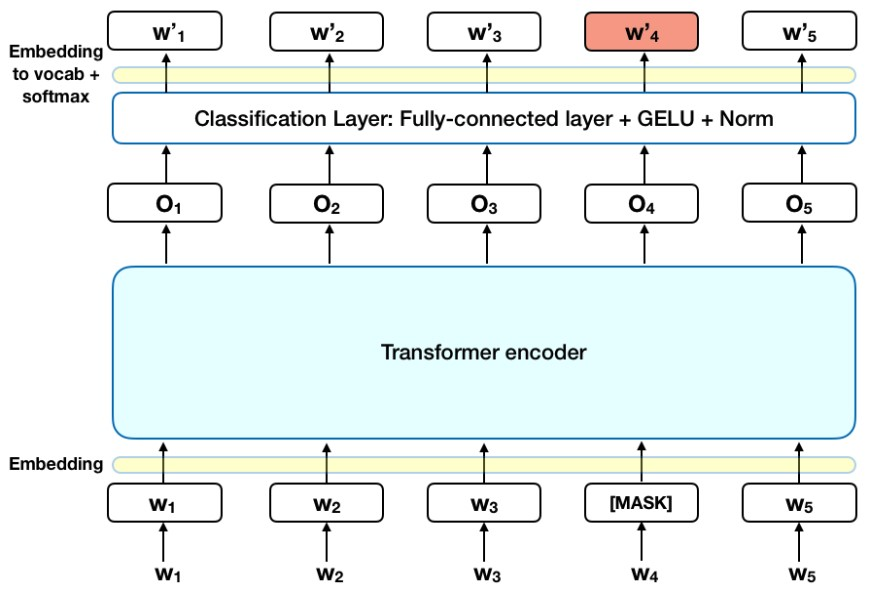
\includegraphics[width=12cm]{./imagenes/Disenio/Iteracion_3/bert_preoutput_model.jpg}
			\centering 
			\caption{Diagrama de diseño del modelo}
		\end{figure}
		
		\subsection{Resultados} % Explicar los Resultados
		
		Habiendo hecho el análisis del modelo anterior y tomándolo como referencia para nuestro proyecto podemos adaptarla de forma tal que las entradas sean en su mayoría [MASK] las cuales serán las palabras predichas siendo la razón por la cual todas las derivadas de ésto están en rojo ya que representan una entradas del tipo MASK. 
		
		
		Siendo el resultado esperado uno muy similar a la estructura que se muestra a continuación y en la que se puede ver lo siguiente:\\
		\begin{figure}[H]
			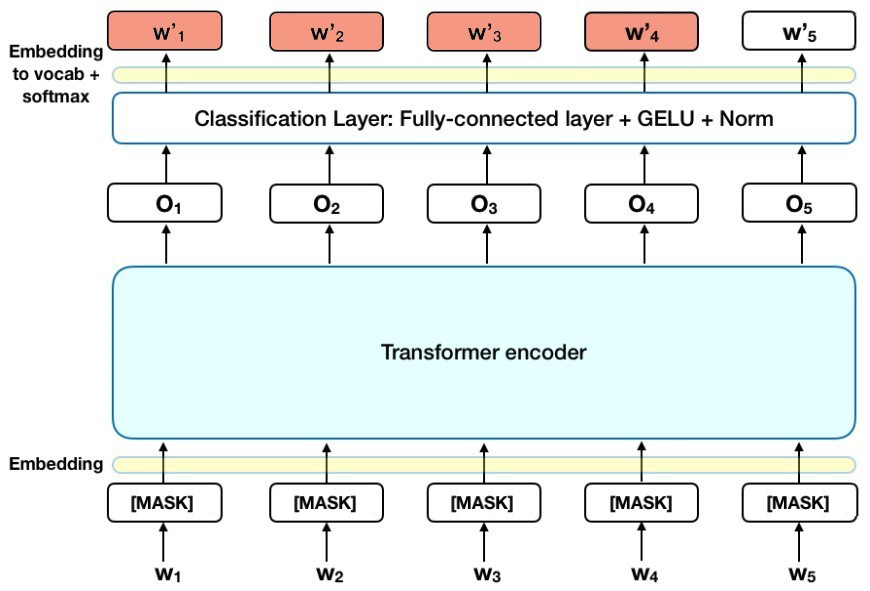
\includegraphics[width=12cm]{./imagenes/Disenio/Iteracion_3/bert_output_model.png}
			\centering 
			\caption{Diagrama de diseño final del modelo}
		\end{figure}
	
		\begin{comment}
		En todos los casos la palabra que rime tendrá un valor entre 0 y 1 (valor flotante) el cual determinará qué tan alta sería la posibilidad de que la palabra rime, siendo el valor 0 que no rime y el valor 1 representaría una rima segura. \\
		\end{comment}
		
		La estructura de las letras musicales generadas se planea que sean de la siguiente forma:		
		
		\subsubsection*{Verso}
		\begin{itemize}
			\item Estará compuesto de 4 a 6 oraciones y el valor será decidido por un número al azar.
			\item Las palabras que serán predichas en todo el verso serán de 4 a 5 y el valor será decidido por un número al azar.
		\end{itemize}
		
		\subsubsection*{Pre-coro y puente}
		\begin{itemize}
			\item Estará compuesto de 2 a 3 oraciones y el valor será decidido por un número al azar.
			\item Las palabras que serán predichas en todo el verso serán de 6 a 10 y el valor será decidido por un número al azar.
		\end{itemize}
	
		\subsubsection*{Coro}
		\begin{itemize}
			\item Estará compuesto de 3 a 4 oraciones y el valor será decidido por un número al azar.
			\item Las palabras que serán predichas en todo el verso serán de 3 a 8 y el valor será decidido por un número al azar.
		\end{itemize}
		
		\begin{figure}[H]
			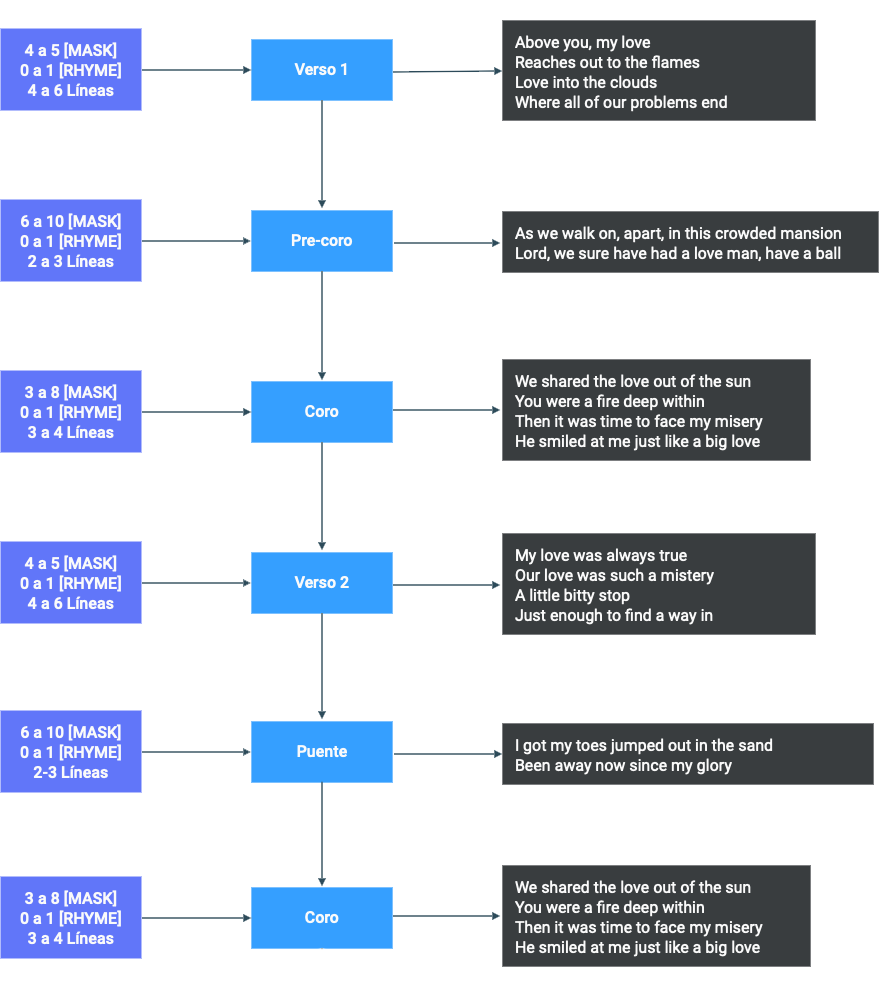
\includegraphics[width=15cm]{./imagenes/Disenio/Arquitectura/Generacion_letras.png}
			\centering 
			\caption{Diseño de la estructura del modelo}
		\end{figure}
		
		\newpage
	%%%%%%%%%%%%%%%%%%%%%%%%%%%%%%%%%%%%%%%%%%%%%%%%%%%%%%%%%
	%                                                       																																
	%
	%                                                      																																	  		  %
	%              																	 Iteración 4  																				  			 %
	%                                                      																																			  %
	%                                                      																																			  %
	%%%%%%%%%%%%%%%%%%%%%%%%%%%%%%%%%%%%%%%%%%%%%%%%%%%%%%%%%       
	
	\section{Generación del modelo en la nube} % Explicar cómo se limpió la base de datos
	\subsection{Descripción}
	
	En este apartado se hablará de las herramientas que utilizaremos, la interacción entre el desarrollador y el sistema para suministrar la base de datos a Amazon Sagemaker, el desarrollo que seguirá \acrshort{aws} para ir desde el entrenamiento del modelo hasta el despliegue del mismo para poder ser utilizado.
	El diagrama a continuación muestra el funcionamiento general para este capítulo:
	\begin{figure}[H] 
		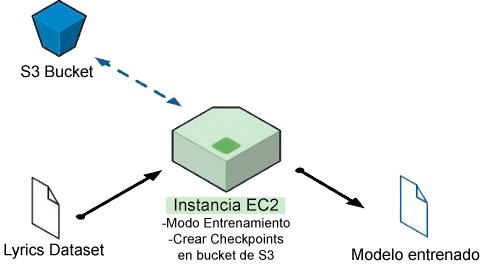
\includegraphics[scale=.75]{./imagenes/Disenio/Arquitectura/Instancias.png}
		\caption{Diagrama de instancias de AWS}
	\end{figure}
	Como se observa, ingresará la base de datos generada y se utilizará una instancia EC2, que a su vez usará en caso de necesitar más recursos un bucket de S3 para crear checkpoints resultando con el modelo entrenado a través de un número dado de epochs.
	\subsection{Amazon Sagemaker}
	Amazon SageMaker es un servicio que ayuda a científicos y desarrolladores a construir, entrenar e implementar de manera rápida y sencilla modelos de machine learning. SageMaker suprime las tareas difíciles y tediosas de cada paso del proceso de machine learning para que sea más fácil crear modelos de alta calidad.\\\\
	Dentro de las virtudes de SageMaker, y razón por la cual lo preferimos sobre la competencia, es que cuenta con 2 herramientas esenciales las cuales nos servirán al momento de entrenar el modelo:
	\begin{itemize}
	\item SageMaker Experiments: Ayuda a organizar y rastrear iteraciones en los modelos de aprendizaje automático al capturar los parámetros de entrada, configuraciones y resultados para así guardarlos como “experimentos", permitiendo que de forma posterior se pueda llevar una línea de tiempo de lo que ha sucedido y comparar estos resultados de una manera visual.
	\item SageMaker Debugger: Registra métricas del entrenamiento en tiempo real, genera advertencias y consejos de solución cuando se detectan problemas de entrenamiento comunes, así como monitorea los recursos del sistema para brindar recomendaciones respecto a cómo reasignar recursos y así reducir los costos.
	\item Managed Spot Training: Es una herramienta que permite entrenar los modelos de aprendizaje automático con instancias de Amazon \acrshort{ec2} que pueden demorar más al entrenar a cambio de abaratar los costos de entrenamiento hasta en un 90\%.
	\end{itemize}
	\newpage
	
	\subsection{Suministrado de datos}
	Al ingresar a SageMaker lo primero que nos es requerido hacer es una instancia bloc de notas (Jupyter Notebook) dentro del cual escribiremos el código en Python que ocuparemos para ejecutar todo el procedimiento visto en la iteración tres.
	
		\subsubsection*{Instancia de bloc de notas}
		Dentro de Amazon Sagemaker creamos un bloc de notas (Jupyter Notebook) dentro del cual podremos operar con código Python y el cual tiene como ventaja principal el correr código por bloques evitando de esta manera el tener que reescribirlo y pudiendo correr todo de manera secuencial nuevamente o insertar nuevos bloques entre los previamente creados según veamos más conveniente.\\
		
		\begin{figure}[H]
			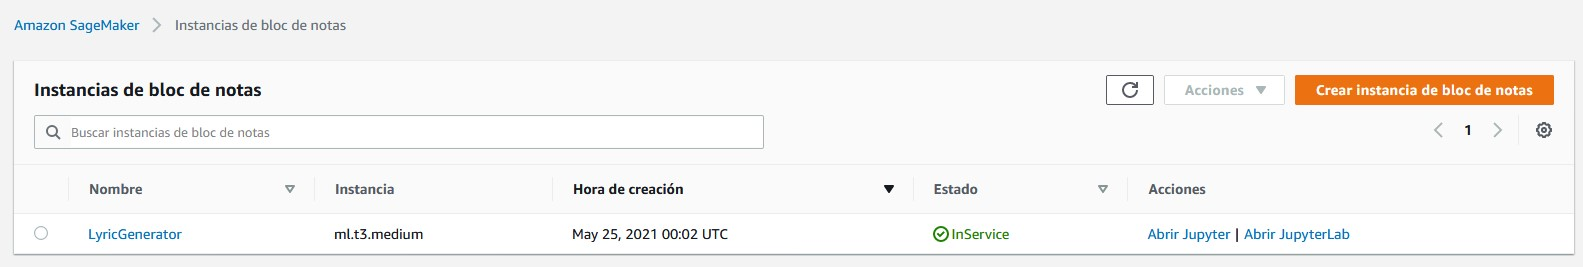
\includegraphics[width=12cm]{./imagenes/Disenio/Iteracion_4/JupyterInstance.jpg}
			\centering 
			\caption{Instancia creada en AWS}
		\end{figure}
	
	Dentro de la instancia de Jupyter se va a realizar lo siguiente:
	
	\begin{itemize}
		\item Filtrar y preparar el contenido del dataset que le proporcionemos.
		\item Entrenar el modelo, el cual podremos supervisar desde una instancia proporcionada por Amazon SageMaker durante este paso llamado “Instancia de Entrenamiento de Aprendizaje de Máquina".
		\item Generar el modelo así como dar estadísticas del mismo para poder corroborar que fue generado exitosamente.
		\item Desplegar el modelo, para este paso de la misma forma que ocurre con el entrenamiento del mismo, Sagemaker proporciona una instancia que nos permitirá alojarlo para su posterior uso llamada “Instancia de Alojamiento de Aprendizaje de Máquina".
	\end{itemize}
	
	Posterior a todos los pasos mencionados anteriormente que se realizarán dentro de la instancia en Jupyter, se puede crear ahí mismo una `\acrshort{api} endpoint' que responderá a una petición hecha por el usuario para acceder al modelo generado y así generar o devolver la letra.
	
	\begin{figure}[H]
		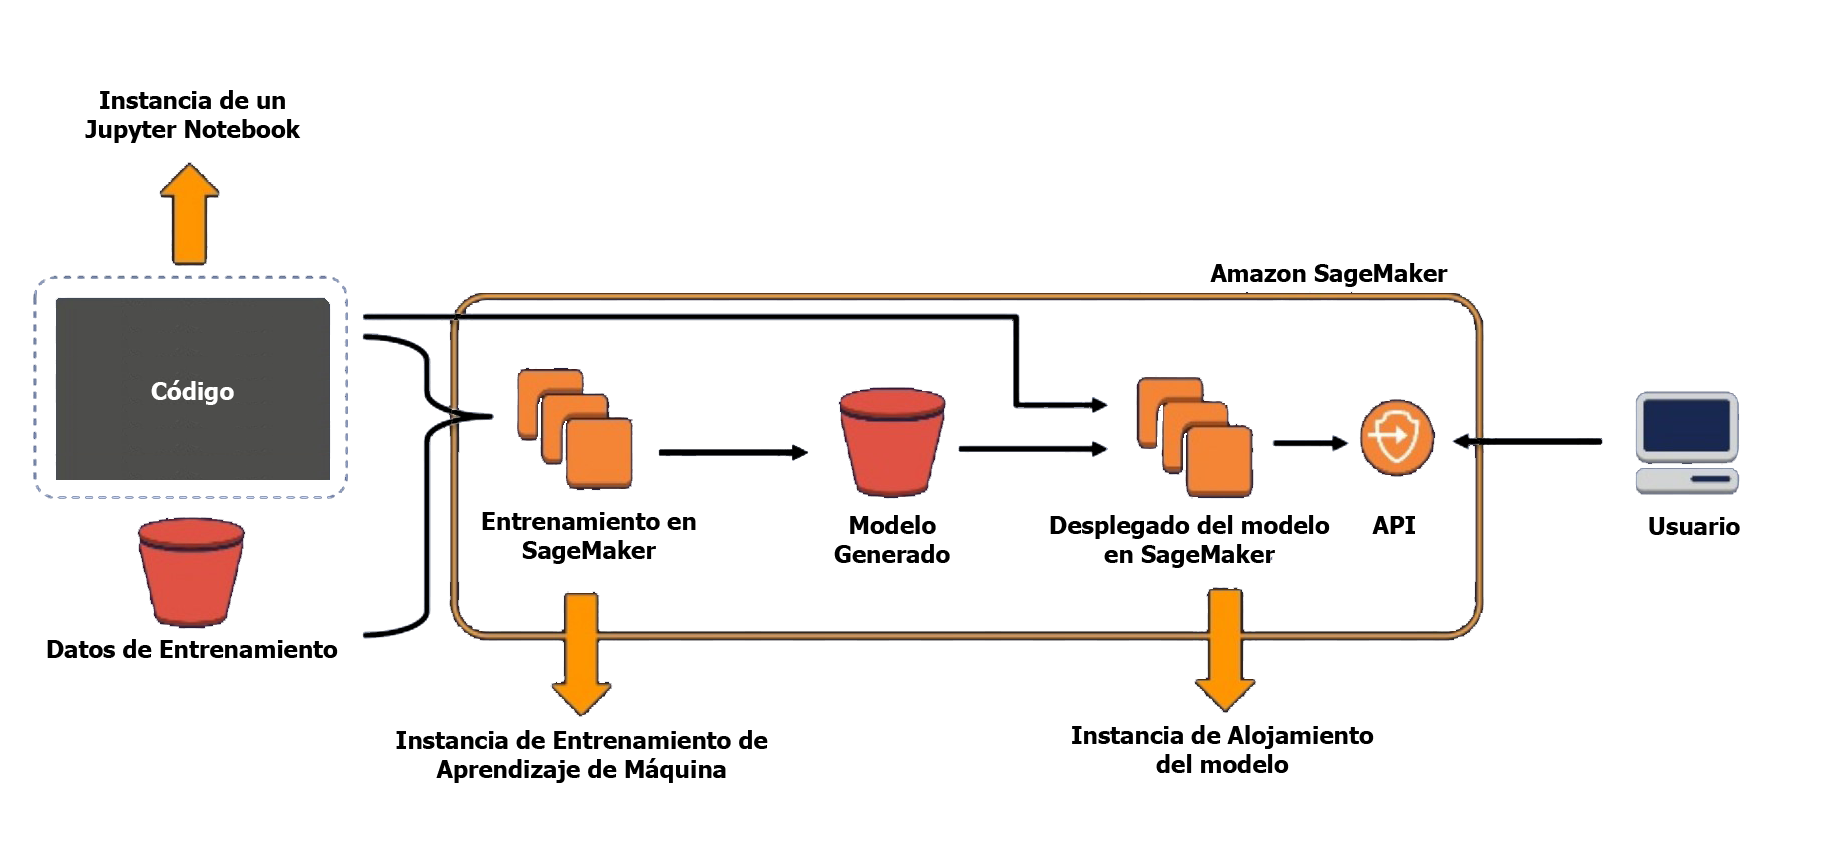
\includegraphics[width=12cm]{./imagenes/Disenio/Iteracion_4/sagemaker_function.png}
		\centering 
		\caption{Diagrama del funcionamiento de SageMaker}
	\end{figure}
	
	Como se puede apreciar en el diagrama, dentro de Amazon SageMaker ocurrirán todos los procesos que requerimos se ejecuten para poder entrenar y generar el modelo al que el usuario final podrá contactar por medio de una \acrshort{api} para solicitar la letra de una canción según sus requerimientos especificados.
	\begin{comment}
		
	Habiendo visto el proceso de alimentación de datos para el modelo podemos ahora mostrar de manera general el proceso que tomaremos para el entrenamiento de nuestro modelo, proceso que puede resumirse en el siguiente diagrama:\\\\
	A continuación se muestra el proceso seguido para el entrenamiento del modelo:
	
	\begin{figure}[H]
	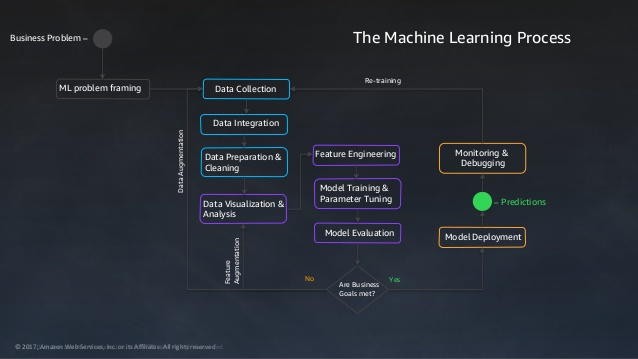
\includegraphics[width=15cm]{./imagenes/Disenio/Iteracion_4/machine_learning_process.jpg}
	\centering 
	\caption{Diagrama de diseño del modelo}
	\end{figure}
	
	Una vez se tienen los pasos necesarios para la generación del modelo podemos describir la interacción del administrador con el sistema de la siguiente manera:
	\begin{figure}[H]
	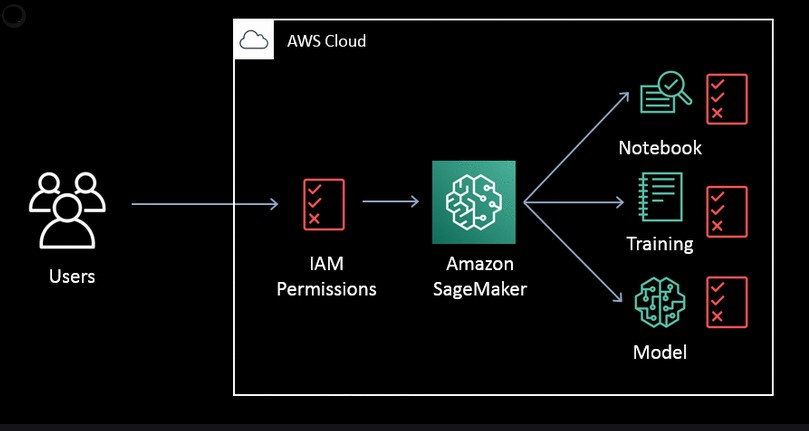
\includegraphics[width=12cm]{./imagenes/Disenio/Iteracion_4/user_interaction.jpg}
	\centering 
	\caption{Diagrama interacción del administrador con AWS}
	\end{figure}
	\end{comment}
	
	\subsection{Resultados}
	La generación del modelo de neural network utilizando herramientas en la nube, podrá ahorrar el proceso de entrenamiento cada vez que se corra algún algoritmo y teniendo acceso a herramientas proporcionadas por empresas como \acrshort{aws}, acortan de gran manera los tiempos que corriendo de forma local, tardaría bastantes horas en realizarse. El inconveniente de usar este tipo de herramientas es que si se tienen mal configuradas pueden causar grandes gastos al usuario que las utiliza. Sin embargo, se harán las pruebas pertinentes para que esto no ocurra.\\\\
	A continuación se muestra un modelo aproximado para poder generar nuestro modelo en la nube:
	\begin{figure}[H]
	
\includegraphics[width=12cm]{./imagenes/Disenio/Iteracion_4/resultado_arquitectura.png}
	\centering 
	\caption{Diagrama simple del proceso seguido para generar el modelo en la nube}
	\end{figure}
	
	\newpage

\section{Aplicación web}
\begin{figure}[H] 
	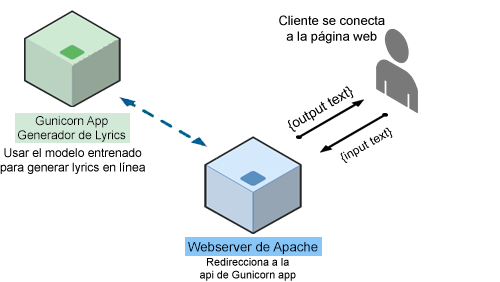
\includegraphics[scale=.75]{./imagenes/Disenio/Arquitectura/Usuario_modelo.png}
	\caption{Diagrama de conexión entre modelo y usuario}
\end{figure}
La figura anterior, muestra el funcionamiento general entre la aplicación del modelo entrenado para generar lyrics en línea y el usuario final accediendo a la red desde su navegador..
En este apartado se mostrará un primer boceto de las vistas que verá el usuario final en la aplicación web.	        
\begin{figure}[H] 
	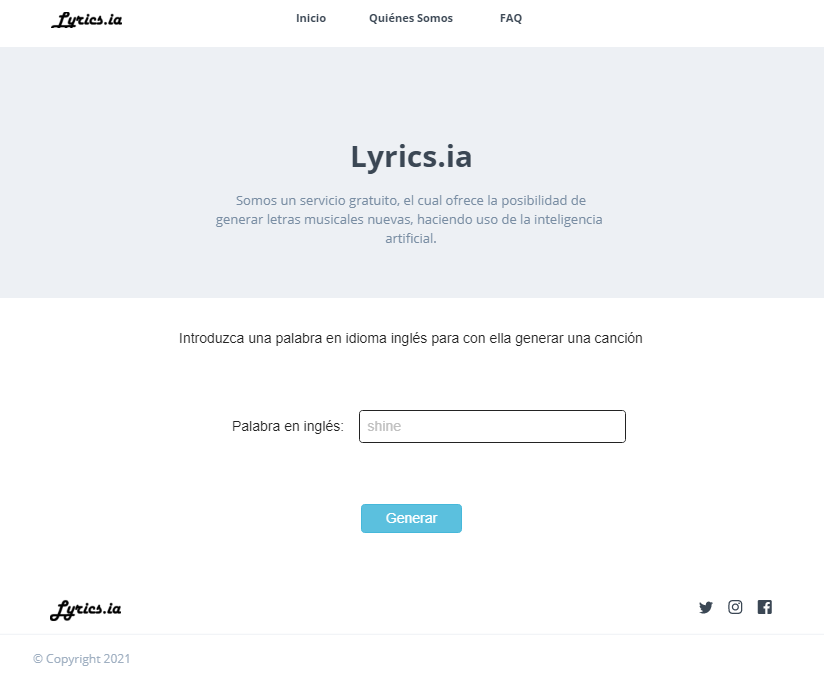
\includegraphics[width=12cm]{./imagenes/Analisis/MockFront.png}
	\centering 
	\caption{Pagina inicial que se mostrará al usuario}
\end{figure}
\begin{figure}[H] 
	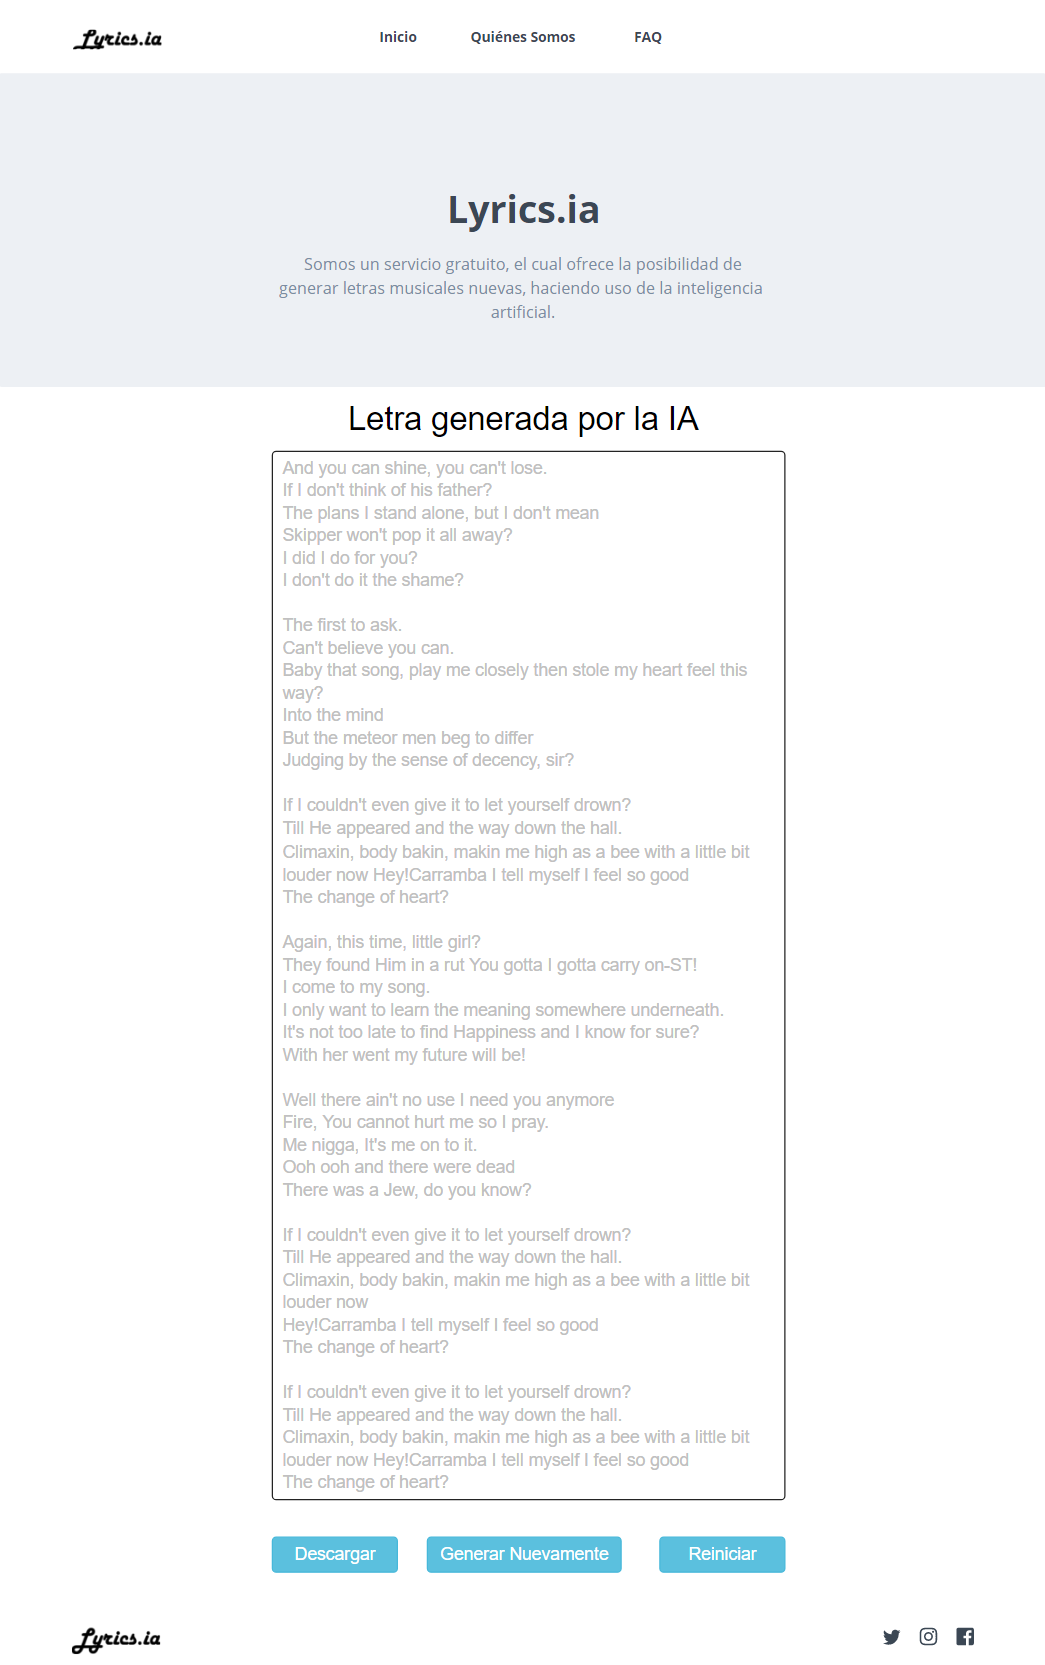
\includegraphics[width=12cm]{./imagenes/Analisis/MockFrontGenerated.png}
	\centering 
	\caption{Aplicación web, pagina una vez generada la letra musical.}
\end{figure} 

\chapter{\textcolor{azulescom}{Desarrollo}}

%%%%%%%%%%%%%%%%%%%%%%%%%%%%%%%%%%%%%%%%%%%%%%%%%%%%%%%%%
%                                                                                                                                                                                                 %
%                                                                                                                                                                                                 %
%                                                                Desarrollo del Sistema                                                                                    %
%                                                                                                                                                                                                 %
%                                                                                                                                                                                                 %
%%%%%%%%%%%%%%%%%%%%%%%%%%%%%%%%%%%%%%%%%%%%%%%%%%%%%%%%%
\section{Desarrollo del modelo}

A continuación, explicaremos la herramienta que se utilizó para desarrollar el modelo de generación de letras musicales.

\subsection{Amazon AWS}


Originalmente se planeaba trabajar con Amazon AWS, pero al momento de crear las máquinas virtuales donde se iba a laborar con la creación del modelo, nos encontramos con la problemática de que, para realizar algunas acciones, los comandos requeridos para estas tenían un cargo monetario extra a la cuenta además de lo que se invertía en mantener la máquina virtual activa.\\\\
Aunado a esto la herramienta nos amigable con el usuario, y no te brinda un manual para facilitar el manejo de esta. Por esta razón, además de ser más costoso de lo planeado se decidió cambiar de plataforma para el desarrollo del modelo.

\subsection{Google Cloud Platform}

Después se probó trabajar con la plataforma de Google la cual es similar en la creación de máquinas  virtuales a la plataforma de Microsoft Azure, esta plataforma de Google es más amigable e intuitiva para el usuario, al momento de crear tu cuenta en esta, se te otorgan 300 dólares, los cuales lo mas probable es que utilices en la maquina en la que vas a trabajar en un futuro.
\begin{figure}[H] 
	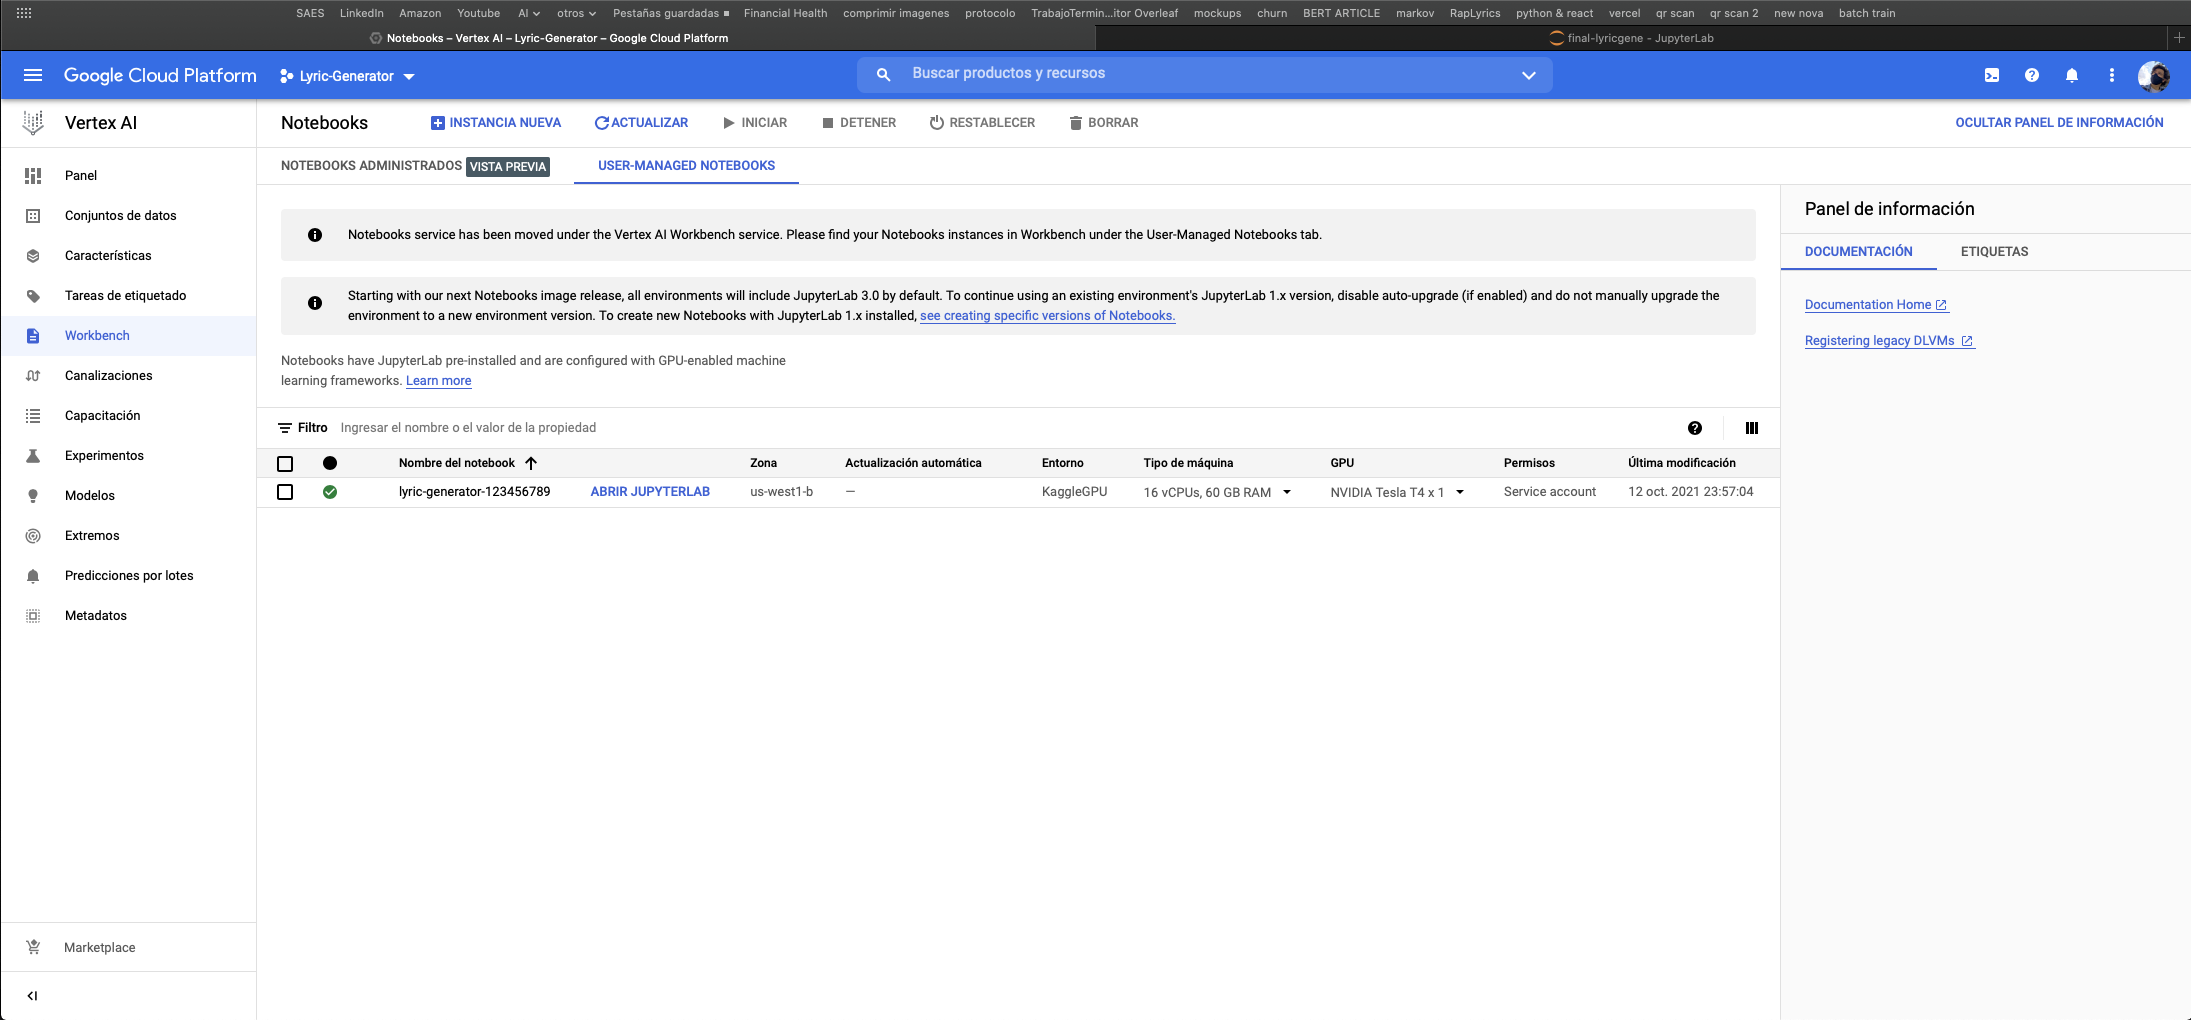
\includegraphics[width=12cm]{./imagenes/Desarrollo/Maquina.png}
	\centering 
	\caption{Máquina creada para el desarrollo del modelo.}
\end{figure}
Para el desarrollo de modelos en esta plataforma es como utilizar una libreta de Jupyter, creando una libreta en la máquina virtual que va a procesar la información y la cual va a estar trabajando con los datos del modelo, así como una cubeta donde se va a encontrar tu base de datos que el modelo va procesar, en este caso las letras de las canciones del genero pop.
\begin{figure}[H] 
	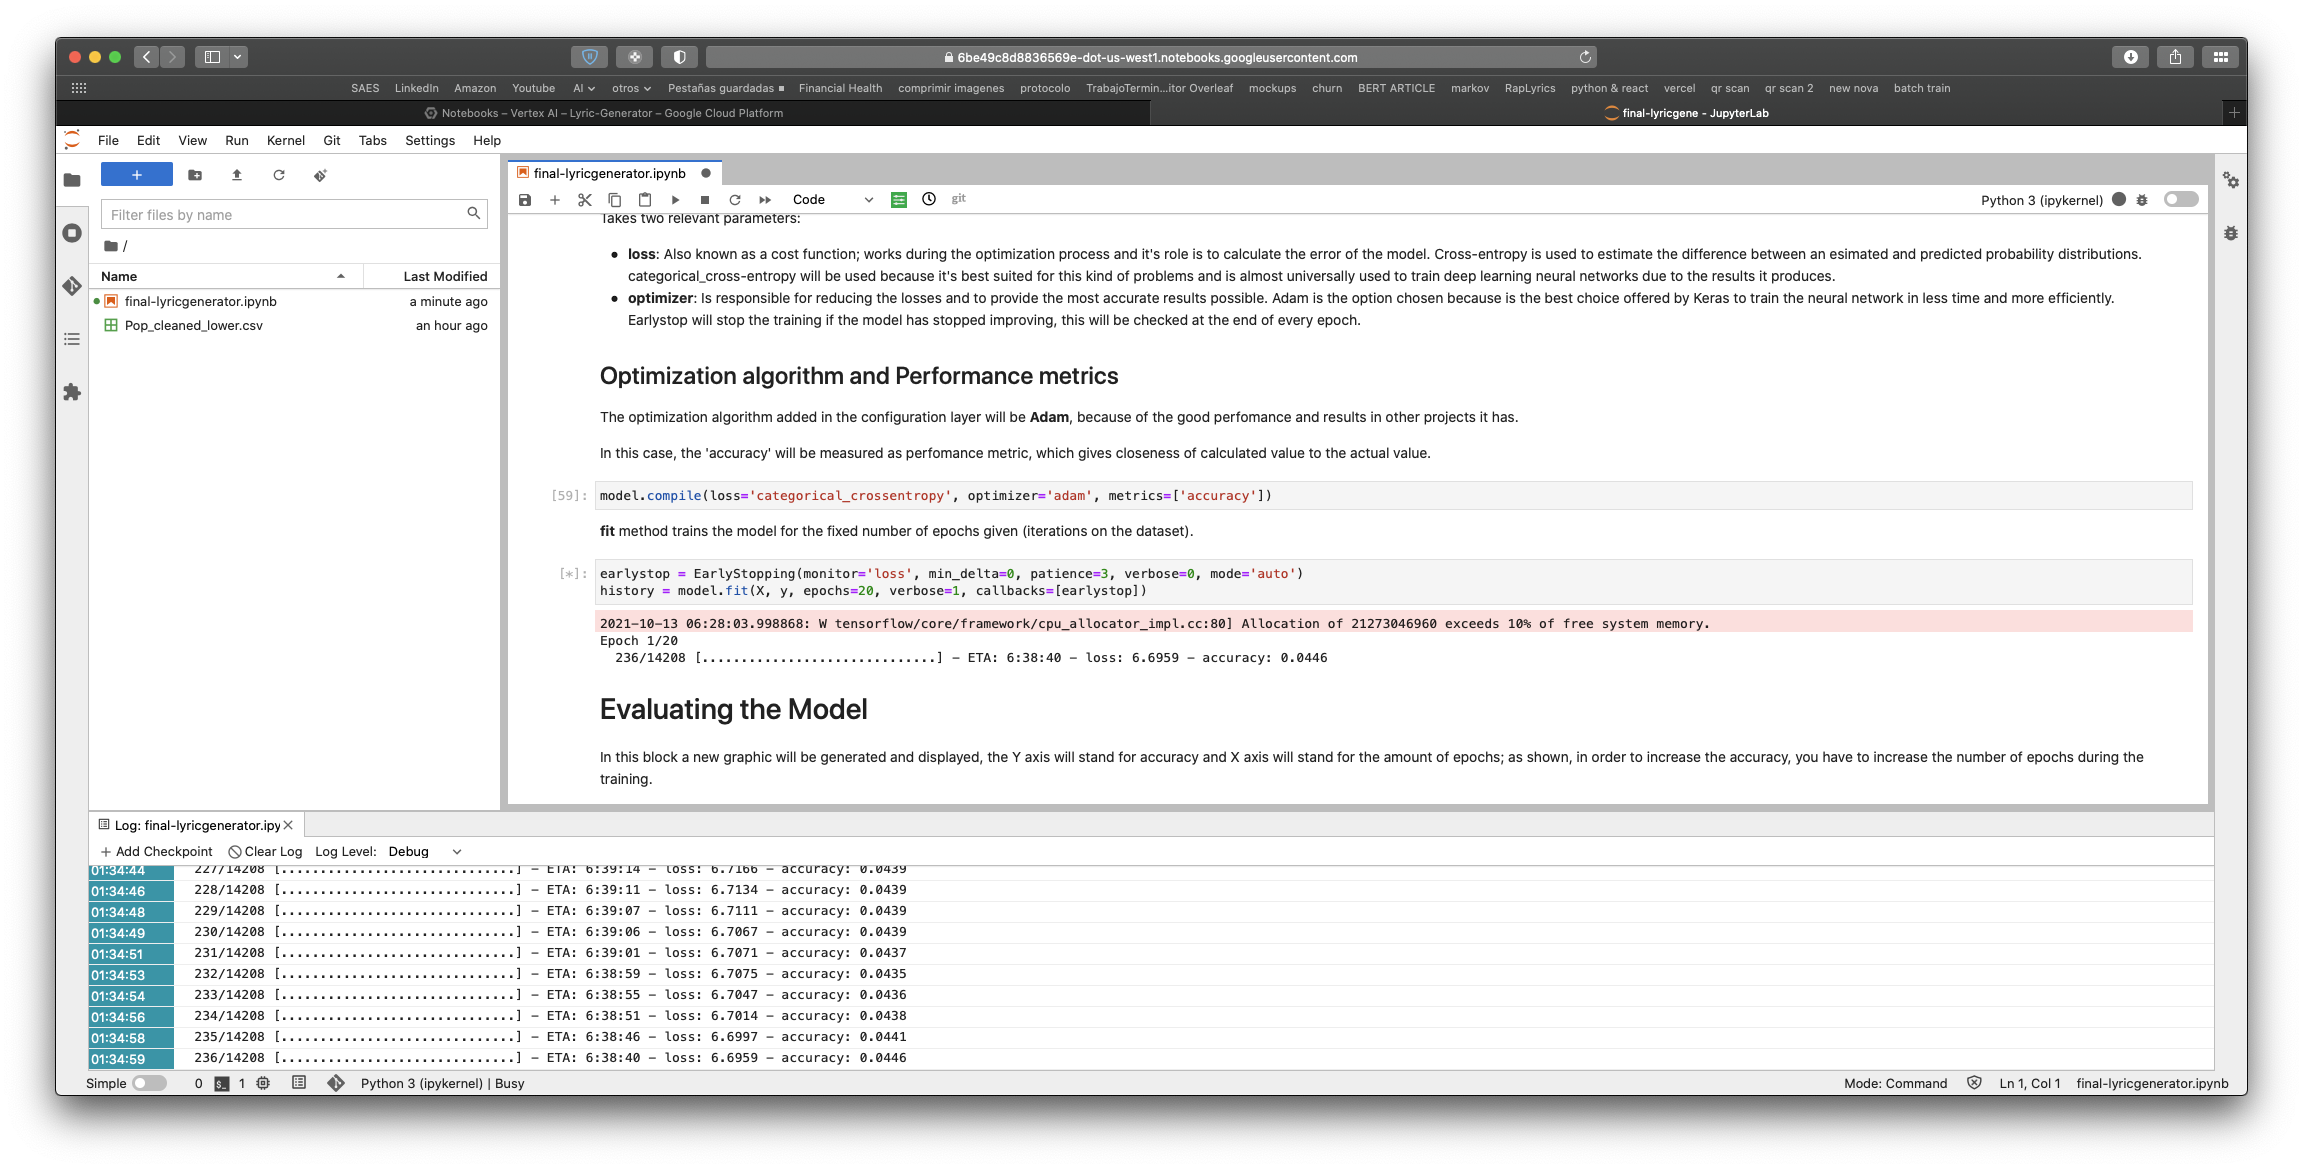
\includegraphics[width=12cm]{./imagenes/Desarrollo/Notebook.png}
	\centering 
	\caption{Libreta y entrenamiento del modelo.}
\end{figure}
\begin{figure}[H] 
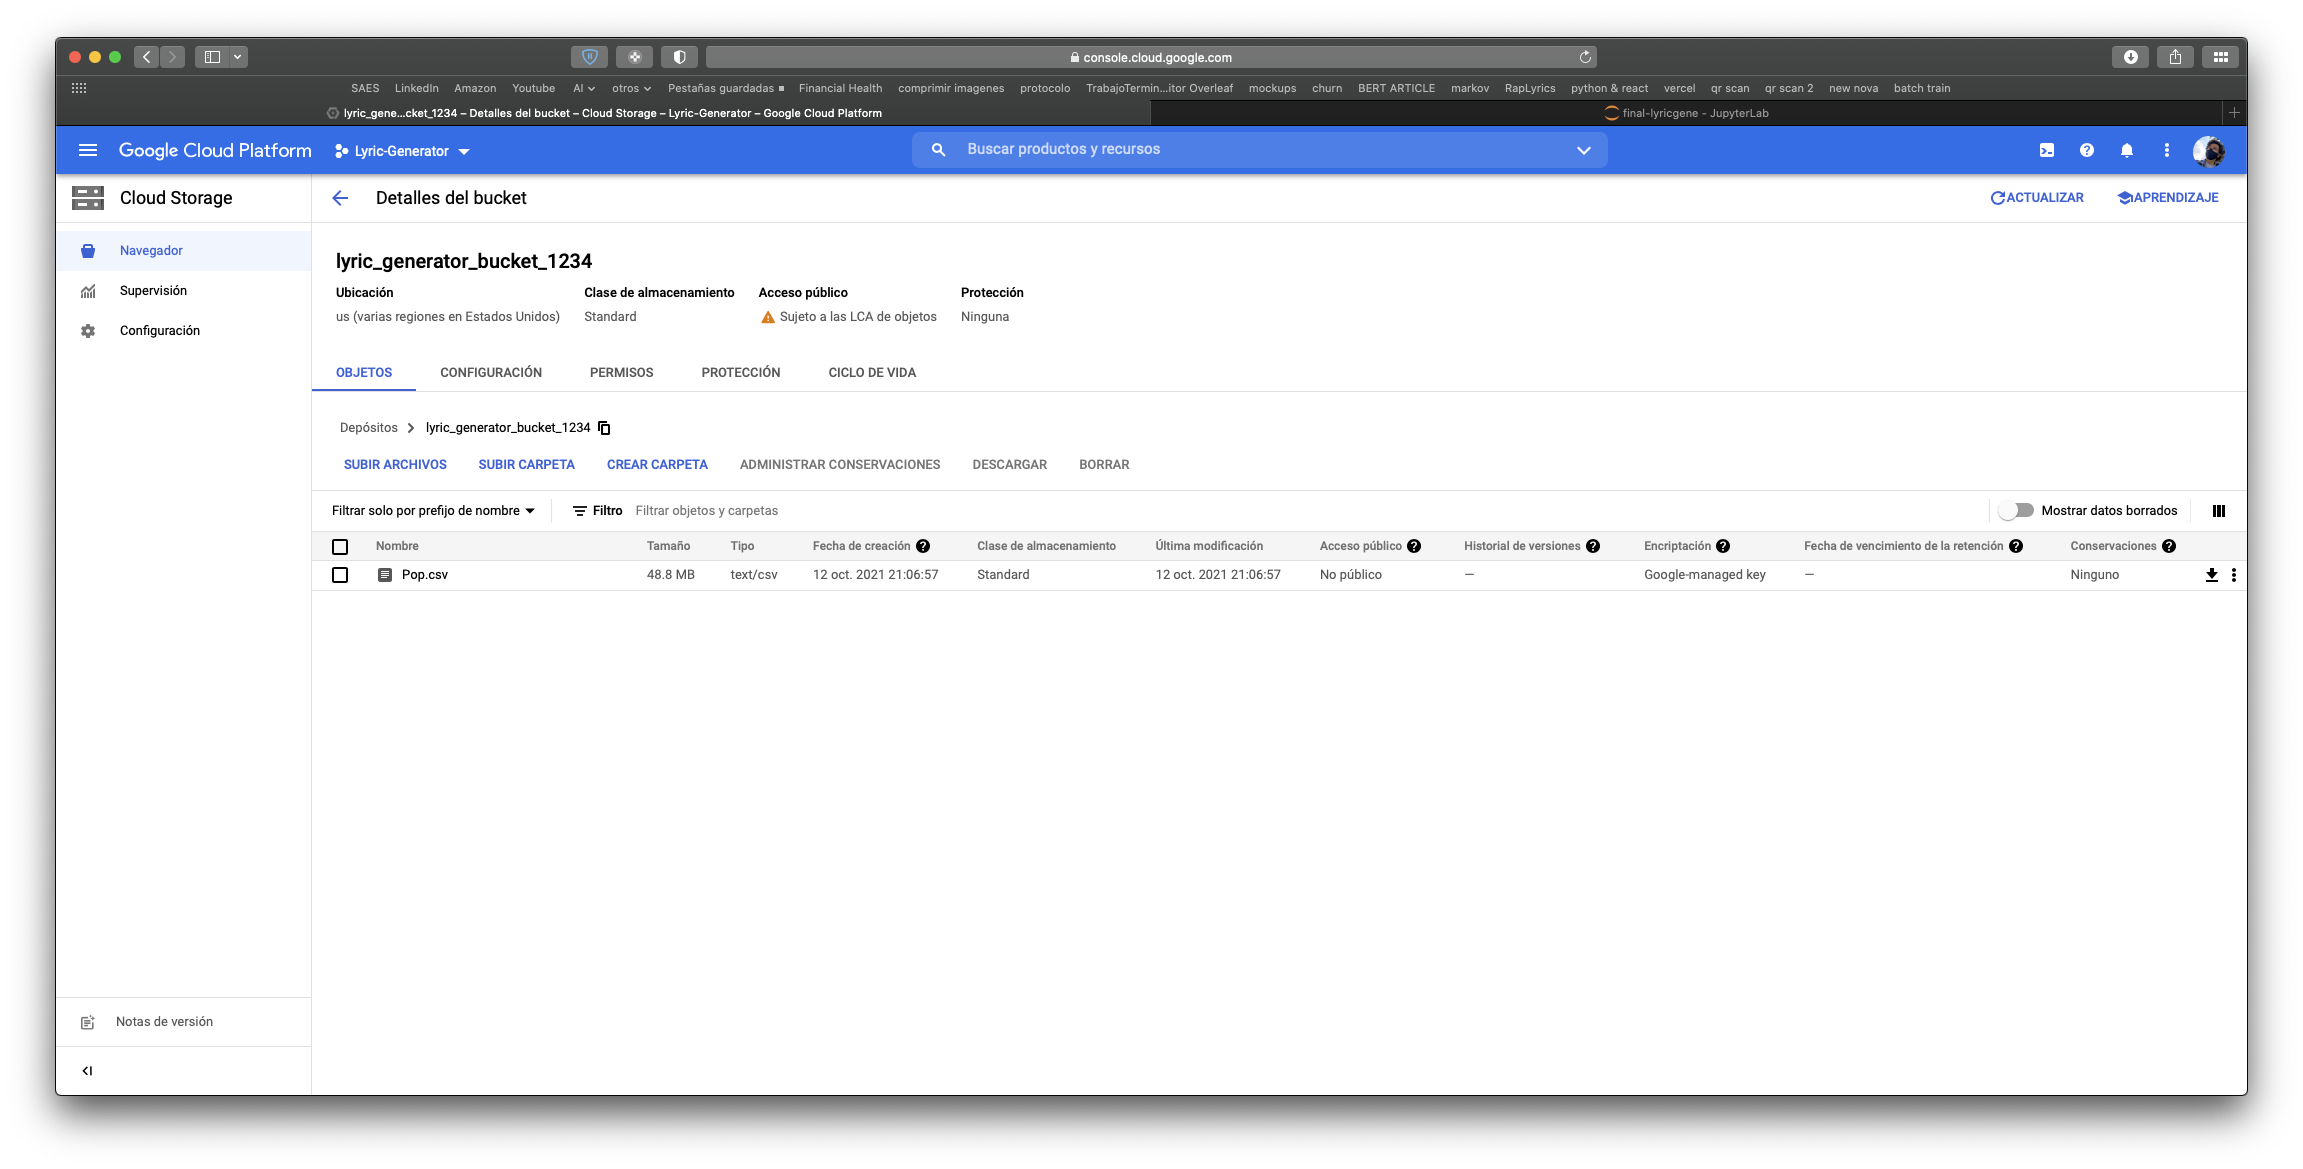
\includegraphics[width=12cm]{./imagenes/Desarrollo/Bucket.png}
\centering 
\caption{Cubeta donde se encuentra la base de datos que contiene las letras de las canciones.}
\end{figure}
No utilizamos esta herramienta al final, principalmente a que los resultados obtenidos fueron similares a los conseguidos con el modelo desarrollado en la plataforma de Kaggle, además debemos considerar que el mantenimiento de la máquina virtual en la plataforma de Google era de 265 dólares mensuales y no se cuenta con el presupuesto para este mantenimiento.

\subsection{Kaggle}

Al final de realizar prueba decidimos utilizar la plataforma de Kaggle la cual con una cuenta gratuita puedes hacer funciones similares a las presentadas en la plataforma de Google, con algunas limitantes en cuanto a los recursos que puedes emplear al momento de trabajar.\\\\
En esta plataforma también debes seleccionar los elementos con los cuales tu ambiente va a trabajar, en este caso el máximo de memoria RAM disponible era de 16Gb, un disco de 73Gb y un GPU de 13 Gb, estos recursos fueron los utilizados para el procesamiento de nuestro conjunto de datos, así como una libreta la cual va a ser el área donde vamos a estar trabajando.\\\\
Debido a las limitantes de procesamiento nos vimos en la necesidad de limitar el modelo a entrenar, en lugar de utilizar las 28441 letras de canciones del genero pop, solo se pudo trabajar con 700.\\\\
Con estas 700 lyrics, se decidió obtener información de ellas, siendo más específicos, estadísticas como el número de palabras en cada canción, esto con el fin de determinar la frecuencia de distribución del número de palabras de cada texto y para tener una idea del promedio de palabras, esto con el fin de tenerlo en cuenta al momento de realizar la generación de texto.
	\begin{figure}[H]
	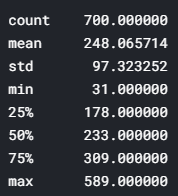
\includegraphics[width=5cm]{./imagenes/Desarrollo/Kaggle/estadistica.png}
	\centering 
	\caption{Estadísticas de las palabras}
\end{figure}
Lo que podemos observar en la imagen anterior es:
\begin{itemize}
	\item \textbf{Count:} el cual es el número de canciones analizadas.
	\item \textbf{Mean:} el promedio de palabras por canción.
	\item \textbf{Std:} la desviación estándar de las palabras.
	\item \textbf{Min:} la menor cantidad de palabras encontradas en una canción.
	\item \textbf{Max:} la mayor cantidad de palabras encontradas en una canción.
\end{itemize}
Además, se realizo una tokenizacion a las letras de nuestras 700 canciones, esto quiere decir que se separo cada palabra y cada palabra se convirtió en un número. Para este proceso se hizo uso de Keras y la clase Tokenizer(), la cual cuenta con dos métodos importantes:
\begin{itemize}
	\item \textbf{\_fit\_ontext():} El cual actualiza el vocabulario interno en función de una lista de textos determinada o, en este caso, la columna "Lyrics", donde cada entrada de la lista será un token.
	\item \textbf{\_texts\_tosequences():} El cual transforma cada texto dentro de la lista de textos proporcionados en una secuencia de números enteros; solo se considerarán las palabras conocidas por el tokenizador.
\end{itemize}	
\begin{figure}[H]
	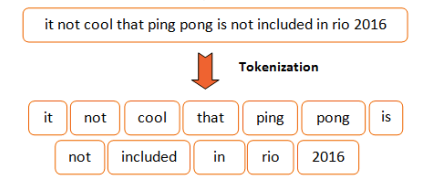
\includegraphics[width=10cm]{./imagenes/Desarrollo/Kaggle/tokenization.png}
	\centering 
	\caption{Tokenizado de las palabras \cite{tokenimagen}}
\end{figure}
Antes de la generación del modelo, es necesario normalizar todas las oraciones a una misma longitud, para evitar el desbordamiento de la memoria y conseguir que las capas del modelo sean mucho más profundas, este es un proceso simple el cual consiste en agregar ceros al comienzo del texto, dando como resultado capas del mismo tamaño.\\\\
La posición donde se sumarán los ceros viene determinada por el relleno del argumento, en este caso, se hará al comienzo de la secuencia.
\begin{figure}[H]
	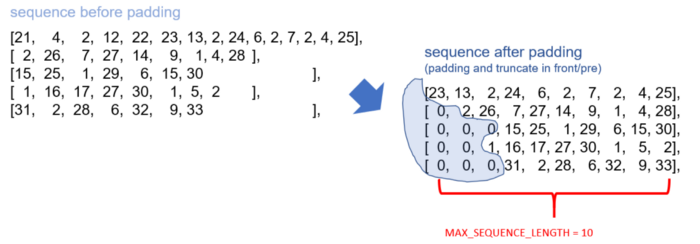
\includegraphics[width=10cm]{./imagenes/Desarrollo/Kaggle/padding.png}
	\centering 
	\caption{Padding del tokenizado de las palabras}
\end{figure}	
\newpage	
\section{Creación del modelo}
En este caso se utilizó el modelo LSTM Bidireccional, este tipo de redes neuronales se ejecutan como su nombre lo indica: en dos direcciones. Esto quiere decir que va del pasado al futuro y viceversa, así es como el modelo conserva la información de ambos estados en cualquier momento. Las redes neuronales de LSTM se utilizan principalmente cuando el contexto está involucrado.\\\\
Los modelos en Keras se definen como una secuencia de capas, y el modelo secuencial se trata de agregar capas de una en una. Las capas son el componente básico de la red neuronal.\\\\
Dentro de estas capas podemos encontrar:
\subsection{Embedding o incrustación}
Es una capa central, solo se puede usar como la primera capa en un modelo, convierte los números enteros positivos en vectores densos de un tamaño fijo (el primer parámetro es el tamaño del vocabulario, el segundo parámetro es la dimensión de la incrustación densa y el tercer parámetro es sobre la longitud de las secuencias, este se requiere ya que usaremos una capa densa más adelante)
\begin{center}
	\lstinputlisting[language=Python]{./imagenes/Desarrollo/Kaggle/embedding.py}
\end{center}
\subsection{Bidireccional}
Es una capa recurrente, una envoltura bidireccional para las redes neuronales de tipo RNN's que recibirá una capa como entrada, siendo la capa LSTM la que elegimos, recibirá un entero positivo como entrada que se refiere a la cantidad de nodos de salida que se deben devolver.
\begin{center}
	\lstinputlisting[language=Python]{./imagenes/Desarrollo/Kaggle/bidireccional.py}
\end{center}
\subsection{Dropout}
Es una capa de regularización. Esta capa establece aleatoriamente las unidades de entrada en 0, con una frecuencia del valor que le pasamos, en cada paso durante el tiempo de entrenamiento, lo que ayuda a evitar el sobreajuste.
\begin{center}
	\lstinputlisting[language=Python]{./imagenes/Desarrollo/Kaggle/dropout.py}
\end{center}
\subsection{Densidad}
Es una capa central y una capa de red neuronal densamente conectada. Recibe como primer parámetro un entero positivo que se refiere a la cantidad de nodos de salida que deben devolverse. El segundo parámetro es el llamado activación que define el tipo de predicciones que puede hacer el modelo; para el tipo de problema que estamos considerando, el que se adapta mejor es softmax, que genera un vector de valores (entrada) que puede interpretarse como probabilidades de ser utilizado.
\begin{center}
	\lstinputlisting[language=Python]{./imagenes/Desarrollo/Kaggle/dense.py}
\end{center}
\subsection{Método de compilación, algoritmo de optimización y métrica de rendimiento}
Perdida: También conocida como función de costos; funciona durante el proceso de optimización y su función es calcular el error del modelo. La entropía cruzada se utiliza para estimar la diferencia entre una distribución de probabilidad estimada y predicha. Se utilizará categorical\_cross-entropy porque es más adecuado para este tipo de problemas y se usa casi universalmente para entrenar redes neuronales de aprendizaje profundo debido a los resultados que produce.
Optimización: Se encarga de reducir las pérdidas y brindar los resultados más precisos posibles. Adam es la opción elegida porque es la mejor opción que ofrece Keras para entrenar la red neuronal en menos tiempo y de manera más eficiente. Earlystop detendrá el entrenamiento si el modelo ha dejado de mejorar, esto se verificará al final de cada epoch. En este caso, la "precisión" o “accuracy” se utilizará como métrica de rendimiento.
El método fit es el encargado de entrenar el modelo para el número fijo de epochs dados.	
\begin{center}
	\lstinputlisting[language=Python]{./imagenes/Desarrollo/Kaggle/compile.py}
\end{center}
Quedando como resultado el código del modelo de la siguiente forma:
\begin{center}
	\lstinputlisting[language=Python]{./imagenes/Desarrollo/Kaggle/modelo.py}
\end{center}
Una vez completado el entrenamiento de nuestro modelo, lo que falta es importarlo para probar cómo funciona, en nuestro caso nombramos al modelo “song\_lyrics\_generator” y se importo de la siguiente forma, llamándola a través del enlace de nuestra libreta de Kaggle:
\begin{center}
	\lstinputlisting[language=Python]{./imagenes/Desarrollo/Kaggle/import.py}
\end{center}
Ya que contemos con el modelo importado, se creó una función para generar la letra de una canción utilizando el modelo previamente entrenado, el cual predecirá las siguientes palabras en base a la palabra(s) de entrada suministradas como 'seed\_text'. Para que esto funcione, se debe aplicar una tokenización al seed\_text, luego se aplicará un relleno a las secuencias generadas y se pasará al modelo entrenado para que se pueda predecir la siguiente palabra.
\begin{center}
	\lstinputlisting[language=Python]{./imagenes/Desarrollo/Kaggle/function.py}
\end{center}	
\newpage

\section{Desarrollo del back-end}

Para el back-end se decidió trabajar con una aplicación web desarrollada en Flask, debido a que de esta era fácil y rápida de implementar, además que permitía una mejor integración con el modelo que se elaboró usando Python y la aplicación web trabajada en React.\\\\
Si se desea desarrollar una aplicación web en Flask lo primero que se tiene que hacer o que se recomienda hacer es crear un ambiente virtual usando virtualenv esto para separar nuestro entorno Python instalado originalmente del que se va a utilizar en la aplicación. Una vez realizado este procedimiento, se inició el desarrollo del código.
\begin{center}
	\lstinputlisting[language=Python]{./imagenes/Desarrollo/BackEnd/app.py}
\end{center}
El código app.py mostrado anteriormente es el código principal de nuestro back-end y es este el que se despliega en el navegador web, lo primero que se visualiza al entrar es información con respecto a esta aplicación como su nombre, versión y los plugin con los que esta cuenta.\\\\
Para poder ver un cómo es que realmente funciona el back-end se realizó una pequeña interfaz y es posible acceder a ella a través de la dirección x/swagger-ui/ en ella podemos encontrar con mayor detalle el estado actual del api, esta información se encuentra ubicada en el espacio nombrado como health.
\begin{figure}[H]
	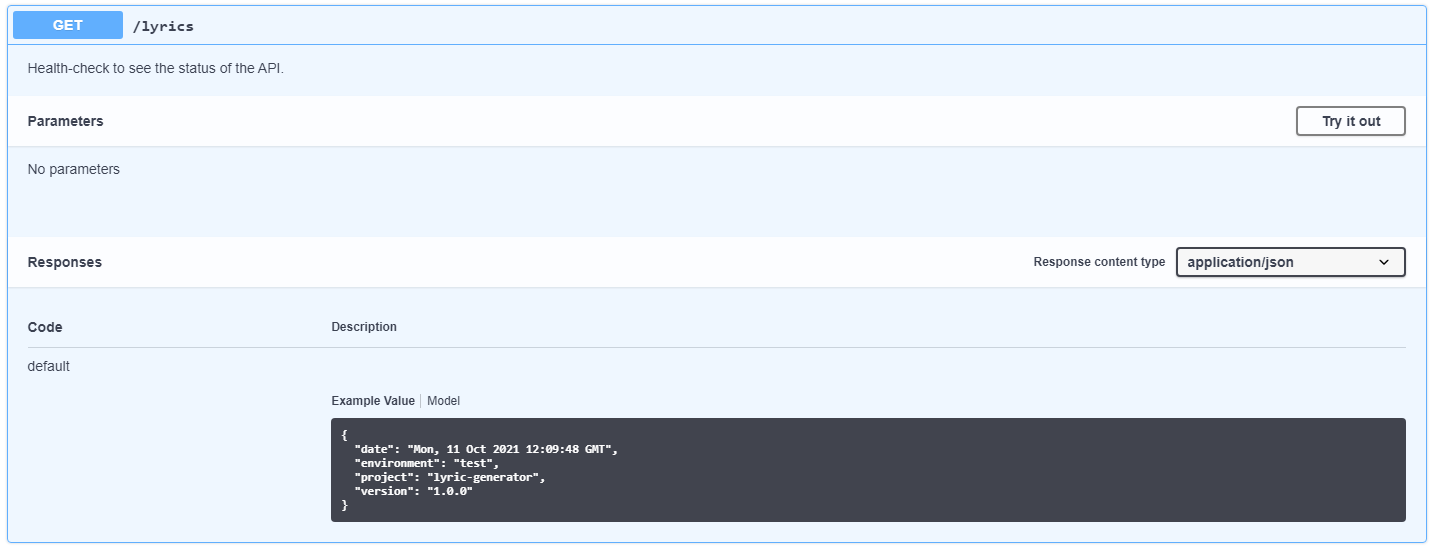
\includegraphics[width=13.5cm]{./imagenes/Desarrollo/BackEnd/Health.png}
	\centering 
	\caption{Información sobre el estado del Back-end}
\end{figure}
Un poco más abajo se encuentra el método post de la api, este es el encargado de recibir la información de la aplicación web realizada en React en formato json, siendo más específicos la palabra en inglés introducida por el usuario, para posteriormente enviar esta información al modelo.
\begin{figure}[H]
	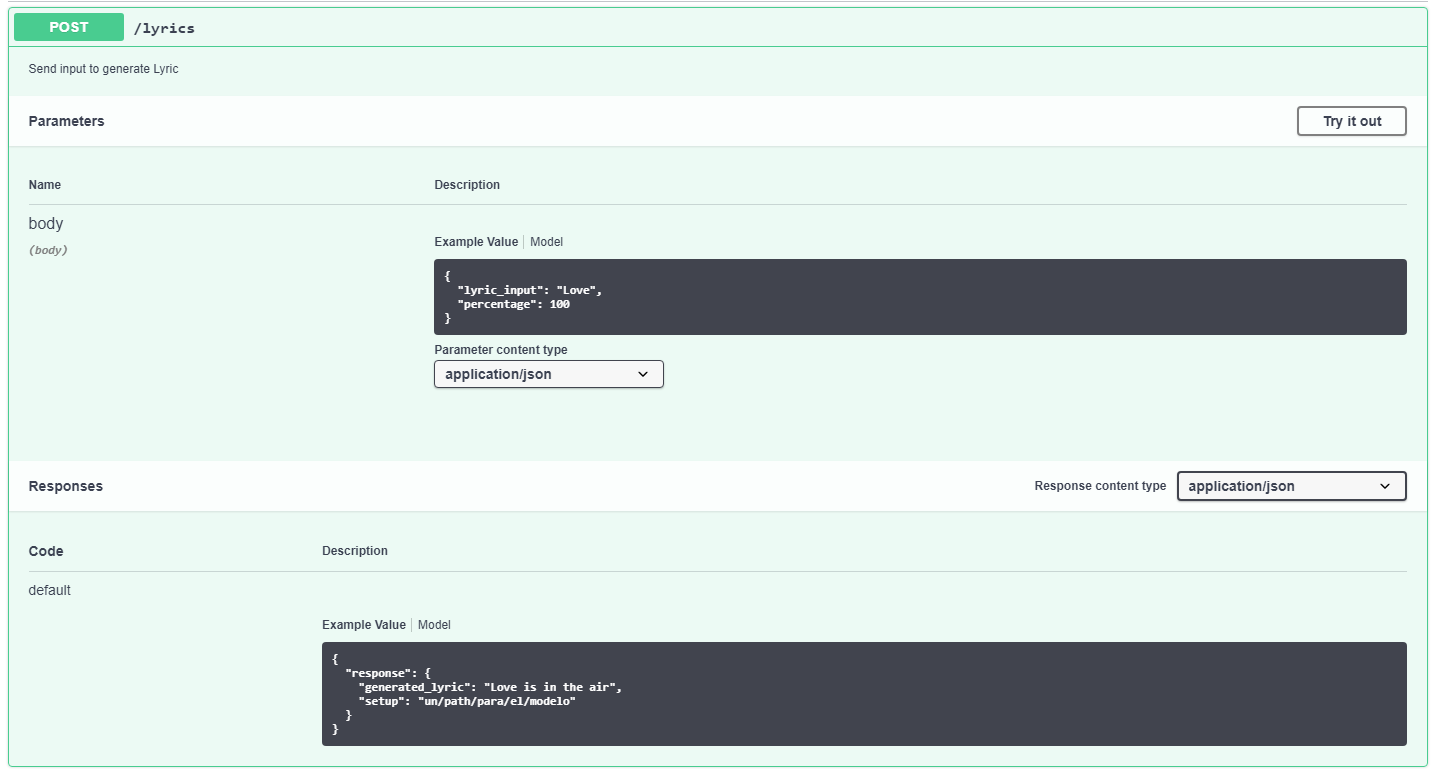
\includegraphics[width=13.5cm]{./imagenes/Desarrollo/BackEnd/Post.png}
	\centering 
	\caption{Cuadro del método Post}
\end{figure}
Para realizar la tarea más importante del proyecto, es decir, la generación del texto, se desarrolló el siguiente código:
\begin{center}
	\lstinputlisting[language=Python]{./imagenes/Desarrollo/BackEnd/generate_lyrics.py}
\end{center}
En este código lo primero que realiza es cargar el modelo previamente entrenado debido a que va a ser requerido para la generación de texto, utilizando la palabra introducida por el usuario es procesada y ocupada en nuestra clase GenerateLyric donde la palabra al igual que el resto de palabras en nuestro modelo es tokenizada y separada en caso de haber recibido mas de una vocablo, posteriormente utilizado el modelo previamente cargado y valor de la palabra tokenizada va a tratar de predecir la siguiente palabra.\\\\
Este proceso de tokenizar el texto y generar la próxima palabra a partir del valor obtenido de la tokenizacion se va a repetir hasta que se cumpla con el tamaño del verso o coro en el que se esté trabajando.\\\\
Una vez terminado con la generación del texto, es enviado a la pagina web desarrollada en React como una respuesta.

\newpage
\section{Desarrollo de la página web}
El desarrollo de la aplicación web se decidió realizarla haciendo uso de la biblioteca de Javascritpt conocida como React o ReactJS la cual consiste en crear interfaces interactivas, con la cual se puede diseñar vistas simples, en las cuales se actualizan y renderizarán los componentes necesarios cuando exista algún cambio en los datos.\\\\
Se decidió usar este recurso para el desarrollo de la página web, debido a que permite que esta sea compatible con dispositivos móviles sin la necesidad de volver a escribir código para estas tecnologías.\\\\
Para poder trabajar con React fue necesario descargar Node.js desde su página (https://nodejs.org/es/) la cual nos va a permitir crear aplicaciones web utilizando JavaScript, además de que al instalarlo obtendremos npm herramienta que posteriormente nos permitirá instalar paquetes con los cuales podemos añadir nuevas funciones a nuestra aplicación y que a su vez son compatibles con React.\\\\
Una vez que se tiene instalado Node.js, para poder ejecutar una aplicación web en terminal, debemos escribir npm start, lo cual ejecutara un servidor de desarrollo de manera local, al cual se puede acceder a través de la siguiente dirección (localhost:3000) en cualquier navegador.\\\\
Como React se basa en crear vistas, debíamos tener claro que queremos que el usuario vea, por ello se creó una carpeta en la cual se colocaron las páginas con las cuales se iban a trabajar y con las que el usuario va a interactuar. Estas fueron la página de inicio, la de preguntas frecuentes, la de ejemplos de canciones previamente generadas, una acerca de nosotros, una de contacto y una que despliega de manera grafica el back-end.\\\\
\begin{figure}[H]
	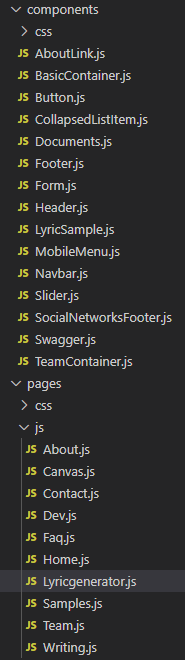
\includegraphics[width=5cm]{./imagenes/Desarrollo/AplicacionWeb/Paginas.png}
	\centering 
	\caption{Páginas trabajadas}
\end{figure}
La página más importe al momento de desarrollar la aplicación es la página principal, debido a que es esta la primera que va a ver el usuario al entrar y con la que más va a interactuar, en esta, aparece un mensaje con un botón el cual invita al usuario a generar su propia letra musical.
\begin{figure}[H]
	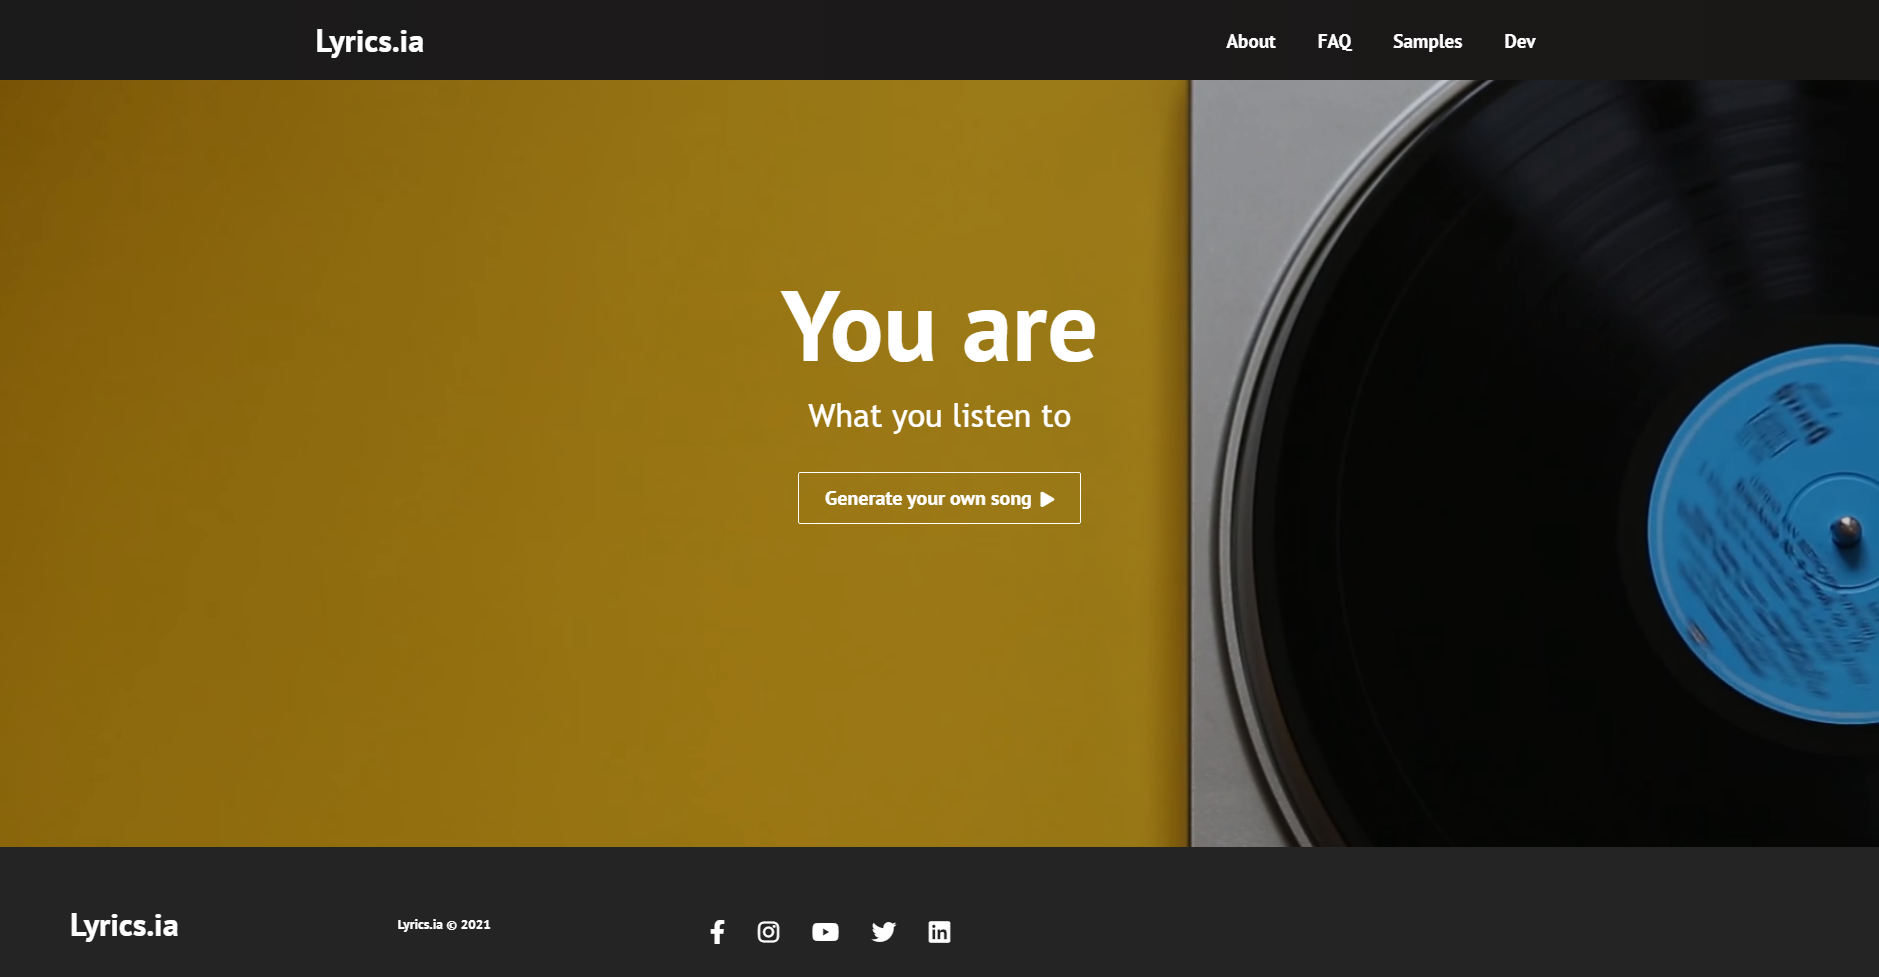
\includegraphics[width=13.5cm]{./imagenes/Desarrollo/AplicacionWeb/Pbienvenida.png}
	\centering 
	\caption{Página de bienvenida}
\end{figure}
Si el usuario le da clic al botón, como React usa estados para renderizar lo que ve el usuario, se muestra en pantalla el formulario donde se le pide al usuario que introduzca una palabra en el idioma inglés.
\begin{figure}[H]
	\includegraphics[width=13.5cm]{./imagenes/Desarrollo/AplicacionWeb/Pformulario.png}
	\centering 
	\caption{Formulario}
\end{figure}
Es en esta parte donde los datos proporcionados por el usuario son leídos y posteriormente enviados a nuestro back-end para ser procesados futuramente por el modelo. A continuación, se muestra el código de la función la cual realiza este proceso.
\begin{center}
	\lstinputlisting[language=JavaScript]{./imagenes/Desarrollo/AplicacionWeb/Sendword.js}
\end{center}
Esta función lo primero que se hace es recibir los datos (la palabra) que introdujo el usuario, esto se hace buscado el identificador del elemento de la página y obteniendo su valor, este, se enviará al back-end usando la función de fetch, lo que hace dicha función es buscar la url, que en este caso es donde se encuentra alojado nuestro back-end y busca el método post de este, como el método post de nuestro back-end recibe datos en formato json, los datos que introdujo el usuario deben ser enviados en este formato, usando JSON.stringfy y poniendole a la palabra un identificador que el back-end utilizará.\\\\
Después de que el usuario le dio clic al botón de generar canción se muestra una leyenda la cual le pide al usuario que espere unos segundos, que se está trabajando en su letra. Pasado un breve tiempo de espera, en pantalla se le mostrará la letra de la canción generada, esta presentación se realizara haciendo un efecto similar al de una máquina de escribir, así como 3 botones, el primero de ellos le permite descargar la letra generada en un archivo de texto, el segundo le permite al usuario generar una nueva canción utilizando los mismos parámetros con los que genero la letra actual y el ultimo lo regresa al estado anterior para introducir nuevos parámetros y con estos generar una nueva letra.
\begin{figure}[H]
	\includegraphics[width=13.5cm]{./imagenes/Desarrollo/AplicacionWeb/Pleyenda.png}
	\centering 
	\caption{Leyenda mostrada}
\end{figure}
\begin{figure}[H]
	\includegraphics[width=13.5cm]{./imagenes/Desarrollo/AplicacionWeb/Ptexto.png}
	\centering 
	\caption{Texto generado}
\end{figure}
Adentrándonos más en esta sección, la primera función que debemos revisar es la que permite hacer la conexión con el back-end para que la página pueda recibir el texto generado por el modelo.
\begin{center}
	\lstinputlisting[language=JavaScript]{./imagenes/Desarrollo/AplicacionWeb/ModelConection.js}
\end{center}
Lo que se hace en el código anterior es realizar una conexión asíncrona con el backend, esto para que mientras no se reciba una respuesta, el usuario en pantalla va a ver una leyenda que diga que se está trabajando en su texto, cuando en la conexión se reciba una respuesta la leyenda que ve el usuario cambiara, mostrando el texto recibido en la respuesta.
\begin{center}
	\lstinputlisting[language=JavaScript]{./imagenes/Desarrollo/AplicacionWeb/Download.js}
\end{center}
Con esta función se permite crear un archivo de texto el cual puede ser descargado en el equipo del usuario y el cual va a contener la letra de la canción que se generó en ese momento.
\begin{figure}[H]
	\includegraphics[width=10cm]{./imagenes/Desarrollo/AplicacionWeb/Archivo.png}
	\centering 
	\caption{Archivo de texto descargado}
\end{figure}	
Si el usuario utiliza el segundo botón, este, utilizando la misma palabra previamente introducido por el usuario llama a la función que conecta con el back-end enviándole una nueva petición de generación de texto y se renderiza nuevamente la vista con la leyenda de que espere unos segundos. En caso de utilizar el tercer botón solo activa el estado que renderiza la parte donde el usuario introduce los datos.
\newpage
\section{Desplegando componentes}

\subsection{Despliegue del backend}
Después de tener elaborada la API y hacer pruebas localmente haciendo llamadas desde cualquier terminal, se procedió a subirla para que los usuarios y la página web puedan hacer uso de ella desde cualquier parte del mundo.

Se utilizó Docker como herramienta, para posibilitar el despliegue de aplicaciones dentro de ``contenedores''. Esto permite que en cualquier hardware con Docker se pueda abrir la aplicación sin necesidad de tener que instalar y poner en marcha complejos programas. Al tener la imagen de la aplicación, se subió a  ``https://hub.docker.com/'', un servicio de registro de repositorios desarrollado por Docker inc. para alojar y descargar imágenes de Docker.

\begin{figure}[H]
	\includegraphics[width=12cm]{./imagenes/Desarrollo/AplicacionWeb/Archivo.png}
	\centering 
	\caption{Dockerfile para crear la imagen de la API}
\end{figure}

Se procedió a configurar y habilitar el acceso a Amazon Web Services para alojar la imagen de Docker y que pueda correr en un servidor de Amazon para que este disponible en la web, para ello se aseguró que el usuario creado fuera administrador y tuviera accesos para la creación de una instancia de EC2, un bucket de S3 y acceso a Amazon ElasticBeanstalk.

\begin{figure}[H]
	\includegraphics[width=12cm]{./imagenes/Desarrollo/AplicacionWeb/Archivo.png}
	\centering 
	\caption{Creación de usuario IAM en Amazon Web Services}
\end{figure}

Una vez creado el usuario, se hizo una instancia de EC2 y un bucket de S3 con Amazon ElasticBeanstalk, esta herramienta facilita la creación de API\'s con imágenes de docker y cuenta con muchas ventajas, entre ellas, versionamiento, la facilidad de ver la condición de la aplicación en tiempo real con registros de cada petición que se hace, junto con estadísticas útiles para ver el números de peticiones y manipular cualquier configuración necesaria para que la API pueda soportar cualquier


\subsection{Despliegue de la página web}

Para el despliegue de la pagina web nos apoyamos de la plataforma Vercel, la cual permite que los desarrolladores puedan desplegar sus paginas de manera rápida, así como poder actualizarla y escalarla de manera sencilla, además permite hacer despliegues de proyectos que se encuentran dentro de una cuenta de Github\\\\
Lo primero que debemos hacer para poder trabajar con la línea de comandos de Vercel es instalarlo, para ello debemos recurrir a nuestra terminal e instarlo usando el comando npm i -g vercel o yarn global add vercel.
\begin{figure}[H]
	\includegraphics[width=12cm]{./imagenes/Desarrollo/Despliegue/Instalacion.png}
	\centering 
	\caption{Instalando CLI de Vercel}
\end{figure}
Una vez instalado, debemos abrir la carpeta de nuestro proyecto a desplegar, y en una terminal dentro de esa carpeta solo es necesario escribir vercel para abrir el CLI de Vercel el cual nos preguntara si el proyecto contenido dentro de la carpeta es el que se va a configurar y desplegar, a lo cual damos una respuesta afirmativa, posteriormente nos pide quien lo va a desplegar, para ello usamos una cuenta creada en esta plataforma o vinculamos la de Github para acceder, se nos pregunta el nombre del proyecto y el inicio de los archivos del proyecto a desplegar.
\begin{figure}[H]
	\includegraphics[width=12cm]{./imagenes/Desarrollo/Despliegue/Acciones.png}
	\centering 
	\caption{Indicando acciones para el despliegue}
\end{figure}
Después de dar las indicaciones anteriores el CLI de vercel detecta automáticamente el tipo de proyecto trabajado, en este caso una aplicación web usando React, para por último preguntar si se quiere cambiar la configuración del trabajo encontrado, en este caso decimos que no, ya que es correcto el tipo de aplicación encontrada con el trabajado.
\begin{figure}[H]
	\includegraphics[width=12cm]{./imagenes/Desarrollo/Despliegue/Deteccion.png}
	\centering 
	\caption{Detección del tipo de proyecto a desplegar}
\end{figure}
Vercel comienza a desplegar la aplicación web y nos da un enlace en el cual podemos ver como se encuentra el despliegue, si se presentara algún problema, en la terminal nos indicara cual es.
\begin{figure}[H]
	\includegraphics[width=12cm]{./imagenes/Desarrollo/Despliegue/Desplegando.png}
	\centering 
	\caption{Desplegando el proyecto}
\end{figure}
Una vez completado el despliegue, se nos genera un enlace con el cual se puede acceder a la aplicación web ya desplegada desde cualquier dispositivo.
\begin{figure}[H]
	\includegraphics[width=12cm]{./imagenes/Desarrollo/Despliegue/Desplegada.png}
	\centering 
	\caption{Aplicación web desplegada}
\end{figure}
\begin{figure}[H]
	\includegraphics[width=12cm]{./imagenes/Desarrollo/Despliegue/Paginaweb.png}
	\centering 
	\caption{Accediendo a la aplicación web desplegada}
\end{figure}
En nuestro caso, previamente se había adquirido un dominio, para realizar el cambio del enlace proporcionado por Vercel al enlace del dominio previamente adquirido, en nuestro proyecto, en la parte de configuración, en la de domino, se agrega el enlace y así es posible acceder a esta pagina web desde ese dominio adquirido, este es  \textbf{www.neuralyrics.com}

\section{Pruebas}

En esta sección se observan capturas de pantalla de nuestra aplicación web, en ejecución, es decir, generando textos, permitiendo al usuario descargarlos, generar nuevos textos usando la misma palabra previamente introducida o con una nueva, así como dejándolo acceder a las distintas pestañas de la pagina web.

\subsection{Acceso a la aplicación web}

Lo primero que se debe hacer, es ingresar al sitio web \textbf{www.neuralyrics.com} y una vez este termine de desplegarse, se podrá empezar a interactuar.\\\\
\begin{figure}[H]
	\includegraphics[width=13cm]{./imagenes/Pruebas/pprincipal.png}
	\centering \caption{Pantalla principal al terminar la carga.}
\end{figure}
Al entrar, se muestra la siguiente pantalla donde se muestran dos leyendas breves y un botón invitando a empezar el funcionamiento principal de la aplicación web.
\begin{figure}[H]
	\includegraphics[width=13cm]{./imagenes/Pruebas/pprincipal.png}
	\centering \caption{Página de inicio de la aplicación web.}
\end{figure}

\subsection{Inicio de la generación de letras de canciones}

Si se da clic al botón mencionado anteriormente, se va a iniciar un efecto de desvanecimiento del texto de toda la pantalla para iniciar otro efecto para que aparezcan nuevas instrucciones en esta misma pantalla, todo esto sin necesidad de otra interacción, esto con el objetivo de que las distracciones se eliminen completamente y se pueda concentrar en el funcionamiento de la aplicación.
\begin{figure}[H] 
	\includegraphics[width=13.5cm]{./imagenes/Pruebas/pform.png}
	\centering \caption{Segunda pantalla al dar clic al botón principal.}
\end{figure}

\subsection{Segunda pantalla para generar letras de canciones}

La siguiente pantalla después del desvanecimiento, muestra instrucciones para ingresar una palabra en idioma inglés dentro de un campo vacío, así como un botón para empezar a generar la letra musical.
\begin{figure}[H] 
	\includegraphics[width=13.5cm]{./imagenes/Pruebas/pform.png}
	\centering \caption{Página del funcionamiento para generar una letra de canción.}
\end{figure}

Si el campo se deja vacío y se da clic al botón para generar una canción, se mostrará un mensaje obligando a rellenar el campo.

\begin{figure}[H] 
	\includegraphics[width=13.5cm]{./imagenes/Pruebas/Noword.png}
	\centering \caption{Mensaje mostrado si el campo se dejó vacío.}
\end{figure}

Para esta prueba se va a utilizar la palabra ``Madness'' como tema principal de la letra musical a generar

\begin{figure}[H] 
	\includegraphics[width=13.5cm]{./imagenes/Pruebas/Word.png}
	\centering \caption{Página de funcionamiento para generar una letra de canción usando la palabra ``Madness''.}
\end{figure}

\subsection{Resultado mostrando la letra de canción}
Después de dar clic al botón cumpliendo los requerimientos presentados en las instrucciones, se seguirá a una pantalla de carga en lo que se procesa la solicitud al sistema central de la aplicación, estos mensajes son para indicar al usuario que se esta trabajando en generar la letra musical y que espere un momento, evitando que este se frustre y recargue la pagina.

\begin{figure}[H] 
	\includegraphics[width=13.5cm]{./imagenes/Pruebas/pgenerating.png}
	\centering \caption{Pantalla de carga.}
\end{figure}

Una vez procesada la solicitud, se empezará a generar la canción con un efecto de typewriter y separando los versos y coros de la letra generada como resultado final, ademas de  tres botones diferentes, estos, mientras se esta generando la letra, se encontraran bloqueados.

\begin{figure}[H] 
	\includegraphics[width=13.5cm]{./imagenes/Pruebas/Generated.png}
	\centering \caption{Página con la letra generada.}
\end{figure}

Los botones que se pueden encontrar debajo de la letra generada son:

\begin{itemize}
	\item Download: Permite descargar la canción en formato txt.
	
	\begin{figure}[H] 
		\includegraphics[width=13.5cm]{./imagenes/Pruebas/Download.png}
		\centering \caption{Botón de descarga en funcionamiento.}
	\end{figure}

	\begin{figure}[H] 
		\includegraphics[width=13.5cm]{./imagenes/Pruebas/Textodescargado.png}
		\centering \caption{Documento con letra generada.}
	\end{figure}
	\newpage
	\item Regenerate Lyrics: Da la posibilidad de generar otra letra de canción con la misma palabra de la primera solicitud.
	
	\begin{figure}[H] 
		\includegraphics[width=13.5cm]{./imagenes/Pruebas/BotRegen.png}
		\centering \caption{Botón para generar lyric de nuevo.}
	\end{figure}
		
	\item Start Again: Lleva a la pantalla anterior para volver a rellenar el campo con la palabra deseada.
	
	\begin{figure}[H] 
		\includegraphics[width=13.5cm]{./imagenes/Pruebas/BotStart.png}
		\centering \caption{Botón para reiniciar el proceso.}
	\end{figure}	
	
\end{itemize}

Se hizo clic al botón Regenerate Lyrics para probar volver a generar otra letra de canción utilizando la misma palabra previamente introducida.

\begin{figure}[H] 
	\includegraphics[width=13.5cm]{./imagenes/Pruebas/Regenerate.png}
	\centering \caption{Letra de canción nuevamente generada usando la palabra ``Madness''.}
\end{figure}

De igual forma se hizo clic al botón Start Again para generar una nueva letra a partir de la la palabra ``Direction''.

\begin{figure}[H] 
	\includegraphics[width=13.5cm]{./imagenes/Pruebas/StartAgain.png}
	\centering \caption{Página con la letra generada a partir de una nueva palabra.}
\end{figure}

\subsection{Pantalla Developers}
Es una pantalla que muestra la documentación apropiada de la API generada a desarrolladores, en caso de que se requiera implementar llamadas al microservicio creado para poder generar lyrics, el usuario podrá acceder a esta pantalla y revisar los endpoints funcionales con una interfaz amigable para los desarrolladores.

\begin{figure}[H] 
	\includegraphics[width=13.5cm]{./imagenes/Pruebas/pdev.png}
	\centering \caption{Pantalla de developers mostrando los endpoints a los que se pueden acceder para llamar al microservicio.}
\end{figure}

\subsection{Pantalla Contact}
Permite tener contacto directo con los desarrolladores del micro-servicio y la página accediendo a esta pantalla, si se rellena el formulario con los datos de cada campo y dando clic al botón de “Enviar", se establecerá comunicación por medio de correo electrónico a la dirección ttlyrics.escom@gmail.com, el cual será revisado y contestado personalmente por algún integrante del equipo desarrollador.

\begin{figure}[H] 
	\includegraphics[width=13.5cm]{./imagenes/Pruebas/pcontact.png}
	\centering \caption{Pantalla de contacto.}
\end{figure}

\begin{figure}[H] 
	\includegraphics[width=13.5cm]{./imagenes/Pruebas/Correo.png}
	\centering \caption{Correo recibido.}
\end{figure}


\newpage

\section{Configuración de SSL y DNS}

Para permitir que nuestra pagina web pueda accederse desde otros dispositivos es necesario hacer la configuración correcta de DNS y darle un certificado de seguridad. Debido a que nuestra pagina web fue desplegada en la plataforma de Vercel, para que esta pueda direccionarse de manera correcta con nuestro dominio se requiere la configuración de un DNS especifico que nos pide Vercel.
\begin{figure}[H] 
	\includegraphics[width=10cm]{./imagenes/DnsSSL/Dns1.png}
	\centering \caption{Dirección IP requerida para la configuración del DNS.}
\end{figure}
\begin{figure}[H] 
	\includegraphics[width=10cm]{./imagenes/DnsSSL/Dns2.png}
	\centering \caption{Nombre requerido para la configuración del DNS.}
\end{figure}

Estas reglas de DNS deben agregarse en la plataforma de Cloudflare de la siguiente manera …..


En cuanto a la parte de seguridad de nuestra pagina web, como requiere que el usuario introduzca una palabra y esta posteriormente procesarla y mandarla a nuestro back-end, para ello se requirió configurar un certificado SSL para de esta manera tener una seguridad en el manejo de la información entre el servido del front-end y el back-end.\\\\
Para esta configuración nos apoyamos en Amazon Elastic Beans la cual nos permite darle el certificado que requiere el servidor del back-end siguiendo los siguientes pasos……


\chapter{\textcolor{azulescom}{Conclusiones}}

%%%%%%%%%%%%%%%%%%%%%%%%%%%%%%%%%%%%%%%%%%%%%%%%%%%%%%%%%
%                                                                                                                                                                                                 %
%                                                                                                                                                                                                 %
%                                                                Conclusiones del trabajo                                                                                  %
%                                                                                                                                                                                                 %
%                                                                                                                                                                                                 %
%%%%%%%%%%%%%%%%%%%%%%%%%%%%%%%%%%%%%%%%%%%%%%%%%%%%%%%%%

\newpage

\chapter{\textcolor{azulescom}{Trabajo a futuro}}

Después del lanzamiento inicial del proyecto, comenzamos a colaborar con algunos músicos para grabar las primeras canciones escritas por NeuraLyrics, que nos mostró la importancia de dar la
suficientes capacidades de personalización del usuario en lugar de simplemente
salida de letras completas. Con esto en mente, podría implementarse como trabajo a futuro:
\begin{enumerate} 
\item Mejorar la implementación de la generación del modelo para generar letras de canciones con más variedad.

\item Pida al algoritmo dar sugerencias para la siguiente línea y elegir la mejor sugerencia manualmente.

\item Dejar al usuario escribir algunas de las líneas manualmente, Un usuario puede, por ejemplo, escribir la primera línea por ellos mismos y dejar al algoritmo generar las líneas restantes. Un interesante modo de uso que notamos en algunos usuarios, es que prefieren escribir dos líneas manualmente y generar todas las demás con el modelo.

\item Poder generar textos con rimas, estas rimas se generarán a partir de la ultima palabra del primer verso de la letra de la canción generada, además se le pedirá al usuario que indique que tanto desea que rime una letra.\\\\
Las rimas generadas serás a partir de que estas se escriban de una manera similar a la palabra o que las estas suenen similares.\\\\
Se utilizaría la siguiente composición al momento de generar los textos
\begin{figure}[H]
	\includegraphics[width=12cm]{./imagenes/TrabajoFuturo/bert_output_model_rhyme.jpg}
	\centering 
	\caption{Estructura primer verso}
\end{figure}
\begin{figure}[H]
	\includegraphics[width=12cm]{./imagenes/TrabajoFuturo/Generacion_letras_rima.png}
	\centering 
	\caption{Estructura de la letra de la canción con rimas}
\end{figure}

\item Se puede utilizar la base de datos original o buscar otra con otros géneros musicales y realizar un procedimiento similar al que se siguió para conseguir el conjunto de datos de las letras de canciones del género pop.\\\\
Una vez obtenidos los conjuntos de datos separados de los géneros que queremos trabajar, hacer modelos usando redes neuronales y añadirlos a nuestro backend.\\\\
Para que de esta forma si el usuario en la pagina principal decide crear una canción, se le muestre que puede seleccionar un genero musical que previamente se ha trabajado.
\end{enumerate}

% Rename Appendice to Anexos
\renewcommand*\appendixpagename{{\textcolor{azulescom}{Anexos}}}
\renewcommand*\appendixtocname{{\textcolor{azulescom}{Anexos}}}
\pagebreak
\appendixpageon
	\begin{appendices}
	% Cadenas de Markov
	\centering
	\section{Cadenas de Markov}
	\includepdf[pages=-]{./anexos/CadenasdeMarkov.pdf}\label{prueba2}
	%%Glosario
	\newpage
		\section{Pruebas utilizando long short term memories}
		\includepdf[pages=-]{./anexos/LSTM.pdf}\label{pruebaslstm}
	\newpage
	\renewcommand*\glossaryname{{\textcolor{azulescom}{Glosario}}}
	\printglossary
	%%Acrónimos
	\newpage
	\renewcommand*\glossaryname{{\textcolor{azulescom}{Acrónimos}}}
	\printglossary[title={\textcolor{azulescom}{Acrónimos.}}, type=\acronymtype]
\end{appendices}
%%%%%%%%%%%%%%%%%%%%%%%%%%%%%%%%%%%%%%%%%%%%%%%%%%%%%%%%%
%                                                       																																		  %
%                                                      																																	  		  %
%              																	 Bibliografía  																				  			%
%                                                      																																			  %
%                                                      																																			  %
%%%%%%%%%%%%%%%%%%%%%%%%%%%%%%%%%%%%%%%%%%%%%%%%%%%%%%%%%
\begin{thebibliography}{20}
	%Glosario
	\bibitem{refRAE} 	
	Real Academia Española (2020, noviembre), Diccionario de la lengua española, [En línea]. Disponible: https://dle.rae.es [Último acceso: 10 de diciembre del 2020].
	
	\bibitem{refOxfordLex} 
	Oxford Lexico (2020, noviembre), Definitions, Meanings, Synonyms, and Grammar by Oxford, [En línea]. Disponible: https://www.lexico.com [Último acceso: 2 de diciembre del 2020].
	
	\bibitem{refMaquinasFinitas} 	
	J. A. Gutiérrez Orozco, Escuela Superior de Cómputo (2008, septiembre 15), Máquinas de Estados Finitos, [En línea]. Disponible: http://delta.cs.cinvestav.mx/~mcintosh/cellularautomata/Summer\_Research\_files/maquinasef.pdf [Último acceso: 15 de diciembre del 2020].
	
	\bibitem{refSistema} 
	O. Jaramillo, Universidad Nacional Autonoma de México (2007, mayo 03), El concepto de Sistema, [En línea]. Disponible: https://www.ier.unam.mx/~ojs/pub/Termodinamica/node9.html [Último acceso: 2 de diciembre del 2020].
	% Introducción
	\bibitem{Bourreau_and_Gensollen} 	
	Chaney, D. (2012). The Music Industry in the Digital Age: Consumer Participation in Value Creation. International Journal of Arts Management, (1), pp. 15.
	
	\bibitem{Generating_Text_with_RNN} 
	Sutskever, I., Martens, J., Hinton, G. E. (2011, January). Generating text with recurrent neural networks. In ICML.
	
	\bibitem{CNN_for_Sentence_Classification} 
	Kim, Y. (2014). Convolutional neural networks for sentence classification. arXiv preprint arXiv:1408.5882.
	
	\bibitem{Automatic_Generation_of_Melodic_Accompaniments_for_Lyrics} 
	Monteith, K., Martinez, T. R., \& Ventura, D. (2012, May). Automatic Generation of Melodic Accompaniments for Lyrics. In ICCC, pp. 87-94.
	
	\bibitem{Conditional_Rap_Lyrics_Generation} 
	Nikolov, N. I., Malmi, E., Northcutt, C. G., Parisi, L. (2020). Conditional Rap Lyrics Generation with Denoising Autoencoders. arXiv preprint arXiv:2004.03965.
	
	% Justificación
	\bibitem{What_about_the_music} 
	Baker, F. A. (2015). What about the music? Music therapists’ perspectives on the role of music in the therapeutic songwriting process. Psychology of Music, 43(1), pp. 122-139.
	
	\bibitem{genero_musical_en_la_musica_popular} 
	Guerrero, J. (2012). El género musical en la música popular: algunos problemas para su caracterización. Trans. Revista transcultural de música, (16), pp. 1-22.
	
	\bibitem{Bert} 
	Wang, A., \& Cho, K. (2019). Bert has a mouth, and it must speak: Bert as a markov random field language model. arXiv preprint arXiv:1902.04094.
	
	\bibitem{spaCy} 
	Honnibal, M.,\& Montani, I. (2017). spaCy 2: Natural language understanding with Bloom embeddings, convolutional neural networks and incremental parsing.
	% Marco Teórico IA
	\bibitem{Inteligencia_Artificial}
	V. Advani (2021, febrero 11), What is Artificial Intelligence? How does AI work, Types and Future of it?, [En línea]. Disponible:https://www.mygreatlearning.com/blog/what-is-artificial-intelligence/ [Último acceso: 6 de abril del 2021].
	
	\bibitem{refInteligencia_Artificial2}
	IBM Corporation (2021, marzo 31), Artificial Intelligence (AI), [En línea]. Disponible: https://www.ibm.com/cloud/learn/what-is-artificial-intelligence [Último acceso: 6 de abril del 2021].
	
	% Marco Teórico Neural Networks
	\bibitem{refQueSonRedesNeu} 	
	L. Hardesty (2017, abril), Explained: Neural networks, [En línea]. Disponible: https://news.mit.edu/2017/explained-neural-networks-deep-learning-0414 [Último acceso: 15 de noviembre del 2020].	
	
	% Redes Neuronales
	\bibitem{refNeuronaNat}
	amBientech (2019, julio 30), ¿Qué es la neurona?, [En línea]. Disponible: https://ambientech.org/la-neurona [Último acceso: 6 de abril del 2021].
	\bibitem{refNeuronaNat2}
	National Cancer Institute (2021), Neurons \& Glial Cells, [En línea]. Disponible: https://training.seer.cancer.gov/brain/tumors/anatomy/neurons.html [Último acceso: 30 de abril del 2021].	
	\bibitem{refNeuronaArt}
	C. Gershenson (2012, octubre), Artificial Neural Networks for Beginners, [En línea]. Disponible: https://www.uv.mx/mia/files/2012/10/Artificial-Neural-Networks-for-Beginners.pdf [Último acceso: 6 de abril del 2021].
	\bibitem{refAprendizajeRedes} 
	Rubik's Code (2018, febrero), How do Artificial Neural Networks learn?, [En línea]. Disponible: https://rubikscode.net/2018/01/15/how-artificial-neural-networks-learn/ [Último acceso: 7 de abril del 2021].	
	\bibitem{refTiposRedesNeu1} 	
	S. Leijnen, F. van Veen (2020, mayo), The Neural Network Zoo, [En línea]. Disponible: https://www.researchgate.net/publication/341373030\_The\_Neural\_Net\\work\_Zoo [Último acceso: 20 de noviembre del 2020].
	\bibitem{refTiposRedesNeu4} 
	IBM Cloud Education (2020, septiembre 14), What are Recurrent Neural Networks?, [En línea]. Disponible: https://www.ibm.com/cloud/learn/recurrent-neural-networks [Último acceso: 26 de marzo del 2021].
	
	%PLN
	\bibitem{refProcesamientoLN}
	ref IBM Cloud Education (2020, julio 2), Natural Language Processing [En línea]. Disponible: https://www.ibm.com/cloud/learn/natural-language-processing [Ultimo acceso: 20 de abril del 2021].
	
	%Transformer
	\bibitem{refQueesuntransformer} 
	ref A. Vaca (2020, mayo), Transformers en Procesamiento del Lenguaje Natural, [En línea]. Disponible: https://www.iic.uam.es/innovacion/transformers-en-procesamiento-del-lenguaje-natural/ [Ultimo acceso: 15 de abril del 2021].
	\bibitem{refArqTransformer} 
	ref A. Vaswani, N. Shazeer, N. Parmar, J. Uszkoreit, L. Jones, A. Gomez, L. Kaiser \& I. Polosukhin (2017, diciembre), Attention Is All You Need, [En línea]. Disponible: https://arxiv.org/pdf/1706.03762.pdf [Ultimo acceso: 15 de abril del 2021].
	
	% Bert
	\bibitem{refQueesBert} 
	ref J. Devlin, M. Chang, K. Lee, K. Toutanova (2019, mayo), BERT: Pre-training of Deep Bidirectional Transformers for
	Language Understanding, [En línea]. Disponible: https://arxiv.org/pdf/1810.04805.pdf [Ultimo acceso: 11 de abril del 2021].
	\bibitem{refComofuncionaBert} 
	ref R. Horev (2018, noviembre), BERT Explained: State of the art language model for NLP, [En línea]. Disponible: https://towardsdatascience.com/bert-explained-state-of-the-art-language-model-for-nlp-f8b21a9b6270 [Ultimo acceso: 11 de abril del 2021].
	\bibitem{refBertactualidad} 
	ref B. Lutkevich (2020, enero), BERT language model, [En línea]. Disponible: https://searchenterpriseai.techtarget.com/definition/BERT-language-model [Ultimo acceso: 12 de abril del 2021].
	
	%GPT-2
	\bibitem{refQueesgpt} 
	ref A. Radford, J. Wu, D. Amodei, D. Amodei, J. Clark, M. Brundage \& I. Sutskever (2020, enero), Better Language Models and Their Implications, [En línea]. Disponible: https://openai.com/blog/better-language-models/ [Ultimo acceso: 14 de abril del 2021].
	\bibitem{refbpe} 
	ref M. Edward (2019, febrero), Too powerful NLP model (GPT-2), [En línea]. Disponible: https://towardsdatascience.com/too-powerful-nlp-model-generative-pre-training-2-4cc6afb6655 [Ultimo acceso: 14 de abril del 2021].
	\bibitem{refarquitecturagpt} 
	ref A. Radford, K. Narasimhan, T. Salimans \& I. Sutskever (2018), Improving Language Understanding by Generative Pre-Training, [En línea]. Disponible: https://s3-us-west-2.amazonaws.com/openai-assets/research-covers/language-unsupervised/language\_understanding\_paper.pdf [Ultimo acceso: 14 de abril del 2021].
	\bibitem{refarquitecturagpt2} 
	ref J. Montantes(2019, mayo), Examining the Transformer Architecture, [En línea]. Disponible: https://towardsdatascience.com/examining-the-transformer-architecture-part-1-the-openai-gpt-2-controversy-feceda4363bb [Ultimo acceso: 14 de abril del 2021].
	\bibitem{refarquitecturagpt3}
	ref J. Vig(2019, marzo), GPT-2: Understanding Language Generation through Visualization, [En línea]. Disponible: https://towardsdatascience.com/openai-gpt-2-understanding-language-generation-through-visualization-8252f683b2f8 [Ultimo acceso: 14 de abril del 2021].
	
	%Bases de Datos
	\bibitem{refQueEsBD} 	
	Oracle México (2020, noviembre), ¿Qué es una base de datos?, [En línea]. Disponible: https://www.oracle.com/mx/database/what-is-database/ [Último acceso: 20 de noviembre del 2020].
	
	% Canción
	\bibitem{refEstructuraCancion1} 
	Escribir Canciones (2008), Estructura y elementos de una canción, [En línea]. Disponible: https://dle.rae.es [Último acceso: 2 de diciembre del 2020].
	\bibitem{refEstructuraCancion2} 
	Swing this Music (2008), ¿QUÉ SECCIONES PUEDE TENER UNA CANCIÓN?española, [En línea]. Disponible: https://sites.google.com/site/swingthismusiccast/interpretacio/estruct\\ura-cancion/secciones-de-una-cancion [Último acceso: 2 de diciembre del 2020].
	
	% Markov
	\bibitem{refMarkov} 
	J. R. Norris (1997), Markov Chains, [En línea]. Disponible: https://cape.fcfm.buap.mx/jdzf/cursos/procesos/libros/norris.pdf [Último acceso: 15 de diciembre del 2020].
	
	\bibitem{refNginx} 
	NGINx (2016, mayo 17), What is NGINX?, [En línea]. Disponible: https://www.nginx.com/resources/glossary/nginx/ [Último acceso: 27 de mayo del 2021].
	
	%Herramientas a usar Software
	
	\bibitem{refHtml}
	Mozilla.org (2021, febrero 19), HTML basics, [En línea]. Disponible: https://developer.mozilla.org/en-US/docs/Learn/Getting\_started\_with\_the\_web/HTML\_basics [Último acceso: 15 de mayo del 2021].
	\bibitem{refHtml2}
	Mozilla.org (2021, mayo 14), HTML5, [En línea]. Disponible: https://developer.mozilla.org/es/docs/Web/Guide/HTML/HTML5 [Último acceso: 15 de mayo del 2021].
	\bibitem{refcss}
	W3C (2016), HTML \& CSS, [En línea]. Disponible: [Último acceso: 15 de mayo del 2021].
	\bibitem{refjs}
	Mozilla.org (2021, abril 27), What is JavaScript?, [En línea]. Disponible: https://developer.mozilla.org/en-US/docs/Learn/JavaScript/First\_steps/What\_is\_JavaScript [Último acceso: 15 de mayo del 2021].
	\bibitem{refopenssl}
	OpenSSL (2018), OpenSSL, [En línea]. Disponible: https://www.openssl.org [Último acceso: 15 de mayo del 2021].
	
	% Apache
	\bibitem{Apache} 		
	Documentation Group. (n.d.). Welcome! - The Apache HTTP Server Project. Apache. Retrieved April 6, 2021, from https://httpd.apache.org/
	\bibitem{what_is_apache} 	
	G., D. (2021, March 9). What is Apache? An In-Depth Overview of Apache Web Server. Hostinger Tutorials. https://www.hostinger.com/tutorials/what-is-apache
	
	% Servidor Web
	\bibitem{What_is_a_web_server}		
	What is a web server? - Learn web development | MDN. (2021, January 27). MDN Web Docs. https://developer.mozilla.org/en-US/docs/Learn/Common\_questions/What\_is\_a\_web\_server
	
	% Certificado SSL
	\bibitem{what_is_SSL} 
	What is SSL? (2017, May 15). SSLSHOPPER. https://www.sslshopper.com/what-is-ssl.html
	\bibitem{ssl_certificates} 
	Verisign. (2015, August 30). ¿Qué es un certificado SSL? – Verisign. Verisign NameStudio. https://www.verisign.com/es\_LA/website-presence/online/ssl-certificates/index.xhtml
	
	% Plataforma en la nube de ML 
	\bibitem{data_science_in_the_cloud} 
	Bavati, I. (2020, September 22). Data Science in the Cloud - Towards Data Science. Medium. https://towardsdatascience.com/data-science-in-the-cloud-239b795a5792 (September 2020)
	\bibitem{comparing-google-cloud-platform-aws-and-azure} 
	G. (2021, March 5). Comparing Google Cloud Platform, AWS and Azure - Georgian Impact Blog. Medium. https://medium.com/georgian-impact-blog/comparing-google-cloud-platform-aws-and-azure-d4a52a3adbd2
	\bibitem{what_is_jupyter} 
	I., A. (2015, October 2). Jupyter/IPython Notebook Quick Start Guide. Jupyter Notebook Beginner Guide. https://jupyter-notebook-beginner-guide.readthedocs.io/en/latest/what\_is\_jupyter.html
	\bibitem{google_cloud_vs_aws} 
	Jones, E. (2021, March 25). Google Cloud vs AWS in 2021 (Comparing the Giants). Kinsta. https://kinsta.com/blog/google-cloud-vs-aws/
	
	% Aspectos Legales	
	\bibitem{refCopyright} 	
	Copyright.gov (2021), Copyright in General, [En línea]. Disponible: https://www.copyright.gov/help/faq/faq-general.html\#what [Último acceso: 04 de mayo del 2021].
	
	\bibitem{refOriginalidadWipo} 	
	World Intellectual Property Organization (2007), THE ARTS AND COPYRIGHT, [En línea]. Disponible: https://www.wipo.int/edocs/pubdocs/en/copyright/935/wipo\_pub\_935\\.pdf [Último acceso: 04 de mayo del 2021].
	
	\bibitem{refOriginalidadLFDA} 
	CÁMARA DE DIPUTADOS DEL H. CONGRESO DE LA UNIÓN (2014, julio 14), LEY FEDERAL DEL DERECHO DE AUTOR, [En línea]. Disponible: https://www.ucol.mx/content/cms/13/file/federal/\\LEY\_FED\_DEL\_DERECHO\_DEL\_AUTOR.pdf [Último acceso: 05 de mayo del 2021].
	
	% Iteración 2
	\bibitem{data_cleaning}
	Aaron Tay (2021, Abril 23), Data Cleaning Techniques [En línea]. Disponible: https://www.digitalvidya.com/blog/data-cleaning-techniques/ [Último acceso: 30 Mayo 2021]
	%-------Referencias Herramientas a usar---------%
	\bibitem{refQuesPython} 
	Python (2021), What is Python? Executive Summary, [En línea]. Disponible: https://www.python.org/doc/essays/blurb/ [Último acceso: 24 de abril del 2021].
	
	%---------------------------Referencias Originales ↓----------------------------%
	
	
	\bibitem{refMongoDB}
	MongoDB. (2019), ¿Qué es MongoDB?, [En línea]. Disponible: https://www.mongodb.com/es. [Último acceso: 26 Marzo 2021].
	
	\bibitem{refNodeOpenSSL}
	Noteworthy Programming Masterpiece (2019), openssl-nodejs [En línea]. Disponible: https://www.npmjs.com/package/openssl-nodejs [Último acceso: 26 Marzo 2021]
	
	\bibitem{refTomcat}
	The Apache Software Foundation (2019), Apache Tomcat [En línea]. Disponible: http://tomcat.apache.org/index.html [Último acceso: 26 Marzo 2021]
	
	\bibitem{refDatamuseLicense}
	OneLook Dictionary Search (2016), Privacy Policy [En línea]. Disponible: https://www.onelook.com/about.shtml [Último acceso: 19 Mayo 2021]
	
	\bibitem{refMongoDBLicense}
	MongoDB Inc (2018), MongoDB Licensing [En línea]. Disponible: https://www.mongodb.com/community/licensing [Último acceso: 19 Mayo 2021]
	
	\bibitem{refBERTLicense}
	Google Research: BERT (2018), LICENSE [En línea]. Disponible: https://github.com/google-research/bert/blob/master/LICENSE [Último acceso: 19 Mayo 2021]
	
	\bibitem{refApacheLicense}
	Apache (2004), The Apache License, Version 2.0 [En línea]. Disponible: https://httpd.apache.org/docs/current/license.html [Último acceso: 19 Mayo 2021]
	
	\bibitem{refReactLicense}
	Facebook: React (2018), LICENSE [En línea]. Disponible: https://github.com/facebook/react/blob/master/LICENSE [Último acceso: 19 Mayo 2021]
	
	\bibitem{refPythonLicense}	
	Python (2001), History and License [En línea]. Disponible: https://docs.python.org/3/license.html [Último acceso: 19 Mayo 2021]
	
	\bibitem{refAmazonLicense}
	Elastic (2021), Elastic License 2.0 [En línea]. Disponible: https://www.elastic.co/es/licensing/elastic-license [Último acceso: 19 Mayo 2021]
	
	\bibitem{refGoogleCloudPlatform}
	Google Cloud Platform (2021), Descripción general de Google Cloud [En línea]. Disponible: https://cloud.google.com/docs/overview [Último acceso: 25 Mayo 2021]
	
	\bibitem{refAmazonWebServices}
	Amazon Web Services (2021), Informática en la nube con AWS [En línea]. Disponible: https://aws.amazon.com/es/what-is-aws/ [Último acceso: 25 Mayo 2021]
	
	\bibitem{refAzure}
	Azure (2021), Conozca Azure [En línea]. Disponible: https://azure.microsoft.com/es-mx/overview/ [Último acceso: 25 Mayo 2021]
	
	\bibitem{refMatrizEvaluacionRiesgos}
	ITM Platform (2010), Matriz de Evaluación de Riesgos [En línea]. Disponible: https://www.itmplatform.com/es/recursos/matriz-de-evaluacion-de-riesgos
	/\#RiskSetId=rh25q/6IQWFCFvYIwSUF6A== [Último acceso: 26 Mayo 2021]
	
	\bibitem{kaggle}
	Kaggle (2010), How to Use Kaggle [En línea]. Disponible: https://www.kaggle.com/docs/datasets [Último acceso: 25 Mayo 2021]
	
	\bibitem{kaggleDataset}
	Kaggle (2019, Noviembre 17), Song lyrics from 6 musical genres [En línea]. Disponible: https://www.kaggle.com/neisse/scrapped-lyrics-from-6-genres [Último acceso: 25 Mayo 2021]
		
	\bibitem{googleDatasets}
	Google (2018, Septiembre 5), Dataset Search [En línea]. Disponible: https://datasetsearch.research.google.com [Último acceso: 25 Mayo 2021]
	
	\bibitem{awsOpenData}
	Amazon, Open Data on AWS [En línea]. Disponible: https://aws.amazon.com/es/opendata/?wwps-cards.sort-by=item.additionalFields.sortDate\&wwps-cards.sort-order=desc [Último acceso: 25 Mayo 2021]
	
	\bibitem{music4all}
	Music4All (2020), A New Music Database and Its Applications [En línea]. Disponible: https://sites.google.com/view/contact4music4all [Último acceso: 25 Mayo 2021]
	
	\bibitem{vagalume}
	Vagalume (2002), Vagalume: Music e tudo [En línea]. Disponible: https://www.vagalume.com.br/ [Último acceso: 25 Mayo 2021]
	
	\bibitem{top_ten_lyric}
	TopTenAI (2020, Mayo 9), Top 10 Lyric Generator Review 2021 [En línea]. Disponible: https://topten.ai/lyric-generator-review/ [Último acceso: 30 Mayo 2021]
	
	\bibitem{adam}
	Kingma, D. P., Ba, J. (2014). Adam: A method for stochastic optimization. arXiv preprint arXiv:1412.6980.
	
	\bibitem{adam2}
	Sanjeevi, M. (2018, June 21). Chapter 10.1: DeepNLP — LSTM (Long Short Term Memory) Networks with Math. Medium. https://medium.com/deep-math-machine-learning-ai/chapter-10-1-deepnlp-lstm-long-short-term-memory-networks-with-math-21477f8e4235
	 
	\bibitem{HistoriaNPL}
	Foote, K. D. (2019, June 17). A Brief History of Natural Language Processing (NLP). DATAVERSITY. https://www.dataversity.net/a-brief-history-of-natural-language-processing-nlp/
	 
	\bibitem{amazon_ec2}
	Amazon (2021), Amazon EC2 [En línea]. Disponible: https://aws.amazon.com/es/ec2/?ec2-whats-new.sort-by=item.additionalFields.postDateTime\&ec2-whats-new.sort-order=desc [Último acceso: 1 Junio 2021]
	
	\bibitem{amazon_sagemaker}
	Amazon (2021), Amazon SageMaker [En línea]. Disponible: https://aws.amazon.com/es/sagemaker/ [Último acceso: 1 Junio 2021]
	
	\bibitem{amazon_s3}
	Amazon (2021), Amazon S3 [En línea]. Disponible: https://aws.amazon.com/es/s3/ [Último acceso: 1 Junio 2021]
	
	\bibitem{PruebaLSTM}
	Bansal, S. (2018, May 27). Language Modelling and Text Generation using LSTMs — Deep Learning for NLP. Medium. https://medium.com/@shivambansal36/language-modelling-text-generation-using-lstms-deep-learning-for-nlp-ed36b224b275
	
	\bibitem{tokenimagen}
	B. Lee (2019, Noviembre 17), How to 10x Response Rates on Surveys [En línea]. Disponible: https://bryankmlee3.medium.com/conducting-surveys-with-nlp-d38df4c29e39 [Último acceso: 5 Junio 2021]
	
\end{thebibliography}	
\end{document}



